% start the document
% NOTE: Previous version was main-frankenstein-2.tex

% NEW FIGURES/CALCULATIONS
% 1. modified version of Fig. 1 from the CMS paper of a spherical voronoi diagram, where you show the reference point, all of its symmetric images, and maybe just color the cell in which the reference point falls a different color to indicate that that region is the VFZ since it is closer to the reference point than to any of its symmetric images.
% 2. teaching figure for generating VFZ point set and then making the GB energy landscape
% 2. generate N octonions (both methods), calculate pairwise distances, NN distribution, etc.
% 3. get pairwise distances for GBs in each respective dataset
% 4. how to remake & edit tunnel plots
% 5. details of GPR method & options used

% specify the document layout and font size
%\documentclass[review,12pt]{elsarticle}
\documentclass[final,twocolumn,12pt]{elsarticle}
\usepackage[margin=1.5cm,includefoot]{geometry}
\usepackage{auto-paper}
\PassOptionsToPackage{refcheck}{auto-paper} %comment this out before submission
\usepackage{dcolumn}

\newcolumntype{d}[1]{D{.}{.}{#1}}

\zexternaldocument*{supp-frankenstein-2}
% Concatenate the different "values" .tex files
%RMSE values
% \newcommand{\baryrmse}{0.0242}
% \newcommand{\gprrmse}{0.0220}
% \newcommand{\idwrmse}{0.0345}
% \newcommand{\nnrmse}{0.0448}
% \newcommand{\avgrmse}{0.1302}
% %paper-data6
% \newcommand{\baryrmse}{0.0238}
% \newcommand{\gprrmse}{0.0218}
% \newcommand{\idwrmse}{0.0356}
% \newcommand{\nnrmse}{0.0445}
% \newcommand{\avgrmse}{0.1283}
%\newcommand{\gprrmsePercReduction}{83}
% paper-data9
\newcommand{\baryrmse}{0.0239}
\newcommand{\gprrmse}{0.0217}
\newcommand{\idwrmse}{0.0343}
\newcommand{\nnrmse}{0.0448}
\newcommand{\avgrmse}{0.1284}
\newcommand{\gprrmsePercReduction}{83.1}

%MAE values
% \newcommand{\barymae}{0.0145}
% \newcommand{\gprmae}{0.0145}
% \newcommand{\idwmae}{0.0223}
% \newcommand{\nnmae}{0.0307}
% \newcommand{\avgmae}{0.0965}
% %paper-data6
% \newcommand{\barymae}{0.0145}
% \newcommand{\gprmae}{0.0145}
% \newcommand{\idwmae}{0.0225}
% \newcommand{\nnmae}{0.0307}
% \newcommand{\avgmae}{0.0955}
%paper-data9
\newcommand{\barymae}{0.0145}
\newcommand{\gprmae}{0.0145}
\newcommand{\idwmae}{0.0223}
\newcommand{\nnmae}{0.0308}
\newcommand{\avgmae}{0.0959}

%\newcommand{\nnomega}{2.8709 \pm 0.69112}
\newcommand{\nnomega}{2.8702 \pm 0.69117}

\newcommand{\symtime}{76}

\newcommand{\nigprbrkrmse}{0.1471}

%Supplementary
\newcommand{\thr}{\SI{1.1}{\joule\per\square\meter}}
\newcommand{\sigthr}{\SI{1.1}{\joule\per\square\meter}}
\newcommand{\thrtwo}{\SI{1.2}{\joule\per\square\meter}}


%% main-frankenstein-2
\newcommand{\minsymdist}{$\sim$\SI{64.0}{\tobydeg}}
\newcommand{\percExplained}{$\sim$\SI{99.6}{\percent}}
\newcommand{\percFiveVsOne}{$\sim$\SI{70}{\percent}}
\newcommand{\dimOne}{$\sim$\SI{65}{\tobydeg}}

% figure info, etc. that can dynamically change (color of points, etc.)
\newcommand{\startpt}{red points}
\newcommand{\singlept}{magenta points}
\newcommand{\sympt}{dark blue points}
\newcommand{\singlesympt}{dark blue point}
\newcommand{\refpt}{white circle}
\newcommand{\vbordercolor}{black}
\newcommand{\vcellcolor}{light blue}
\newcommand{\inpt}{input}
\newcommand{\outpt}{prediction}
% \newcommand{\inptvar}{ninputpts}
% \newcommand{\distfn}{GBdist4}
\newcommand{\vfzorepo}{\gls{vfz} repository}
\newcommand{\mytitleone}{Five Degree-of-Freedom Property Interpolation of Arbitrary Grain Boundaries via \glsentrytitlecase{vfz}{long} Framework}
% \newcommand{\mytitletwo}{Properties of a \glsentrytitlecase{5dof}{long} \glsentrytitlecase{fz}{long} defined via \glsentrytitlecase{vfz}{long} Framework}
\newcommand{\mytitletwo}{$O_h$ \glsentrytitlecase{5dof}{long} \glsentrytitlecase{fz}{long} Properties via \glsentrytitlecase{vfz}{long} Framework}
\makeglossaries
\GlsXtrEnableEntryCounting{abbreviation}{3}
% \glssetcategoryattribute{abbreviation}{indexonlyfirst}{true}
\glssetcategoryattribute{abbreviation}{nohyper}{true}

% \setabbreviationstyle[abbreviation]{long-short}

% \glsenableentrycount
% \glssetcategoryattribute{abbreviation}{entrycount}{2}

\newabbreviation[longplural=five degrees of freedom]{5dof}{5DOF}{five degree-of-freedom}
\newabbreviation[longplural=three degrees of freedom]{3dof}{3DOF}{three degree-of-freedom}
\newabbreviation[longplural=degrees of freedom]{dof}{DOF}{degree of freedom}
\newabbreviation{ebsd}{EBSD}{electron backscatter diffraction}
\newabbreviation[longplural={grain boundaries}]{gb}{GB}{grain boundary}
\newabbreviation{fcc}{FCC}{face-centered cubic}
\newabbreviation{sem}{SEM}{scanning electron microscope}
\newabbreviation{fea}{FEA}{finite element analysis}
\newabbreviation{bcs}{BCs}{boundary conditions}
\newabbreviation[longplural={triple junctions}]{tj}{TJ}{triple junction}
\newabbreviation{gpr}{GPR}{Gaussian process regression}
\newabbreviation{gprm}{GPRM}{Gaussian process regression mixture}
\newabbreviation{ann}{ANN}{artificial neural network}
\newabbreviation{nn}{NN}{nearest neighbor}
\newabbreviation{rmse}{RMSE}{root mean square error}
\newabbreviation{mae}{MAE}{mean absolute error}
\newabbreviation{brk}{BRK}{Bulatov Reed Kumar}
\newabbreviation{gbed}{GBED}{grain boundary energy distribution}
\newabbreviation{gbcd}{GBCD}{grain boundary character distribution}
\newabbreviation{mfz}{MFZ}{misorientation fundamental zone}
\newabbreviation{bp}{BP}{boundary plane}
\newabbreviation{bpfz}{BPFZ}{boundary plane fundamental zone}
\newabbreviation{knn}{kNN}{k-nearest neighbor}
\newabbreviation{gbe}{GBE}{grain boundary energy}
\newabbreviation{gbo}{GBO}{grain boundary octonion}
\newabbreviation{nbo}{NBO}{no-boundary octonion}
\newabbreviation{oslerp}{oSLERP}{octonion Spherical Linear Interpolation}
\newabbreviation{loocv}{LOOCV}{leave-one-out cross validation}
\newabbreviation{kfcv}{kFCV}{k-fold cross validation}
\newabbreviation{seo}{SEO}{symmetrically equivalent octonion}
\newabbreviation{fex}{FEX}{file exchange}
\newabbreviation{idw}{IDW}{inverse-distance weighting}
\newabbreviation{fic}{FIC}{fully independent conditional}
\newabbreviation{svd}{SVD}{singular value decomposition}
\newabbreviation{gbc}{GBC}{grain boundary character}
\newabbreviation{fz}{FZ}{fundamental zone}
% \newabbreviation{pfz}{pFZ}{pseudo fundamental zone} % pfz replaced by vfz
% \newabbreviation{cmo}{CMO}{closed-mesh octonion} % cmo replaced by vfzo
\newabbreviation{vfz}{VFZ}{Voronoi fundamental zone}
\newabbreviation{vfzgbo}{VFZ-GBO}{Voronoi fundamental zone grain boundary octonion}
\newabbreviation{lobpcg}{LOBPCG}{locally optimal block preconditioned conjugate gradient}
\newabbreviation{lkr}{LKR}{Laplacian kernel regression}
\newabbreviation{ms}{MS}{molecular statics}
\newabbreviation{sst}{SST}{standard stereographic triangle}
\newabbreviation{ml}{ML}{machine learning}
\newabbreviation{doe}{DoE}{design of experiments}
\newabbreviation{ct}{CT}{coherent-twin}
% example abbreviations
% \newabbreviation{seo}{SEO}{symmetrically equivalent octonions}
%\newabbreviation[longplural={grain boundaries}]{gb}{GB}{grain boundary}

%example usage: \gls{gpr}
%example usage: \Gls{gpr} (capitalize first letter, only meaningful for first usage)
% \glspl{seo} --> symmetrically equivalent octonions OR SEOs
%^^^^^^^^^^^^^^^^^^^^^^^^^^^^^^^^^^^^^^^^^^^^^^^^^^^


\DeclareSIUnit \tobydeg {\!\degree\mbox{$\ \left[d_{\Omega}\right]$}}
\DeclareSIUnit \eucdeg {\!\degree\mbox{$\ \left[d_{\text{E}}\right]$}}
\DeclareSIUnit \misodeg {\!\degree\mbox{$\ \left[\omega\right]$}}

\begin{document}
	
	\sloppy %to hopefully deal with whitespace better
	
	\begin{frontmatter}
		
		\title{\mytitletwo{}}
		
		\author[myu]{Sterling G. Baird\corref{cor1}}
\ead{ster.g.baird@gmail.com}
\author[myu]{Eric R. Homer}
\author[myu]{David T. Fullwood}
\author[myu]{Oliver K. Johnson}

\address[myu]{Department of Mechanical Engineering, Brigham Young University, Provo, UT 84602, USA}

\cortext[cor1]{Corresponding author.}

\date{October 2021}
		
		\begin{abstract}
		    We apply a newly developed \gls{vfz} framework to gain insights about \gls{gb} structure-property relationships in the \gls{5dof} space of cubic \glspl{gb}. We analyze the shape and size of a \gls{5dof} \gls{fz}, \gls{ms} energy uncertainty, property similarity of \glspl{gb} that are crystallographically "close" (i.e. correlations), and energy pathways through \gls{5dof} space. Considered together, these insights are important for managing trade-offs between accuracy, complexity, and design considerations for %experimental techniques such as
		    \gls{ebsd}/serial sectioning, \gls{hedm}, % and simulation methods such as
		    \gls{ms}, and \gls{dft}. In terms of the shape and size of a \gls{5dof} \gls{fz}, we discover that a \gls{fz} is smaller than expected at only $\sim$\SI{65}{\degree} in the largest principal component. Thus, a \SI{10}{\degree} difference between two \glspl{gb}, which may have previously been considered small, is actually quite large. %($\sim$\SI{15}{\percent} of the size of the \gls{fz}).
		    %Contrary to the classical definition of \glspl{gb} (a misorientation and plane normal),
		    We represent a \gls{gb} by five transformed Cartesian coordinates equipped with a Euclidean distance metric. Using this representation, we find that the \gls{fz} has a low aspect-ratio shape (i.e. width, length, height, etc. are similar) which is important for \gls{5dof} numerical differentiation. %We also show that \gls{ms} simulation uncertainty tends to be on the order of $\pm\sim$\SI{6}{\percent} when global optimization is omitted and that the max uncertainty is $\pm\sim$\SI{25}{\percent}.
		    Semivariogram and numerical optimization methods reveal that \gls{gbe} in Ni and Fe are globally correlated within $\sim$\SIrange{6}{8}{\degree} in the \gls{gbo} sense (multiply by 2 to convert to misorientation angle). For local correlation lengths of high-symmetry \glspl{gb} of interest, we notice significant variation relative to global correlation lengths and an inverse relationship with the Brandon criterion. %A common assumption is that \num{10}$-$\SI{15}{\degree} spacing for experimental or simulated sample sets and simulation/characterization errors on the order of $\sim$\SI{10}{\percent} are reasonable.
		    % We demonstrate that commonly used spacing (\SIrange{10}{15}{\degree}) or error ($\sim$\SI{10}{\percent}) lead to inaccurate structure-property models and excessive smoothing. We suggest that %in order to draw more substantive conclusions about \gls{gb} behavior using crystallographic \gls{gb} structure-property models,
		    We suggest that property data with no more than $\pm\sim$\SI{3}{\percent} error and point sets with \glspl{gb} that are no more than $\sim$\num{3}$-$\SI{4}{\degree} apart should be used and then paired with high-fidelity interpolation strategies. Finally, in terms of dynamic material behavior, geodesic paths through \gls{5dof} space for Ni suggest that, under appropriate conditions, a certain low-energy $\Sigma7$ \gls{gb} may transform into the frequently observed $\Sigma3$ \gls{ct} \gls{gb}  %with monotonically decreasing energy (i.e. thermodynamically favorable), and this
		    which may be interesting to verify by experiment or simulation.
		\end{abstract}
		
% 		\begin{abstract}
% 			We apply a newly developed \gls{vfz} framework to gain insights about grain boundary structure-property relationships in the \gls{5dof} space of cubic \glspl{gb}. %the nature of a \gls{5dof} \gls{fz} for cubic $O_h$ \glspl{gb}. %The \gls{vfz} framework offers an advantage over other \gls{5dof} based property interpolation methods because it is defined via continuous, Euclidean coordinates and results in rapid distance calculations. %it is constructed as a point set in a manifold. This means that
% %			directly computed Euclidean distances approximate the original \gls{gbo} distance with significantly reduced runtime ($\sim$7 CPU minutes vs. 153 CPU days for a $\num{50000}\times\num{50000}$ pairwise-distance matrix). %this is where some fundamental insights probably need to be addressed before losing certain readers' attention
% 			%Aided by the increased computational efficiency of the \gls{vfz} framework,
% 			We determine the dimensions of a large $O_h$ \gls{vfz} point set, for which the maximum dimension is \dimOne{}. % after applying a \gls{svd} transformation. We also find that \gls{nn} distances for cubochorically sampled \glspl{gb} are normally distributed.
% 			\percExplained{} of the variance is explained by the first 5 \gls{svd} transformed coordinates % of the $O_h$ \glspl{vfzgbo},
% 			indicating that despite being originally defined by 8D Cartesian coordinates, 5D Cartesian coordinates and Euclidean distances may be sufficient to describe \glspl{gb} with respect to crystallographic "closeness". This is in contrast to the classical definition of \gls{5dof} coordinates via inharmonious combination of two very different mathematical objects: a rotation (misorientation) and a vector (plane normal). The 5th transformed dimension is \percFiveVsOne{} the size of the 1st dimension, giving a rough indication of the shape of a \gls{5dof} \gls{fz} (i.e. low aspect-ratio). % with a mean (\SI{}{\degree}) of approximately $2.5025\times10^{-5} x-1.27396 \log (x)+15.4499, x\in \{388,50000\}$ where $x$ is the number of \glspl{gb}.
% 			%This increased efficiency facilitates lower interpolation error through the use of significantly more input data.
% 			%We perform \gls{gbe} interpolation for a non-smooth validation function on sets of up to \num{50000} \glspl{gb} using four interpolation methods: barycentric interpolation, \gls{gpr} or Kriging, \gls{idw}, and \gls{nn} interpolation. % These are evaluated for \num{50000} random \inpt{} \glspl{gb} and \num{10000} random \outpt{} \glspl{gb}.
% 			%The best performance was achieved with \gls{gpr}. %, which results in a reduction of the \gls{rmse} by \calcnum{(\avgrmse-\gprrmse)/\avgrmse*100}\%. % relative to \gls{rmse} of a constant, average model.
% 			%We then use \gls{gpr} to interpolate simulated bi-crystal datasets for Fe and Ni and demonstrate better than and similar performance to prior work, respectively. % Interpolation on a large, noisy, \gls{ms} Fe simulation dataset improves performance by \SI{34.4}{\percent} compared to \SI{21.2}{\percent} in prior work, and we discover that
% 			We identify repeated \glspl{gb} in a large Fe simulation dataset which in turn enables us to estimate the intrinsic uncertainty in the context of experimental measurements and metastable \gls{gb} states. % (\SI{0.065}{\J\per\square\m}).
% 			%We find that the noise and non-uniform sampling make it difficult to resolve low \gls{gbe} (i.e. cusps) and to validate the model. %Interpolation on a small, low-noise \gls{ms} Ni simulation dataset is similar to interpolation results previously reported, and
% 			%For the small, low-noise Ni simulation data, we resolve cusps with high accuracy, but uncertainty may be high in regions far from the input data. The trade-offs between noise, dataset size, sampling scheme, and repeat measurements must be carefully managed.
% 			\Gls{gpr} allows us to estimate the correlation lengths of the Ni and Fe datasets to be $\sim$\SIlist{7.4;8.3}{\degree}, respectively, compared with a traditionally accepted value of $\sim$\SI{10}{\degree}. When the Ni dataset is assumed to have low-noise, the correlation length drops to $\sim$\SIlist{1.9}{\degree}. This indicates that traditional models which rely on the \SI{10}{\degree} assumption are too smooth. Relative to the size of a \gls{vfz}, these correlation lengths suggest that \glspl{gbe} are typically correlated within $\sim$\SI{11}{\percent} to \SI{18}{\percent} of the \gls{5dof} \gls{fz}, regardless of whether the sample is FCC or BCC. That is, grids with spacing close to or larger than this lead to less effective \gls{5dof} models. % (\SI{57.6}{\percent} vs. \SI{56.4}{\percent}).
% 			% BRANDON'S CRITERIA
% 			We analyze structure-property paths between the $\Sigma3$ \gls{ct} \gls{gb} and other low-Sigma \glspl{gb} of interest. The \gls{5dof} path between the FCC-Ni \gls{ct} $\Sigma3$ cusp and a $\Sigma7$ cusp are connected (i.e. a direct path exists without an energy barrier), suggesting that the $\Sigma7$ cusp will spontaneously transform into the global minimum \gls{ct} $\Sigma3$ cusp (i.e. the transformation is thermodynamically favorable with respect to energy minimization). Future work involves probing other cubic and non-cubic symmetries, alloys, and properties such as mobility. % which can be applied to future datasets for a variety of \gls{gb} properties. % which has potential for the creation of advanced \gls{gb} structure-property models for alloys and cubic/non-cubic crystallographic point groups. %The \gls{vfz} framework offers advantages for computing distances between \glspl{gb}, estimating property values for arbitrary \glspl{gb}, and modeling surrogates of computationally expensive \gls{5dof} functions and simulations.
% 		\end{abstract} %too detailed, too mathy, not enough roadmap
		
		% Some of the less-emphasized fundamental contributions to understanding (that maybe I should incorporate into the abstract/emphasize more) are:
		
		% - an estimate of the intrinsic error of an Fe simulation dataset (Section 3.1.1. Experimental and Simulation Error, see also Figure S11). The data is estimated to have an intrinsic error on the order of 0.065 J m^-2.
		
		% - 1NN distribution and kNN distances for 50000 random cubochorically sampled points in a VFZ (Figure 2). If you take 50000 random points, the average NN distance is 2.87 +/- 0.69 deg and the distribution is Gaussian. Typically, the first 10 NNs have average NN distances less than 5 deg.
		
		% - average 1NN distance as a function of set size (Figure 5). I.e. how closely spaced is the data based on a random set of points?
		
		% - the maximum dimension of an O_h VFZ is ~60 deg (2.1.3. Distance Calculations in the Voronoi Fundamental Zone, see also Figure S1), i.e. the largest minimum distance path for O_h point group symmetry is ~60 deg. Puts correlation lengths into perspective (10 deg is pretty large).
		
		% - large amounts of noise in the input data make it difficult to resolve deep cusps accurately (sort of a negative to large, noisy datasets --> smaller, low-noise datasets are generally to be preferred)
		
		% - a \gls{gb} correlation length of 10 degrees is probably an overestimate. The GPR model gives a correlation length of 7.4 degrees for the Olmsted Ni GBE data. If you assume near-zero input noise, the correlation length drops to ~2 degrees. If you take 50,000 points from the BRK model, the fitted correlation length is 10.5 degrees.
		
		% - I could swap out "A" and "B" with Sigma 3 and Sigma 7 to show that they're connected, or with Sigma 3 and Sigma 5 to show two cusps. Also, minimum energy path vs. minimum distance path vs. VFZ path. An application for earth mover's distance?
		
		% we have an estimate for the most likely function value (1.16 J/m^2) in a random cubochoric sense for the BRK function.
		
		% the first \gls{5dof} FZ with continuous coordinates
		
		\begin{keyword}
			grain boundary energy \sep five degree-of-freedom \sep structure-property model \sep machine learning \sep octonion % \sep Metastability \sep Grain Boundary Distance \sep Grain Boundary Energy
		\end{keyword}
		
	\end{frontmatter}
	
	%\linenumbers %to help reviewers
	
	\section{Introduction} \label{sec:intro}
	
	When subjected to plastic deformation and/or elevated temperatures, the crystallographic character of grain boundaries (GBs) in polycrystalline microstructures can change to reduce the total system energy \cite{bachurinGrainRotationDislocation2012,barrales-moraImpactGrainBoundary2014,harrisGRAINROTATIONTHIN,klingerShapeEvolutionSurface2011,upmanyuSimultaneousGrainBoundary2006a}. These energy minimizing transformations of \gls{gb} crystallography constitute trajectories or paths along the \gls{gb} energy landscape, which is a function over the 5-dimensional (5D) \gls{gb} character space. Consequently, to understand, model, and predict such transformations and their effects on microstructure evolution, it is necessary to understand these paths and the relationships between \glspl{gb} that are near each other in that space.
	
	Examples of such spontaneous energy minimizing changes to \gls{gb} character include the rotation of the \gls{gb} plane to achieve equilibrium at triple junctions \cite{Herring:1951tm,rowenhorstMeasurementsGrainBoundary2005a}---both those formed by the intersection of three \glspl{gb} within a polycrystal and those formed between a \gls{gb} and two free surfaces at the exterior of a microstructure. It is this phenomenon that is exploited to produce the quarter- and half-loop bicrystal geometries used in classic constant-driving-force \gls{gb} migration experiments \cite{brandenburgEffectInclinationDependence2013,furtkampGrainBoundaryMigration1998,gottsteinGrainBoundaryMigration,ivanovImpactBoundaryOrientation2004,molodovEffectPressureMigration1984,molodovMOBHJTYTILTGRAIN}. The inclination of the \gls{gb} plane can also change during \gls{gb} migration [REF], or when faceting into different combinations of \gls{gb} planes to reduce energy \cite{ramasubramaniamEvolutionFacetedGrainboundary2005}, or upon the disappearance of a grain during grain growth (which requires establishment of new equilibrium configurations at the newly formed triple junctions). This class of energy minimizing changes to \gls{gb} character constitute paths through the \gls{gb} energy landscape that are restricted to two-dimensional sub-manifolds (the \gls{gb} plane fundamental zone (FZ) for a fixed misorientation).
	
	Another class of energy minimizing changes to \gls{gb} character are illustrated by the phenomenon of grain rotation \cite{basakTwodimensionalStudyCoupled2014,bernsteinInfluenceGeometryGrain2008,fujitaDirectObservationSubgrainGrowth1961,huangGrainRotationLattice2015,sharmaObservationChangingCrystal2012,trauttCapillarydrivenGrainBoundary2014,ueharaAtomisticStudyGrain2008,upmanyuSimultaneousGrainBoundary2006,upmanyuSimultaneousGrainBoundary2006b,weissmannMechanismRecrystallizationAluminum1958}, which can occur during high-temperature plastic deformation \cite{ashbyApplicationBoundTheorems1978,gifkinsGrainboundarySlidingIts1976,herringDiffusionalViscosityPolycrystalline1950,leeStrainRateDependent1970,matsukiRelativeMotionGrains1977,nabarroSteadystateDiffusionalCreep1967,zelinGeometricalAspectsSuperplastic1996} or recrystallization \cite{liPossibilitySubgrainRotation1962}, as well as at lower temperatures in nanocrystalline materials \cite{wangGrainRotationMediated2014}. The primary feature of grain rotation is the change in crystal orientation of one grain relative to its neighbors resulting in lower-energy \glspl{gb} between them. However, when the misorientation between two grains changes there will also be an accompanying change to the \gls{gb} plane inclination\footnote{Even if the \gls{gb} plane remains fixed in the macroscopic reference frame, a change in the \gls{gb} misorientation results in a change of the \gls{gb} normal in the crystal reference frame, which is the physically relevant reference frame.}. Consequently, such \gls{gb} character transformations represent more general paths through the 5D \gls{gb} character space that are not restricted to any misorientation or boundary plane subspaces.
	
	Until recently, models for \gls{gb} energy that depend on their full 5D crystallographic character were unavailable. Bulatov, Reed, and Kumar (BRK) \cite{bulatovGrainBoundaryEnergy2014} developed a fully 5D \gls{gb} energy model by fitting a closed-form function to \gls{gb} energies from a database \cite{olmstedSurveyComputedGrain2009a} of 388 \glspl{gb} in several materials. This function has been employed in a variety of applications to study mesoscale microstructure phenomena like X [REF], Y [REF], and Z [REF].
	
	We recently developed a general approach, called the Voronoi fundamental zone (VFZ) framework, for inferring \gls{gb} structure-property models from \gls{gb} structure-property databases \cite{bairdFiveDegreeoffreedomProperty2021}. 
	
	In this work we present 5D \gls{gb} structure-property models for FCC Ni and BCC Fe developed using the VFZ framework. We also study correlations in \gls{gb} energy as a function of crystallographic distance. We use the VFZ framework to give context to \gls{gb} property correlation lengths and find that the historical 15\SI{}{\degree} disorientation angle threshold used to distinguish low- and high-angle GBs is of more general applicability than previously anticipated. Finally, we investigate general paths through the \gls{gb} energy landscape and show qualitatively distinct types of relationships between important types of GBs.
	
% 	Maybe consider choosing terminal \glspl{gb} for the paths to investigate this-> research shows that grain rotation only occurs for misorientations that are pure-tilt in character (ones with general tilt-twist character do not show grain rotation). We could test or show why this is the case (my guess is there would be grain rotation for some general GBs-> those for which there is a strictly downhill path). Maybe look at a sigma 5, which is a minimum in the symmetric tilt space so it likely would not rotate, but maybe it has another downhil path that leaves the symmetric tilt space? Or maybe we could find a general \gls{gb} that we think would show grain rotation because it has a downhill path.
	
% 	papers that discuss changes to \gls{gb} character to minimize energy
% 	https://www.sciencedirect.com/science/article/pii/S1359645414005679
	
% 	https://www.sciencedirect.com/science/article/pii/S1359646213001425?via%3Dihub
	
% 	https://www.sciencedirect.com/science/article/pii/S1359645414004261?via%3Dihub

% https://www.nature.com/articles/ncomms5402#:~:text=Grain%20rotation%20is%20a%20well,and%20recrystallization%20of%20polycrystalline%20materials.&text=The%20mechanism%20underlying%20the%20grain,boundary%20sliding%20or%20diffusional%20creep.
	
	\section{Methods} \label{sec:methods}
	\subsection{Definition of a VFZ}
	\label{sec:methods:vfz}
	Symmetries in GB crystallography allow one to partition GB character space into disjoint regions, each containing a single representative of every unique GB type (i.e. all those that cannot be related to one another by any relevant symmetry operation). Such a region is referred to generically as an ``asymmetric region'' or ``fundamental zone'' (FZ). A FZ is useful for the construction of GB structure-property models because it dramatically reduces the size of the GB character space (the domain of the desired structure-property model).
	
	A concrete definition of a GB FZ depends on several factors, including: the choice of parameterization employed to describe the crystallographic character of GBs; the method employed to perform the partition; and the arbitrary choice of which element (region) of the partition to select as \emph{the} FZ.
	
	A \gls{vfz} is a GB FZ in which the GB crystallography is represented by the GB octonion (GBO) parameterization [REF], and the partition is accomplished by means of a Voronoi tessellation. A detailed explanation of the procedure for constructing a \gls{vfz} is given in [REF]. Here we provide a brief summary and visual analogy to fix ideas.
	
	The construction of a \gls{vfz}, begins with the generation of an arbitrary, fixed, low-symmetry reference \gls{gbo}, which we denote $o_{\text{ref}}$. The \gls{vfz} is then defined as the region of $\mathbb{S}^7$ (the unit 7-sphere in 8 dimensions) closer to $o_{\text{ref}}$ than any of its symmetric images with respect to the Euclidean distance metric\footnote{As demonstrated in Section S4 of [REF], for any point, the closest symmetric image of $o_{\text{ref}}$ will be the same regardless of whether the Euclidean distance ($d_E$) or the true geodesic distance ($d_S$) is employed because $d_S$ is a monotonically increasing function of $d_E$, for $d_S\!\left(d_E\right) \in \left[0,\pi\right]$.\label{foot:monotonicity}}. Finally, among all of the resulting symmetrically equivalent regions, the one we take to be the canonical \gls{vfz} is simply the one containing the original point $o_{\text{ref}}$. This process is illustrated visually in \cref{fig:voronoi}. The resulting \gls{vfz} is the domain over which we will subsequently construct a structure-property model for GB energy.
	
	\subsection{Inference of structure-property models for GB energy}
	\label{sec:methods:inference}
	Our approach to construct structure-property models for GB energy (which we will also refer to as GB energy landscapes), was described in [REF], and employs \gls{gpr}, which is a special case of the more general class of Bayesian inference techniques. This is facilitated by the use of our GB property interpolation toolbox for MATLAB, \texttt{interp5DOF}, available at \url{https://github.com/sgbaird-5dof/interp}. Here we summarize a few key concepts related to \gls{gpr} model construction that will be relevant to our analysis of these GB energy landscapes.
	
	The construction of \gls{gpr} models involves the combination of a prior distribution over the model space, with some set of observations and their quantified uncertainty. The result is a posterior distribution that provides the probability (density) of any particular model in light of the observed data and priors. In \gls{gpr}, as the name suggests, the priors are assumed to be Gaussian and therefore of the form
    \begin{equation}
        f_{\text{prior}}\!\left(\boldsymbol{\gamma}\right) \propto \exp{\left(-\frac{1}{2} {\left(\boldsymbol{\gamma}-\boldsymbol{\gamma}_0\right)}^{\mathsf{T}} \mathbf{C}_{\boldsymbol{\gamma}_0}^{-1} {\left(\boldsymbol{\gamma}-\boldsymbol{\gamma}_0\right)}\right)}
    \end{equation}
    where $\boldsymbol{\gamma} = \gamma\!\left(o\right)$ is a GB energy structure-property model (the argument $o$ is a \gls{gbo}), the function $\boldsymbol{\gamma}_0 = \gamma_0\!\left(o\right)$ is the prior model (i.e. a guess as to what we expect the unknown true model to look like), and $f\!\left(\boldsymbol{\gamma}\right)$ is the probability density over the space of all possible GB energy structure-property models. The quantity $\mathbf{C}_{\boldsymbol{\gamma}_0} = C_{\boldsymbol{\gamma}_0}\!\left(o_i,o_j\right)$ is the "kernel" or covariance function of the prior and it describes the prior (assumed) covariance between the values $\gamma\!\left(o_i\right)$ and $\gamma\!\left(o_j\right)$. Stated another way, $\mathbf{C}_{\boldsymbol{\gamma}_0}$ encodes the similarity in GB energy between GBs that as a function of their distance in GB character space.
% 	GPR is a non-parametric probabilistic inference technique in which one assumes Gaussian priors. This involves the specification of a prior covariance function (kernel), which encodes one's assumptions about correlations in property values between points in space (i.e. the way in which GBs that are close together in GB character space should have similar energies). The parameters of the prior kernel are either specified (based on some prior physical intuition/assumptions) or they are estimated from training data.
	
	After combining the prior, $f\!\left(\boldsymbol{\gamma}\right)$, with observations of GBs and their respective energies, $\left\{\left(o_i,\gamma_i\right) \mid i \in \left[1,N\right]\right\}$, via Bayes' rule, the result of \gls{gpr} is a Gaussian posterior distribution of the form
	\begin{equation}
	    f_{\text{post}}\!\left(\boldsymbol{\gamma}\right) \propto \exp{\left(-\frac{1}{2} {\left(\boldsymbol{\gamma}-\widetilde{\boldsymbol{\gamma}}\right)}^{\mathsf{T}} \mathbf{C}_{\widetilde{\boldsymbol{\gamma}}}^{-1} {\left(\boldsymbol{\gamma}-\widetilde{\boldsymbol{\gamma}}\right)}\right)}
	\end{equation}
	where $\widetilde{\boldsymbol{\gamma}} = \widetilde{\gamma}(o)$ and $\mathbf{C}_{\widetilde{\boldsymbol{\gamma}}} = C_{\widetilde{\boldsymbol{\gamma}}}\!\left(o_i,o_j\right)$ are, respectively, the mean and covariance of the posterior. Typically the posterior mean, $\widetilde{\gamma}(o)$, is considered to be \emph{the} model---providing, in the present case, the desired GB energy landscape---with the posterior covariance providing the quantified uncertainty. For a detailed treatment of GPR see [REF], and for Bayesian inference in general see, e.g., [REF]. 
% 	where $\gamma = \gamma(o)$ is a stochastic function representing the GB energy, and it is distributed as a multivariate\footnote{Technically it is infinite dimensional as $\gamma(o)$ is a function, but practical calculations require discretization so that...} normal distribution with mean $\widetilde{\gamma} = \widetilde{\gamma}(o)$ and covariance (kernel) $\widetilde{C} = \widetilde{C}(o,o')$. Typically the posterior mean is considered to be \emph{the} model---providing, in the present case, the desired GB energy landscape---with the posterior covariance providing the quantified uncertainty. For a detailed treatment of GPR see [REF]. 
	
	In the \texttt{interp5DOF} toolbox implementation, we build on MATLAB's built-in \texttt{fitrgp()} method, using default options except for \matlab{'PredictMethod'} which we set to \matlab{'fic'} to employ a fully independent conditional approximation for the prior kernel estimation procedure.
	
	Training data for the GPR GB energy structure-property model consist of a set of GBs (what we will refer to as \emph{input points})---characterized by their respective misorientation quaternions (\texttt{qm}) and boundary plane normals (\texttt{nA})---together with observations of the corresponding GB energies. The (\texttt{qm},\texttt{nA}) pairs are converted to their \gls{gbo} representation, \texttt{o}, and together with their respective GB energies constitute the observations, $\left\{\left(o_i,\gamma_i\right) \mid i \in \left[1,N\right]\right\}$, mentioned earlier . The resulting \gls{gbo} coordinates comprise the predictors (independent variables), and the corresponding GB energies constitute the response (independent) variables.
	
	Predicting the energy of new GBs (\emph{prediction points}) that do not belong to the set of input points, is accomplished with a simple one-line command from the \texttt{interp5DOF} toolbox: \texttt{E2~=~interp5DOF(qm,nA,E,qm2,nA2,\matlab{'gpr'})}, where (\texttt{qm},\texttt{nA}) define the input points, whose energies are contained in \texttt{E}, and (\texttt{qm2}, \texttt{nA2}) define the prediction points, whose energies are predicted using the GPR method from the posterior mean, $\widetilde{\gamma}(o)$, and returned in \texttt{E2}.
	
	To construct a GB energy landscape we first generate a set of prediction points distributed over the \gls{vfz} (for details see Section X and Section S2 of [REF]); this is referred to as a \gls{vfz} point set [REF]. The energy of each of the GBs in the \gls{vfz} point set is then predicted based on the training data (input points) using the GPR method as just described. This is illustrated schematically in fig. X.
	
	\subsection{Kernels and Correlation Lengths}
	\label{sec:methods:kernels-and-correlations}
	In general, a kernel (prior covariance function) is defined by
	\begin{equation}
	\label{eq:kernel-general}
	    C_{\boldsymbol{\gamma}_0}\!\left(o_i,o_j\right) = \sigma\!\left(o_i\right) \sigma\!\left(o_j\right) \rho\!\left(o_i,o_j\right)
	\end{equation}
	where $\sigma\!\left(o\right)$ is the position-dependent marginal uncertainty of the independent variable, $\gamma\!\left(o\right)$, expressed as a standard deviation, and $\rho\!\left(o_i,o_j\right)$ is a correlation function describing the correlation between $\gamma\!\left(o_i\right)$ and $\gamma\!\left(o_j\right)$.
	
	It is possible to use a wide variety of kernel types, depending on the prior information one may have about the physical phenomenon one is attempting to model, e.g. continuity, differentiability, anisotropy, stationarity, and length-scales of correlation. One of the most common kernels employed is the Gaussian (sometimes called the squared exponential) kernel:
	\begin{equation}
	\label{eq:gaussian-kernel}
	    C_{\boldsymbol{\gamma}_0}\!\left(o_i,o_j\right) = {\sigma}^2 \exp{\left[-\frac{d_{\text{E}}^2\!\left(o_i,o_j\right)}{2{l}^2}\right]}
    \end{equation}
    where $\sigma$ represents the measurement uncertainty of the observations (expressed as a standard deviation), $l$ is a length scale parameter, and $d_{\text{E}}^2\!\left(o_i,o_j\right)$ is the square of the octonion Euclidean distance defined later (\cref{eq:8Deuclidean_dist}). Comparing \cref{eq:kernel-general,eq:gaussian-kernel}, it can be seen that for the Gaussian kernel $\sigma\!\left(o\right) = \sigma$, indicating that the Gaussian kernel assumes a constant position-independent observation uncertainty.
    
    % estimate $\sigma$ and $l$ from the data.
    The values of $\sigma$ and $l$ are typically estimated from the data. One approach, employed by the \texttt{fitrgp()} routine in MATLAB involves numerical optimization via gradient descent to maximize the likelihood as a function of these parameters \cite{ExactGPRMethod}.
    
    % or estimate using empirical semivariograms with a stationary Gaussian kernel.
    An alternative approach, adapted from geostatistical applications, involves calculation of the empirical semivariogram [REF], in which one bins the space of pairwise distances between all GBs and then calculates half the average pairwise variance of the corresponding property values in each bin:
    \begin{equation}
        \label{eq:semivariogram}
        \kappa\!\left(d_k\right) = \frac{1}{2N_k} \sum_{\substack{d_{\text{E}}\left(o_i,o_j\right) \in \\ \left[d_k^-,d_k^+\right]}} {\left| \gamma_i - \gamma_j\right|}^2
    \end{equation}
    where $o_i$ and $o_j$ are the \gls{gbo} coordinates of GBs $i$ and $j$, $d_{\text{E}}\left(o_i,o_j\right)$ is the distance between them, and $\gamma_i$ and $\gamma_j$ are their respective energies. $d_k$ is the location (distance) of the $k$-th bin center having left- and right-hand limits $d_k^-$ and $d_k^+$, and $N_k$ is the number of measurement pairs whose distance falls in the $k$-th bin. Due to limited sampling of large distances and the fact that the most informative part of the semivariogram is the region near $d_k = 0$, it is customary to limit the semivariogram to half of the maximum distance [REF]. The empirical semivariogram is then fit with an analytical model to obtain the parameters of the kernel (prior covariance) function taking advantage of the relationship
    \begin{equation}
        \label{eq:analyticalsemivariogrammodel}
        \kappa\!\left(d\right) = \sigma^2 - C_{\boldsymbol{\gamma}_0}\!\left(d\right)
    \end{equation}
    where we have made explicit the stationarity of the Gaussian kernel, $C_{\boldsymbol{\gamma}_0}\!\left(o_i,o_j\right) = C_{\boldsymbol{\gamma}_0}\!\left(d\right)$, (i.e. that it depends only the distance between two points, not on their respective locations).
    
    % choice of correlation strength
    Having obtained a value for the length scale kernel parameter $l$, one can define a correlation length for the data. If the distance between two points is equal to $l$ the kernel function indicates that their correlation will be equal to $\rho = \exp{\left(-1/2\right)} \approx 0.61$. However, one might reasonably want to know the length scale over which GB properties are correlated by a different amount. In general for a specified correlation strength, $\rho$, the corresponding correlation length is given by
    \begin{equation}
        \label{eq:generalizedcorrelationlength}
        l'\!\left(\rho\right) = l \sqrt{-2 \ln{\rho}}
    \end{equation}
    We will refer to the parameter $l$ as \emph{the} correlation length, but one can use \cref{eq:generalizedcorrelationlength} to determine the length scale corresponding to any specified correlation strength. %1-2 paragraphs
	
	\subsection{Units}
	\label{sec:methods:units}
	As discussed in [REF], there are at least 3 different distance metrics relevant to the GB octonion parameterization. The Euclidean distance, $d_\text{E}$, the geodesic distance, $d_\text{S}$, and the distance metric defined by Francis in [REF], $d_{\Omega}$. These are respectively defined as follows,
	\begin{equation}
        \label{eq:8Deuclidean_dist}
        d_{\text{E}}\!\left(o_{A},o_{B}\right) = {\left(\sum_{k=1}^{8} {\left(o_{A,k} - o_{B,k}\right)}^2 \right)}^{1/2}
    \end{equation}
    where $o_{A,k}$ and $o_{B,k}$ represent the $k$-th element of unit-norm \glspl{gbo} $o_A$ and $o_B$, respectively; 
    \begin{equation}
        \label{eq:7sphere_arc_length}
        d_{\text{S}}\!\left(o_{A},o_{B}\right)=\cos ^{-1}\left(o_A\cdot o_B\right)
    \end{equation}
    where $\cdot$ is the dot product, $\cos ^{-1}$ is the inverse cosine operator, and $o_A$ and $o_B$ are each of unit-norm; and finally
    \begin{equation}
        \label{eq:omega}
        d_\Omega\!\left(o_{A},o_{B}\right) = 2\cos ^{-1}\left(o_A\cdot o_B\right)
    \end{equation}
    where $o_A$ and $o_B$ are each of unit-norm. As is evident from these definitions, $d_\text{S}$ and $d_\Omega$ are angular distances in units of radians. As demonstrated in [REF] (see esp. Section S4 as well as \cref{foot:monotonicity} above), for the \gls{vfz} of materials with $O_h$ point group symmetry, $d_\text{E} \simeq d_\text{S}$, so that $d_\text{E}$ can also be considered to have units of radians. Moreover, as \cref{eq:7sphere_arc_length,eq:omega} make clear, $d_\Omega = 2 d_{\text{S}}$, and thus, $d_\text{E}\simeq \frac{1}{2}d_\Omega$. As discussed in [REF], because of the high-accuracy and reduced computational cost of $d_\text{E}$ in comparison to $d_\text{S}$ and $d_{\Omega}$, as well as the fact that it enables the use of efficient standard algorithms, most calculations in the present work and in the \texttt{interp5DOF} toolbox are performed using $d_\text{E}$. However, for the sake of comparison with other works, we will usually report distances in this work in terms of $d_{\Omega}$ and in units of degrees using the previously mentioned relationship between $d_\text{E}$ and $d_{\Omega}$ and the standard radian-to-degree transformation. For the sake of clarity we will explicitly denote the units using the notation \SI[number-math-rm = \mathnormal, parse-numbers = false]{X}{\tobydeg}, or \SI[number-math-rm = \mathnormal, parse-numbers = false]{X}{\eucdeg}, etc.
    
    There is one additional distance metric that will be relevant to the present discussion: GB misorientation angle, $\omega$. For two symmetric tilt GBs sharing a common tilt axis, the distance between the two GBs expressed in terms of $d_{\Omega}$ is equivalent to half the difference in their misorientation angles (see\footnote{Note that the authors of \cite{francisGeodesicOctonionMetric2019} use the term ``tilt angle'' to denote the amount by which each crystal is rotated (in opposite directions) away from the frame of reference, which is equivalent to half of the misorientation angle.} Section S1.2.1 of \cite{francisGeodesicOctonionMetric2019}), i.e. $d_{\Omega} = \Delta\omega/2$. This relationship will be useful to compare distances and correlation lengths found in this work to the commonly employed low-/high-angle GB threshold of \SI{15}{\misodeg}.
	
% 	We construct two different GB energy landscapes: one for Ni and another for Fe. For the Ni GB energy landscape, we take as input data.... For the Fe GB energy landscape we use... These two datasets are different in some important ways. Whereas the Ni dataset consists of a small number (388) of precise (low-noise) calculations of GB energy, the Fe dataset contains a large number () of GB energy values containing significant noise.
	
% 	\subsection{The \glsentrytitlecase{vfz}{long} Framework}
% 	\label{sec:methods:framework}

%     The \gls{vfz} is a newly developed tool that allows for efficient and relatively accurate predictions of properties across the \gls{5dof} space \cite{bairdFiveDegreeofFreedomPropertyUnderReview} by building on the recent \gls{gbo} distance metric which "correctly determines the angular distances between \glspl{gb} with a common normal or misorientation" and "closely approximates the geodesic metric on $SO(3) \times SO(3)$ \textit{for all grain boundary pairs} while maintaining the ability to be analytically minimized with respect to the $U(1)$ symmetry" \cite{francisGeodesicOctonionMetric2019}. To best describe what the \gls{vfz} framework is and how it all fits together, we summarize its requisite parts and steps for creating and defining a \gls{vfz}, mapping \glspl{gbo} into the \gls{vfz}, distance calculations, and interpolation, followed by a brief comparison with the traditional \gls{gbo} metric (\cref{sec:supp:vfz-summary}). A 2-sphere analogue to \glspl{vfzgbo} is provided in \cref{fig:voronoi}. The methods are based on functions and scripts from (\url{github.com/sgbaird-5dof/interp}), and we refer the reader to \citet{bairdFiveDegreeoffreedomProperty2021} for a detailed description of the methods and model.
    
%     \begin{figure*}
%     \centering
%     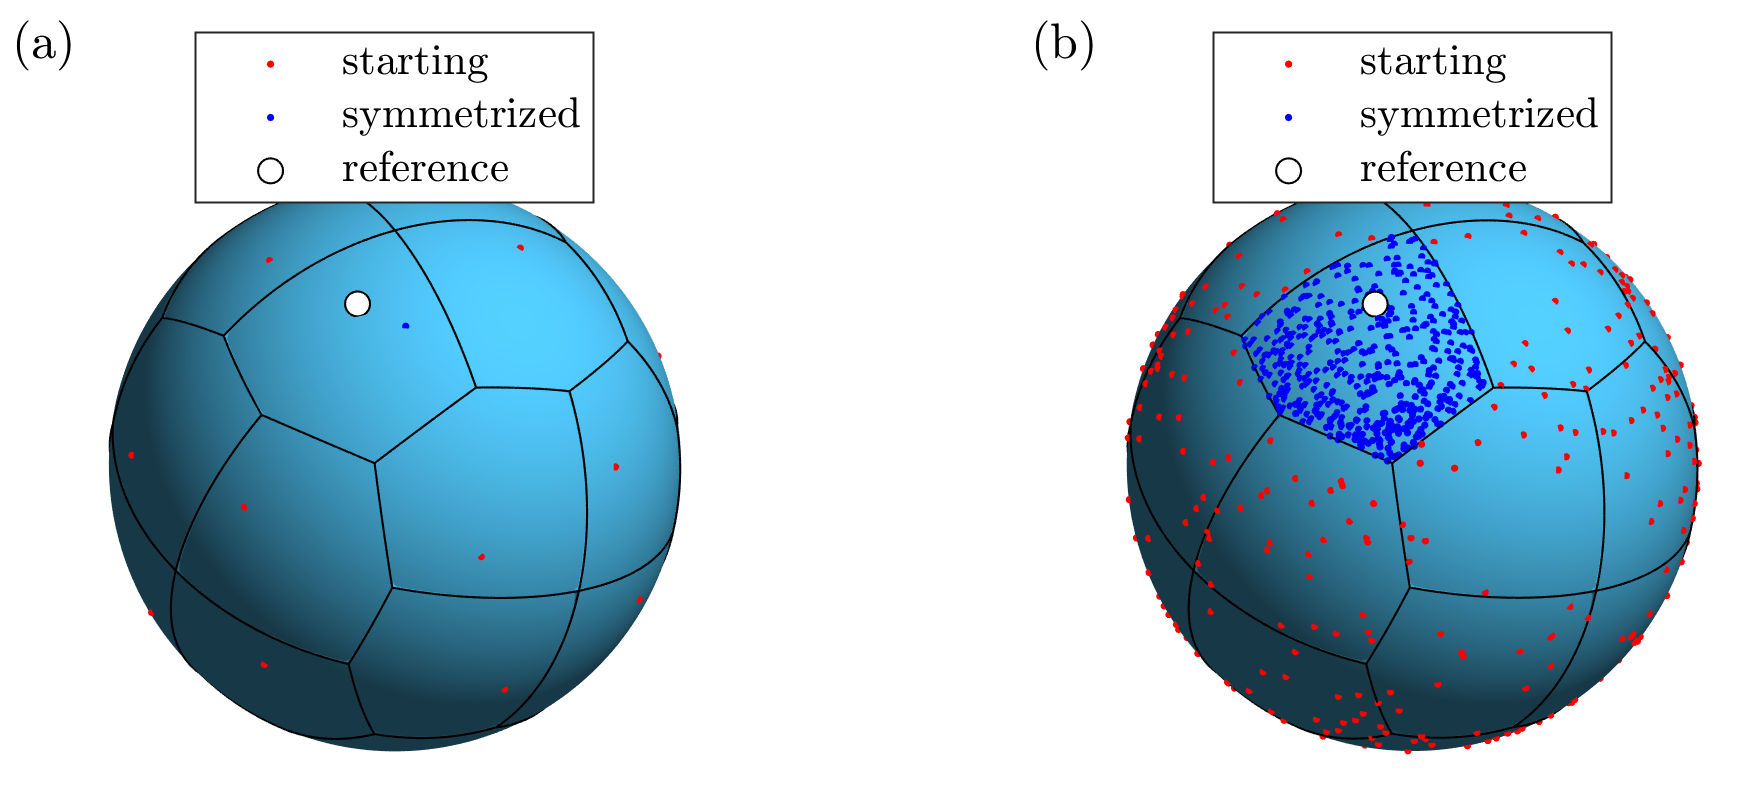
\includegraphics[scale=1]{voronoi.png}
%     \caption{(a) Symmetrization of many points relative to a fixed reference point (white circle) into a 3D Cartesian \gls{vfz} point set (dark blue points). (b) To further illustrate, identical representations of a single input point (magenta points) is symmetrized (dark blue point) relative to a fixed reference point (white circle), demonstrating that only one symmetrized point is found within the borders (black lines) of each of the Voronoi cells (light blue spherical triangle). In the case of \glspl{vfzgbo}, the same procedure applies to the U(1)-symmetrized 6-sphere. Reproduced with permission from Baird, S. G.; Homer, E. R.; Fullwood, D. T.; Johnson, O. K. Computational Materials Science 2021, 200, 110756 \cite{bairdFiveDegreeoffreedomProperty2021}. }
%     \label{fig:voronoi}
% \end{figure*}

%     \subsection{Dimensionality Reduction} \label{sec:methods:dim-reduce}
%     A \gls{svd} transformation is used to remove degenerate dimensions and rotate/align the \gls{vfzgbo} point clouds such that the 1st, 2nd, 3rd, etc. dimensions are progressively smaller.
    
%     Additionally, \gls{pca} is applied and the variance explained by each dimension is extracted.

%     \subsection{Correlation Lengths} \label{sec:methods:correlation}
%     We use semivariogram and numerical optimization methods to obtain several estimates of correlation lengths ($l$) from \gls{vfzgbo} pairwise distances and \glspl{gbe} for two \gls{gb} datasets \cref{sec:methods:litdata}.
    
%     In the semivariogram method, we assume a stationary Gaussian kernel and limit the semivariogram to half of the maximum pairwise distance. We use a correlation strength of $\rho = 0.61$ for correlation lengths reported in this work; however, as the choice of correlation strength is arbitrary, one can use \cref{eq:generalizedcorrelationlength} to determine the length scale corresponding to any specified correlation strength. See \cref{sec:supp:semivariogram} for additional information.
    
%     In a separate method for estimating the correlation length, numerical optimization is performed via gradient-descent-based maximization of a likelihood function that depends on the correlation length, $l$, and noise , $\sigma$, parameters \cite{ExactGPRMethod}.
    
%     % The construction of \gls{gpr} models involves the combination of a prior distribution over the model space, with some set of observations and their quantified uncertainty. The result is a posterior distribution that provides the probability (density) of any particular model in light of the observed data and priors. In \gls{gpr}, as the name suggests, the priors are assumed to be Gaussian and therefore of the form
%     % \begin{equation}
%     %     f\!\left(\mathbf{m}\right) \propto \exp{\left(-\frac{1}{2} {\left(\mathbf{m}-\mathbf{m}_0\right)}^{\mathsf{T}} \mathbf{C}_{\mathbf{m}_0}^{-1} {\left(\mathbf{m}-\mathbf{m}_0\right)}\right)}
%     % \end{equation}
%     % where $f\!\left(\mathbf{m}\right)$ is the probability density of an arbitrary model, $\mathbf{m} = \mathbf{m}\!\left(x\right)$, and $\mathbf{m}_0 = \mathbf{m}_0\!\left(x\right)$ is the prior model (i.e. a guess as to what the true model ought to look like). The quantity $\mathbf{C}_{\mathbf{m}_0} = \mathbf{C}_{\mathbf{m}_0}\!\left(x_i,x_j\right)$ is the "kernel" or covariance function of the prior and it describes the prior (assumed) covariance between the values $\mathbf{m}\!\left(x_i\right)$ and $\mathbf{m}\!\left(x_j\right)$.
    
%     % It is possible to use a wide variety of kernel types, depending on the prior information one may have about the physical phenomenon one is attempting to model, e.g. continuity, differentiability, anisotropy, stationarity, and length-scales of correlation. One of the most common kernels employed is the Gaussian (sometimes called the squared exponential) kernel:
%     % \begin{equation} \label{eq:squared-exponential}                                                                                                                  σ  and σ , and \gls{vfz} coordinates, respectively.
	\left.\text{k[}x_i,x_j\text{$|\theta $]=}\sigma _f{}^2\text{Exp[-}\frac{1}{2}\frac{\left(x_i-x_j\right)\mathsf{T}\left(x_i-x_j\right)}{\sigma _l{}^2}\right]      f       l
\end{equation}
where $\sigma _f$, $\sigma _l$, $\theta$, and $x$ represent signal standard deviation, length scale (i.e. correlation length), unconstrained parameterization of 
    
%     % % estimate $\sigma$ and $l$ from the data.
%     % The values of $\sigma$ and $l$ are typically estimated from the data. One approach, employed by the \texttt{fitrgp()} routine in MATLAB involves numerical optimization via gradient descent which maximizes the likelihood as a function of these parameters \cite{ExactGPRMethod}.
    
%     % % or estimate using empirical semivariograms with a stationary Gaussian kernel.
%     % An alternative approach, adapted from geostatistical applications, involves calculation of the empirical semivariogram [REF], in which one bins the space of pairwise distances between all \glspl{gb} and then calculates half the average pairwise variance of the corresponding property values in each bin:
%     % \begin{equation}
%     %     \label{eq:semivariogram}
%     %     \kappa\!\left(d_k\right) = \frac{1}{2N_k} \sum_{\substack{d_\Omega\left(x_i,x_j\right) \in \\ \left[d_k^-,d_k^+\right]}} {\left| E\!\left(x_i\right) - E\!\left(x_j\right)\right|}^2
%     % \end{equation}
%     % where $x_i$ and $x_j$ are the crystallographic coordinates of \glspl{gb} $i$ and $j$, $d_\Omega\left(x_i,x_j\right)$ is the distance between them, and $E\!\left(x_i\right)$ and $E\!\left(x_i\right)$ are their respective energies. $d_k$ is the location (distance) of the $k$-th bin center having left- and right-hand limits $d_k^-$ and $d_k^+$, and $N_k$ is the number of measurement pairs whose distance falls in the $k$-th bin. Due to limited sampling of large distances and the fact that the most informative part of the semivariogram is the region near $d_k = 0$, it is customary to limit the semivariogram to half of the maximum distance [REF]. The empirical semivariogram is then fit with an analytical model to obtain the parameters of the kernel (covariance) function taking advantage of the relationship
%     % \begin{equation}
%     %     \label{eq:analyticalsemivariogrammodel}
%     %     \kappa\!\left(d\right) = \sigma_f^2 - \mathbf{C}_{\mathbf{m}_0}\!\left(d\right)
%     % \end{equation}
%     % where we have made explicit the stationarity of the Gaussian kernel (i.e. that it depends only the distance between two points, not on their respective locations).
    
%     % % choice of correlation strength
%     % Having obtained a value for the length scale kernel parameter $l$, one can define a correlation length for the data. If the distance between two points is equal to $l$ the kernel function indicates that their correlation will be equal to $\rho = \exp{\left(-1/2\right)} \approx 0.61$. However, one might reasonably want to know the length scale over which \gls{gb} properties are correlated by a different amount. In general for a specified correlation strength, $\rho$, the corresponding correlation length is given by
%     % \begin{equation}
%     %     \label{eq:generalizedcorrelationlength}
%     %     l'\!\left(\rho\right) = l \sqrt{-2 \ln{\rho}}
%     % \end{equation}
%     % We will refer to the parameter $l$ as \emph{the} correlation length, but one can use \cref{eq:generalizedcorrelationlength} to determine the length scale corresponding to any specified correlation strength. %1-2 paragraphs
    
% 	\subsection{Visualizing \glsentrytitlecase{5dof}{short} Paths} \label{sec:methods:path}
% 	geodesic paths between two \glspl{gb} in a \gls{vfz} are obtained via coordinate interpolation constrained to a hyperspherical arc. The geodesic path in a \gls{vfz} is not always the minimum distance path (which may cross the borders of a \gls{vfz}). However, it is instructive to observe these paths because the minimum distance path in \gls{5dof} space is not necessarily the path a \gls{gb} will take during grain growth.
	
% 	\subsection{Literature Datasets}
% 	\label{sec:methods:litdata}
% 	Ni \cite{olmstedSurveyComputedGrain2009a} and Fe \cite{kimPhasefieldModeling3D2014} \gls{gbe} datasets from the literature are used. Intrinsic uncertainty for the Fe simulation data is estimated by the following steps:
% 	\begin{enumerate}
% 	    \item Sort \glspl{gb} into degenerate sets
% 	    \item Determine the average \gls{gbe} for each degenerate set
% 	    \item Compare each of the degenerate \glspl{gb} to the set-wise average \gls{gbe} (\gls{rmse} or \gls{mae})
% 	\end{enumerate}
% 	See \cref{sec:supp:kim-interp:quality} for further details on the methods used to estimate the intrinsic uncertainty of the Fe simulation dataset.
	
	\section{Results and Discussion} \label{sec:results}

    Measuring and/or calculating the properties of \glspl{gb} are generally time-intensive efforts. When seeking to collect data to establish a \gls{gb} structure-property model, it is therefore desirable to determine the minimum number of measurements/calculations needed. To answer this question, three pieces of information are necessary: (1) the size and shape of the space, (2) how close the points must be to one another, and (3) the uncertainty of the data.
    
    To obtain the first piece of information, we need to determine the size and shape of a \gls{vfz}. To obtain the second piece of information, we need to determine the distance over which the property of interest is correlated. If the crystallographic distance between \glspl{nn} in a collection of \glspl{gb} is larger than the correlation length, then there will be large gaps between points where predictions/interpolation will be unreliable. If, on the other hand, the \gls{nn} distances are smaller than the correlation length, then predictions between the measured/calculated values can be expected to be reasonable. Finally, estimates of uncertainty can be obtained by comparing the distribution of repeated measurements. We use \glspl{vfzgbo} to explore structure-property relations in the \gls{5dof} space of \glspl{gb}. To make our aims more complete, we summarize these points in the following questions:
	\begin{itemize}
		\item How large is a \gls{5dof} fundamental zone? What is it shaped like? (\cref{sec:results:dimensions})
		\item How similar are the energies for \glspl{gb} with similar crystallographic character (i.e. how correlated)? How close/densely spaced are randomly generated \glspl{gb}? (\cref{sec:results:correlation})
		\item What is the uncertainty of \gls{ms} simulations of \gls{gb} energy? (\cref{sec:results:error}) %non-globally-optimized \gls{ms} simulations relative to the global minimum \gls{gbe}?
		\item What can crystallographic paths in \gls{5dof} space teach us about material behavior? (\cref{sec:results:paths})
	\end{itemize}
	
	Finally, we discuss the potential for computing numerical derivatives with respect to \gls{5dof} space for computing minimum energy paths and finding local minima (\cref{sec:results:deriv}).
	
	%followed by discussion of potential to use numerical derivatives and identify local minima (\cref{sec:results:vis:apps}).
	
	\subsection{The Size and Shape of an $O_h$ \glsentrytitlecase{vfz}{short}} \label{sec:results:dimensions}
	As described in \cref{sec:methods:vfz}, a \gls{vfz} is defined entirely by the crystallographic symmetries of the material under investigation and the chosen reference point. As such, the size and shape of a \gls{vfz} (and everything else about it) is entirely independent of any GB property that may be evaluated over it.
	
	To investigate the size and shape of a \gls{vfz} for crystals possessing $O_h$ point group symmetry, we applied principal component analysis to the coordinates of a dense \gls{vfz} point set\footnote{This \gls{vfz} point set was used to analyze the \gls{vfz} dimensions and is distinct from (though statistically similar to) the \gls{vfz} point sets used for the Ni and Fe datasets described later.} containing 50,000 points (GBs).
	
	The maximum diameter (largest pairwise distance between points) of this \gls{vfz} was found to be \SI{\sim68.5}{\tobydeg}. If one considers the shortest path between points, including their symmetric images (which may inhabit a neighboring \gls{vfz} image), the maximum pairwise distance is \minsymdist{}.
	
	The principal component dimension of greatest magnitude was found to be \dimOne{}. The sizes of this first and the remaining 7 principal component dimensions are given in \cref{tab:pca-size}. It is interesting to note that the maximum disorientation angle for cubic crystals is \SI{\sim62.8}{\misodeg}, which is comparable to \SI{\sim31.4}{\tobydeg} and therefore represents a distance of a little less than half of the diameter of the \gls{vfz}. These measures of the size of the \gls{vfz} also provide a point of reference against which to compare GB correlation lengths, as will be discussed later.
	
	\begin{table}[!htb]
	    \centering
    	    \caption{Size of \gls{vfz} in each respective PCA dimension for a set of \num{20000} \glspl{vfzgbo}.}
    	    \label{tab:pca-size}
        	\csvautobooktabular[
        	table head={\toprule Dimension & \SI{}{\tobydeg} \\\midrule}]{tables/svd-size.csv}
	\end{table}
	%
	%We also find that the largest minimum (i.e. symmetrized) distance (with a \gls{vfz} ensemble set size of 20 \cite{bairdFiveDegreeofFreedomPropertyUnderReview}) between any two \glspl{gb} in a set of \num{20000} \glspl{gb} is \minsymdist{}.
	%
	The first five \gls{vfz} principal component dimensions are much larger than the last three. In fact, we find that \percExplained{} of the variance (spatial dispersion) is explained by the first 5 PCA transformed coordinates as shown in \cref{tab:pca-explained}. This suggests that the $O_h$ \gls{vfz} inhabits a nominally five-dimensional sub-manifold of $\mathbb{S}^7$. This is to be expected as the octonion parameterization contains redundant dimensions [REF] and reflects the fact that the GB character space is, in reality, five-dimensional.
	
	\begin{table}[!htb]
	    \centering
    	    \caption{Dimension of \gls{pca} transformed coordinates (Dimension) and percent variance explained ($v$) for a set of \num{50000} \glspl{vfzgbo}. The first 5 dimensions cumulatively explain \percExplained{} of the variance. }
    	    \label{tab:pca-explained}
        	\csvautobooktabular[
        	table head={\toprule Dimension & $v$ (\SI{}{\percent}) \\\midrule}]{tables/pca-explained.csv}
	\end{table}	
	
	While examining the diameter and largest dimension of the \gls{vfz} help to characterize its size, consideration of the relative sizes of the principal dimensions of the \gls{vfz} provide an indication of its shape. What does it mean that the 5th dimension is \percFiveVsOne{} the size of the 1st dimension? This gives an indication of the shape of the \gls{vfz}. The first 5 dimensions contain essentially all of the information, which is consistent with the fact that there should be only 5 independent crystallographic parameters to describe a \gls{gb}. The fact that these 5 dimensions are of similar size indicates that the \gls{vfz} is roughly isometric and can be thought of as a hyper-rectangle or hyper-ellipse with only minor eccentricity. 
	
	\subsection{GB Energy Landscapes}
	\label{sec:results:GBELandscapes}
	Using the GPR method (\cref{sec:methods:inference}) of the \texttt{interp5DOF} toolbox, we constructed two different GB energy landscapes over the \gls{vfz}: one for Ni and another for Fe. For the Ni GB energy landscape, we take as input data the 388 GBs from \cite{olmstedSurveyComputedGrain2009a}. For the Fe GB energy landscape we use the \SI{17176} GBs from \cite{kimPhasefieldModeling3D2014}. Both are the result of atomistic molecular statics (MS) simulations.
	
% 	These two datasets are different in some important ways. Whereas the Ni dataset consists of a small number of precise (low-noise) calculations of GB energy, the Fe dataset contains a large number of GB energy values containing significant variability. Details on the methods used to process and estimate the intrinsic uncertainty of the Fe simulation dataset are provided in \cref{sec:supp:kim-interp:quality}.
	
	As they inhabit a nine-dimensional space, these GB energy landscapes are intrinsically difficult to visualize. However, we can characterize them in quantitative ways (\cref{sec:results:correlation:global,sec:results:correlation:local,sec:results:density}) and visualize low-dimensional sub-spaces (\cref{sec:results:paths}).
	
% 	\subsubsection{Correlation Lengths} \label{sec:results:correlation}
	
% 	We present global (\cref{sec:results:correlation:global}) and local (\cref{sec:results:correlation:local}) correlations for the Ni and Fe simulation datasets. We then describe how the number of \glspl{gb} in a \gls{vfzgbo} set affects, on average, how close \glspl{gb} are to their \glspl{nn} (\cref{sec:results:density}) in the context of correlation.
	
	\subsubsection{Global Correlation Lengths} \label{sec:results:correlation:global}
	
    % 	1.	The empirical semivariogram shows a change in concavity, which indicates that the correlations are Gaussian in nature.
    \Cref{fig:globalvariogramfits} shows the empirical semivariograms (circular markers) for the Ni and Fe datasets obtained via \cref{eq:semivariogram}, together with the analytical fits (solid lines) of the Gaussian kernel model (\cref{eq:gaussian-kernel,eq:analyticalsemivariogrammodel}). One of the most fundamental observations comes from the shape of the empirical semivariograms, which, importantly, are computed directly from the data and have no assumption of kernel type imposed on them. As mentioned in \cref{sec:methods:kernels-and-correlations}, there are a wide variety of kernels that could be candidates for modeling correlations in different systems. Different kernels are used to capture different types of correlations, and each has a characteristic signature that can be observed in the semivariogram. For example, when a system exhibits exponential-type correlations, the semivariogram manifests this in the form of an exponential convergence towards an asymptotic constant value at long-distances. Linear and power-law type correlations manifest an absence of a long-distance plateau. In the present system, there is a clear change in concavity in the semivariogram, which is a signature of correlations that are Gaussian in nature. Thus, we find that GB energy correlations in these systems (GB energies in Ni and Fe) appear to be of Gaussian character, and should therefore be modeled using Gaussian kernels. Indeed, the good fit of the Gaussian kernel model to the empirical semivariograms further corroborates this observation.
	\begin{figure*}
	    \centering
	    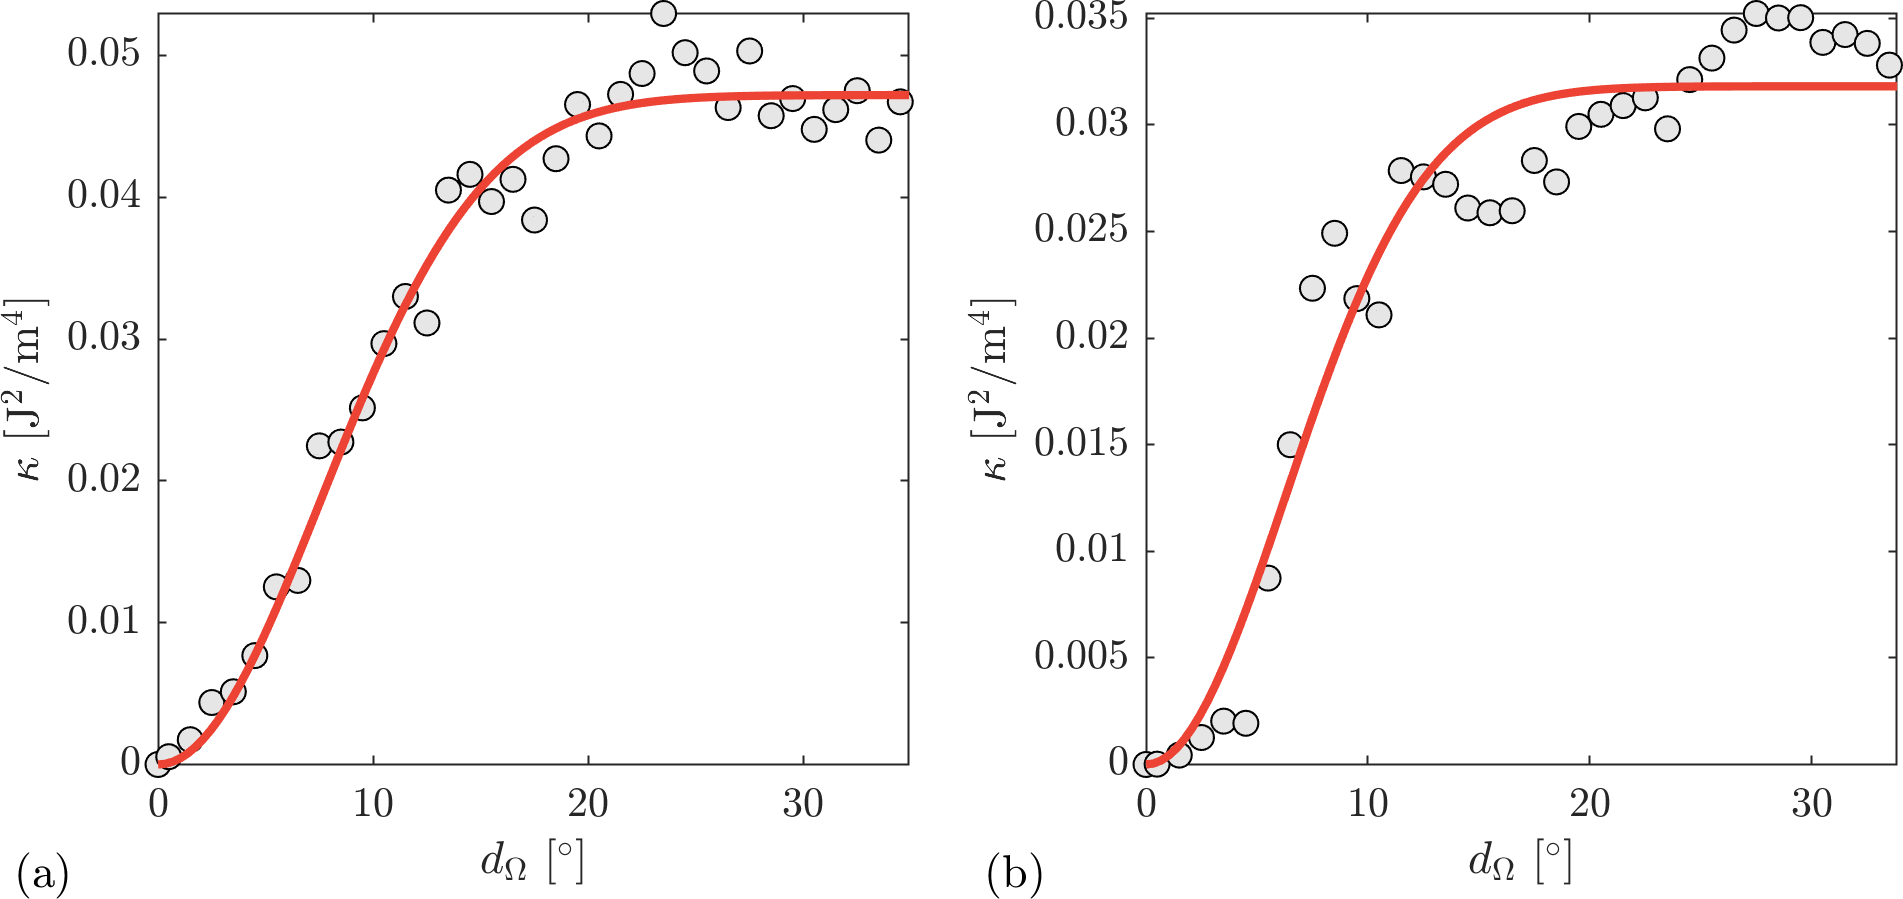
\includegraphics[scale=0.75]{figures/GlobalCorrelationLengthVariograms.png}
	    \caption{Empirical semivariograms (markers) for the (a) Ni and (b) Fe datasets. Solid lines show the fits of the analytical semivariogram models (\cref{eq:analyticalsemivariogrammodel}).}
	    \label{fig:globalvariogramfits}
	\end{figure*}
    
    % 2.	The correlation lengths obtained by fitRGP and the semivariogram method are all around 7.5 oct.deg, which equates to 15 deg, so the 15 deg LAGB/HAGB threshold holds more generally than previously thought.
    In the context of the Gaussian kernel model, GB energy correlation lengths, $l$, were computed for the Ni and Fe datasets using both the semivariogram method (using a bin width of \SI{1}{\tobydeg}) and the maximum likelihood method of \texttt{fitrgp()}. The results are listed in \cref{tab:globalcorrelationlengths} with the annotation ``(Input Data)''.
% 	Using the input data for each of the datasets, global correlation lengths were obtained via the semivariogram method described in \cref{sec:methods:correlation} with a bin width of ${1\ d_{\Omega}^{\circ}}$. \Cref{fig:globalvariogramfits} shows the empirical semivariograms together with the analytical fits used to obtain the values of the respective correlation lengths. The change in concavity suggests that \gls{gbe} correlations for Ni and Fe are Gaussian in nature (\cref{sec:supp:semivariogram:global}).
% 	\begin{figure*}
% 	    \centering
% 	    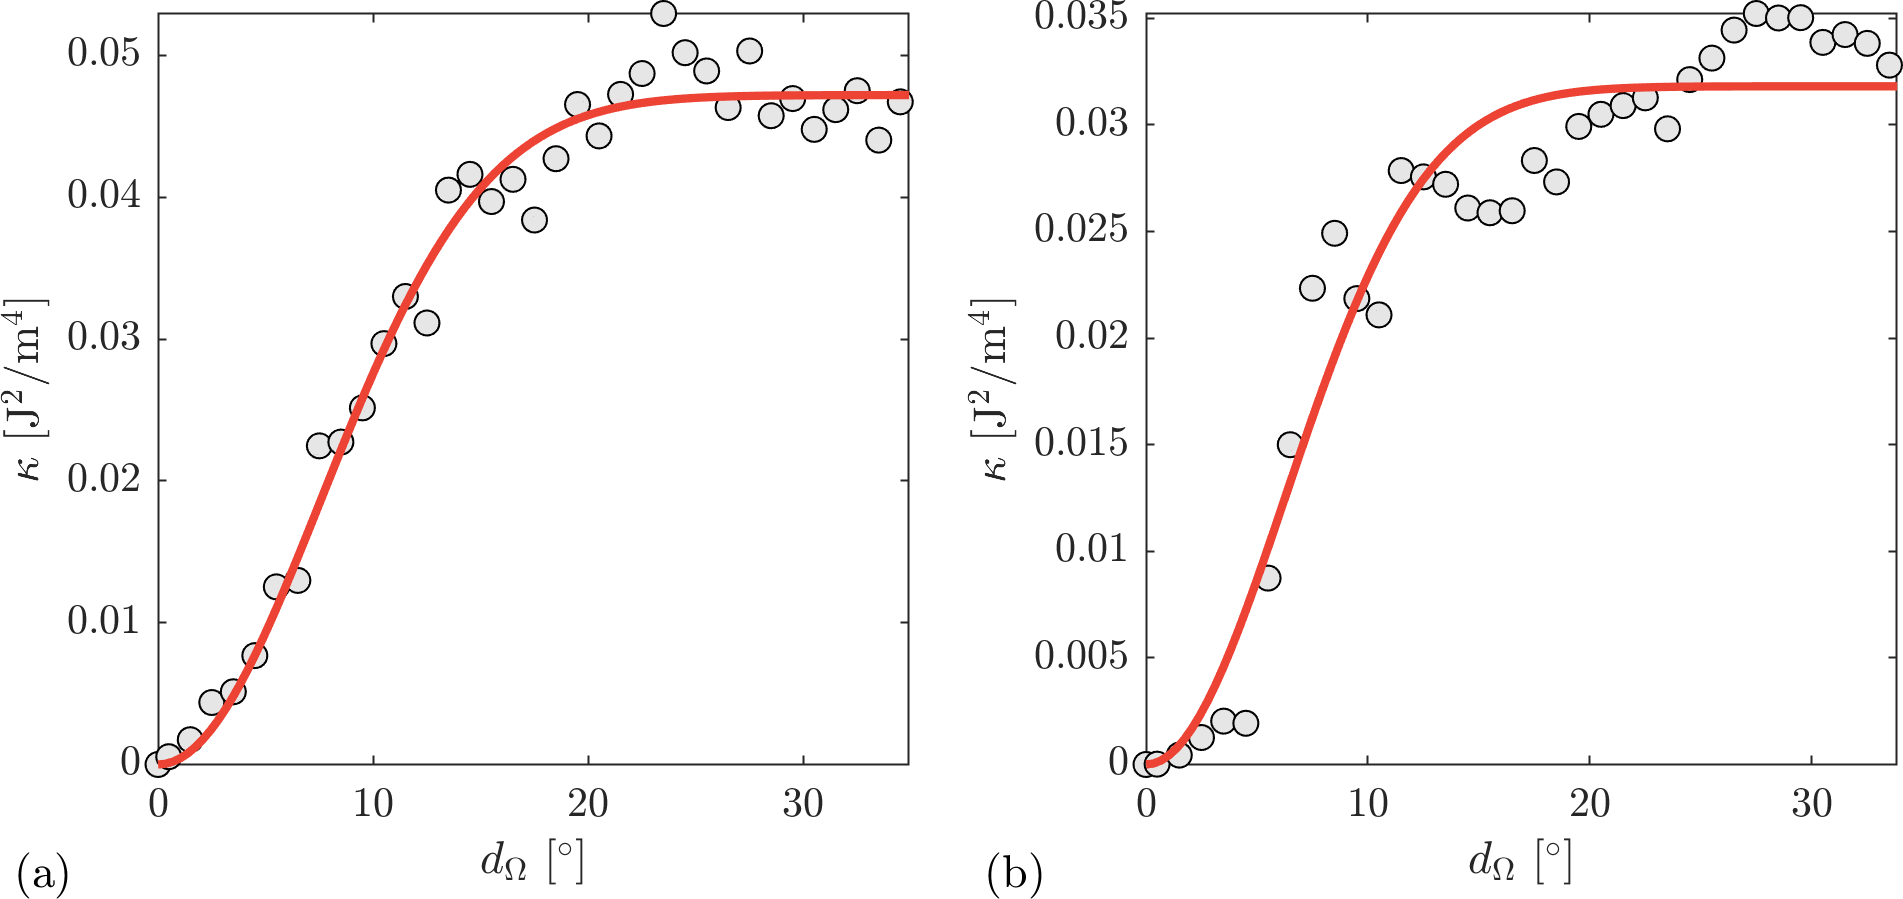
\includegraphics[scale=0.75]{figures/GlobalCorrelationLengthVariograms.png}
% 	    \caption{Empirical semivariograms (markers) for the (a) Ni and (b) Fe datasets. Solid lines show the fits of the analytical semivariogram models (\cref{eq:analyticalsemivariogrammodel}).}
% 	    \label{fig:globalvariogramfits}
% 	\end{figure*}
	
% 	One of the most fundamental observations comes from the shape of the empirical semivariograms. As mentioned in \cref{sec:methods:correlation}, there are a wide variety of kernels that could be candidates for modeling correlations in different systems. Different kernels are used to capture different types of correlations, and each has a characteristic signature that can be observed in the semivariogram. For example, when a system exhibits exponential-type correlations, the semivariogram manifests this in the form of an exponential convergence towards an asymptotic constant value at long-distances. Linear and power-type correlations manifest an absence of a long-distance plateau. In the present system, there is a clear change in concavity in the semivariogram, this is a signature of correlations that are Gaussian in nature. Thus, we find that \gls{gb} energy correlations in these systems are Gaussian, and should therefore be modeled using Gaussian kernels.
	
% 	In addition to the correlation length estimates obtained via the semivariogram method, we also computed correlation length estimates using the gradient-based \texttt{fitrgp()} method described in \cref{sec:methods:correlation}.
	
	We also calculated the correlation lengths exhibited by the GB energy landscapes using the semivariogram method. This was done in two ways: (1) by evaluating the posterior models, $\widetilde{\gamma}\!\left(o\right)$, at the same locations as the input data, and (2) by evaluating the posterior models at randomly selected points (replications of which enabled uncertainty quantification). These results are also listed in \cref{tab:globalcorrelationlengths} with the annotation ``(Posterior Mean at Input/Random Points)''.
	\begin{table*}[]
	    \centering
	    \caption{Correlation lengths obtained via semivariogram and \texttt{fitrgp()} maximum likelihood based approaches in units of \SI{}{\tobydeg}. For the semivariogram of the posterior mean model evaluated at random points, we used $10^3$ random points and repeated this process 10 times. The corresponding values in this table represent the mean $\pm$ one standard deviation of those 10 replicates.}
	    \label{tab:globalcorrelationlengths}
	    \begin{tabular}{l c c}
	    \toprule
	         & \multicolumn{2}{c}{$l: d_\Omega\ [{}^{\circ}]$} \\
	         \cline{2-3}
	         & Ni & Fe \rule{0pt}{2.6ex}\\
	         \midrule
	         Semivariogram (Input Data) & 7.0066 & 6.2591 \\
	         Semivariogram (Posterior Mean at Input Points) & TBD & TBD \\ 
	         Semivariogram (Posterior Mean at Random Points) & $TBD \pm TBD$ & $TBD \pm TBD$ \\
	         \texttt{fitrgp()} Maximum Likelihood (Input Data) & TBD & TBD \\
	         \bottomrule
	    \end{tabular}
	\end{table*}
% 	\begin{table*}[]
% 	    \centering
% 	    \caption{Correlation lengths obtained via semivariogram and \texttt{fitrgp()} maximum likelihood based approaches in units of \SI{}{\tobydeg}. For the semivariogram of the posterior mean model evaluated at random points, we used $10^3$ random points and repeated this process 10 times. The corresponding values in this table represent the mean $\pm$ one standard deviation of those 10 replicates.}
% 	    \label{tab:globalcorrelationlengths}
% 	    \begin{tabular}{l c c}
% 	    \toprule
% 	         & \multicolumn{2}{c}{$l: d_\Omega\ [{}^{\circ}]$} \\
% 	         \cline{2-3}
% 	         & Ni & Fe \rule{0pt}{2.6ex}\\
% 	         \midrule
% 	         Semivariogram (Input Data) & 7.5491 & 6.2665 \\
% 	         Semivariogram (Posterior Mean at Input Points) & 7.7316 & 7.5179 \\ 
% 	         Semivariogram (Posterior Mean at Random Points) & $8.8551 \pm 0.1970$ & $7.7082 \pm 0.1746$ \\
% 	         \texttt{fitrgp()} Maximum Likelihood (Input Data) & 7.3995 & 8.3073 \\
% 	         \bottomrule
% 	    \end{tabular}
% 	\end{table*}
	
	For the Ni dataset, the input data exhibits a correlation length of about \SI{7.5}{\tobydeg} for both the semivariogram and \texttt{fitrgp()} maximum likelihood methods. For the Fe dataset, we observe \SI{6.2665}{\tobydeg} for the semivariogram method and \SI{8.3073}{\tobydeg} for the gradient method, the average of the two being \SI{7.3}{\tobydeg}. Thus both datasets seem to have correlation lengths of about \SI{7.5}{\tobydeg}. 
	
	This is significant. As mentioned previously, for symmetric tilt GBs, the octonion distance metric corresponds to half the difference in misorientation angles ($d_{\Omega} = \Delta\omega/2$). This means that in the more traditional units of degrees of misorientation difference, the observed correlation lengths are very close to \SI{15}{\misodeg}\footnote{We note also that, based on the same Ni data considered in the present work, other authors have suggested GB energies and mobilities are ``well-correlated'' over distances of about \SI{10}{\misodeg} \cite{rohrerComparingCalculatedMeasured2010} and \SI{15}{\misodeg} \cite{olmstedSurveyComputedGrain2009}, respectively. However, these estimates appear to have been primarily qualitative and the degree of correlation was not reported in those works.}, which is the traditional low-angle \gls{gb} threshold\footnote{The traditional low-angle GB threshold is based on the approximate misorientation angle at which dislocation cores in a symmetric tilt GB begin to overlap and, consequently, the dislocation model \cite{readDislocationModelsCrystal1950} begins to break-down \cite{kingWhatDoesIt2006}.}. Thus, the traditional \SI{15}{\misodeg} threshold appears to be applicable (on average) more generally than just for differentiating low- and high-angle GBs. Rather we find that on average, \glspl{gb} that are within \SI{15}{\misodeg} (\SI{7.5}{\tobydeg}) will have well correlated energies ($\rho \geq 0.61$) regardless of their misorientations or \gls{gb} planes (i.e. this threshold is not restricted to symmetric tilt GBs, but holds across the entire \gls{gb} character space).
	
	The correlation lengths obtained by evaluating the GB energy landscapes are similar to those obtained directly from the input data (within about \SI{1}{\tobydeg}), indicating that these GB energy structure-property models correctly reflect the length scale of correlation exhibited by the data.
	
	% 3.	The BRK model has a correlation length of about 10.5 oct.deg. which is about 40% larger than what the data suggests, indicating that the BRK model is overly smooth.
	
	In contrast, if a \gls{gpr} model is trained on a large set of \num{50000} \glspl{gb} sampled from the \gls{brk} model, the numerically optimized correlation length is \SI{10.5}{\degree}, which is about \SI{40}{\percent} larger than what the input data indicates, suggesting that the \gls{brk} model imposes \emph{a priori} information that \glspl{gb} are more correlated than the data warrants. In other words, the \gls{brk} function is too smooth.
	
	% 4.	In the context of the size of the VFZ, these correlation lengths represent about X% of the largest dimension, and Y% of the smallest (non-zero) dimension.
	
	The characterization of the size and shape of the \gls{vfz} presented earlier, allows us to put the observed GB energy correlation lengths into context. In particular, the correlation length of $l = \SI{7.5}{\tobydeg}$ is \SI{\sim11}{\percent} of the diameter of the \gls{vfz}. Or, conversely, the \gls{vfz} is about \SI{9} correlation lengths across.
	
    % 5.	If you vary the correlation strength between 0-1, the corresponding length scale varies from 0-19/23 oct.deg.
	
	As mentioned in \cref{sec:methods:kernels-and-correlations}, the correlation length represents the distance over which GB energy correlations are greater-than-or-equal to $\rho \approx 0.61$. With the aid of \cref{eq:generalizedcorrelationlength} we can determine the length-scale for any correlation strength. Using the correlation lengths, $l$, obtained via the semivariogram of the input data, \cref{fig:correlationlengthvsrho} shows the length scale, $l'$, corresponding to an arbitrary user-specified correlation strength, $\rho$. The length scales over which \gls{gb} energies are correlated range from $l' = \SI{0}{\tobydeg}$ for perfect correlation ($\rho = 1$) to $l' \approx \SI{23}{\tobydeg}$ and $l' \approx \SI{19}{\tobydeg}$ for essentially\footnote{Technically the correlation does not go to exactly zero until the length scale is infinite. The values listed here are for a correlation of $\rho = 0.01$.} zero correlation in the Ni and Fe datasets, respectively.
	\begin{figure}
	    \centering
	    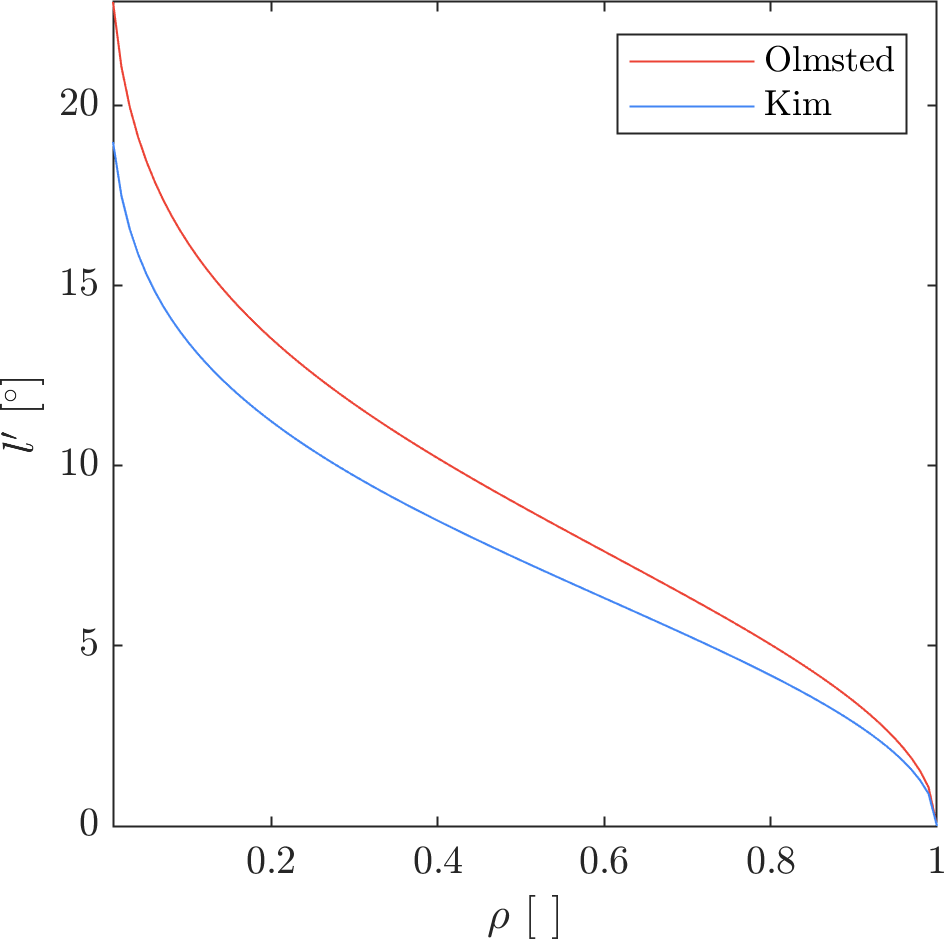
\includegraphics[scale=1]{figures/CorrelationLengthVsRho.png}
	    \caption{Global length scale of correlation, $l'$, in units of \gls{gbo} distance ($d_\Omega\ [{}^{\circ}]$) as a function of correlation strength, $\rho$, for the Ni (\citet{olmstedSurveyComputedGrain2009a}) and Fe (\citet{kimPhasefieldModeling3D2014}) datasets. Multiply \gls{gbo} distance by 2 to convert to units of misorientation angle.}
	    \label{fig:correlationlengthvsrho}
	\end{figure}
	
% 	\begin{table}[]
% 	\centering
% 	\caption{Fitted parameters for two \gls{gpr} models fitted to the 388 simulated Ni \glspl{gbe} by \citet{olmstedSurveyComputedGrain2009a} and fitted parameters for a \gls{gpr} model trained on 80\% of the Fe simulation data (\num{46883} \glspl{gb}). The first Ni model allows $\sigma$ to vary, whereas the second constrains $\sigma$ to be fixed. Mat., $\sigma_L$, $\sigma_F$, $\beta$, and $\sigma$ are the material (i.e. element), kernel length scale in units of $d_{\Omega}$ ($^\circ{}$), signal standard deviation ($J m^{-2}$), constant basis function ($J m^{-2}$), and input property standard deviation ($J m^{-2}$), respectively. %and a \gls{gpr} model trained on \num{50000} \gls{brk} model \glspl{gbe} are shown [NEED TO ADD].
% 	}
% 	\label{tab:resubloss-ni-pars}
% 	\csvautobooktabular[table head={\toprule Mat. & Fix $\sigma$ & $\sigma_L$ ($^\circ{}$) & $\sigma_F$ & $\beta$ & $\sigma$ \\\midrule}]{tables/resubloss-ni-pars.csv}
%     \end{table}
    
    % 	\subsubsection{Global Correlation Length} \label{sec:discuss:correlation:global}
% 	The two simulation datasets have distinct differences from each other, as summarized in \cref{tab:sim-compare}.
% 	\begin{table}[htb!]
% 	    \centering
% 	    \caption{Comparison of Ni (\citet{olmstedSurveyComputedGrain2009a}) and Fe (\citet{kimPhasefieldModeling3D2014}) \gls{ms} simulation datasets. The differences in noise-levels results from whether multiple initial starting configurations were probed in search of a globally minimized configuration as opposed to using a single metastable configuration. }
% \label{tab:sim-compare}
%         \csvautobooktabular{tables/sim-compare.csv}
% 	\end{table}
	
% 	Despite these differences in terms of noise, dataset size, and crystal symmetry, it is interesting to see that the correlation lengths within a \gls{vfz} are similar for the two datasets. Both are lower than the correlation lengths of \SI{10}{\degree} \cite{rohrerComparingCalculatedMeasured2010} and \SI{15}{\degree} \cite{olmstedSurveyComputedGrain2009} previously reported\footnote{Both of these lengths are based on results from \citet{olmstedSurveyComputedGrain2009}.} with respect to misorientation, and are about on par in terms of \gls{bp} normal owing to the fact that \gls{gbo} distances for tilt angles are half the value of misorientation angles.
	
% 	It is reasonable to assume that the Ni data has low noise due to use of a global optimization strategy \cite{olmstedSurveyComputedGrain2009a}; thus, the correlation length of $\sim$\SI{1.9}{\degree} after imposing the low-noise condition suggests that \textit{the Ni dataset may have an actual correlation length much smaller than previously reported.}
	
% 	By contrast, the correlation length of a \gls{gpr} model trained on many \gls{brk} \glspl{gbe} remains relatively large at \SI{10.4}{\degree}. What does this suggest? The \gls{brk} model is smoothed more than the data warrants on its own. This has the following implications:
% 	\begin{enumerate}
% 	    \item More sophisticated methods are required which do not impose mistaken a-priori information about the correlation length\footnote{The a-priori information that the \gls{brk} model imposes is that correlation lengths within a \gls{mfz} or \gls{bpfz} hold for arbitrary paths through \gls{5dof} space and that moving from one subspace to another results in monotonic behavior. }. Instead, the data itself should suggest proper correlation lengths
% 	    \item Larger, low-noise datasets which span all \gls{5dof} are necessary to be confident in structure-property paths that are not restricted to a single \gls{mfz} or \gls{bpfz}
% 	\end{enumerate}
	
% 	We believe that the \gls{gpr} model within the \gls{vfz} framework meets the requirements of point \#1 and is capable of handling the ideal dataset proposed in point \#2.
	
% 	Some questions that remain are:
% 	\begin{itemize}
% 	    \item Does the similarity between correlation lengths for FCC and BCC extend to non-cubic crystal symmetries?
% 	    \item What are the differences in correlation length for other properties? (e.g. mobility)
% 	\end{itemize}
% 	%
% 	It is possible that the correlation length will increase with the size of the \glspl{vfz}, and we expect that the correlation length will depend on the property of interest.
	
	% 6.	Local correlation stuff & Brandon criterion (I think the text for this part is good as is, apart from the minor suggestions noted in my comments in the PDF)
    \subsubsection{Local Correlation Lengths} \label{sec:results:correlation:local}
    
    In addition to the global correlation lengths reported in \cref{sec:results:correlation:global}, we also investigated correlation length scales locally in the vicinity of certain low-$\Sigma$ GBs. This was accomplished by the same semivariogram process explained in \cref{sec:methods:kernels-and-correlations}, except that in \cref{eq:semivariogram} we consider only pairs of \glspl{gb} for which one of the \glspl{gb} is the particular \gls{gb} of interest (i.e. we fix one of the GBs). Because the resulting set of \gls{gb} pairs is smaller than in the global analysis, we use larger bins with a width of \SI{2}{\tobydeg} for the local empirical semivariograms.
    
    \Cref{fig:localvariogramsolmsted,fig:localvariogramskim} show the local empirical semivariograms for the Ni and Fe datasets respectively. Each panel shows the semivariogram centered at a different low-$\Sigma$ GB. While noisier than the global empirical semivariograms, reasonable fits were obtained for all except $\Sigma 5$ in the Ni dataset (see \cref{sec:supp:semivariogram:local}).
    
    % \begin{figure*}
    %     \centering
    %     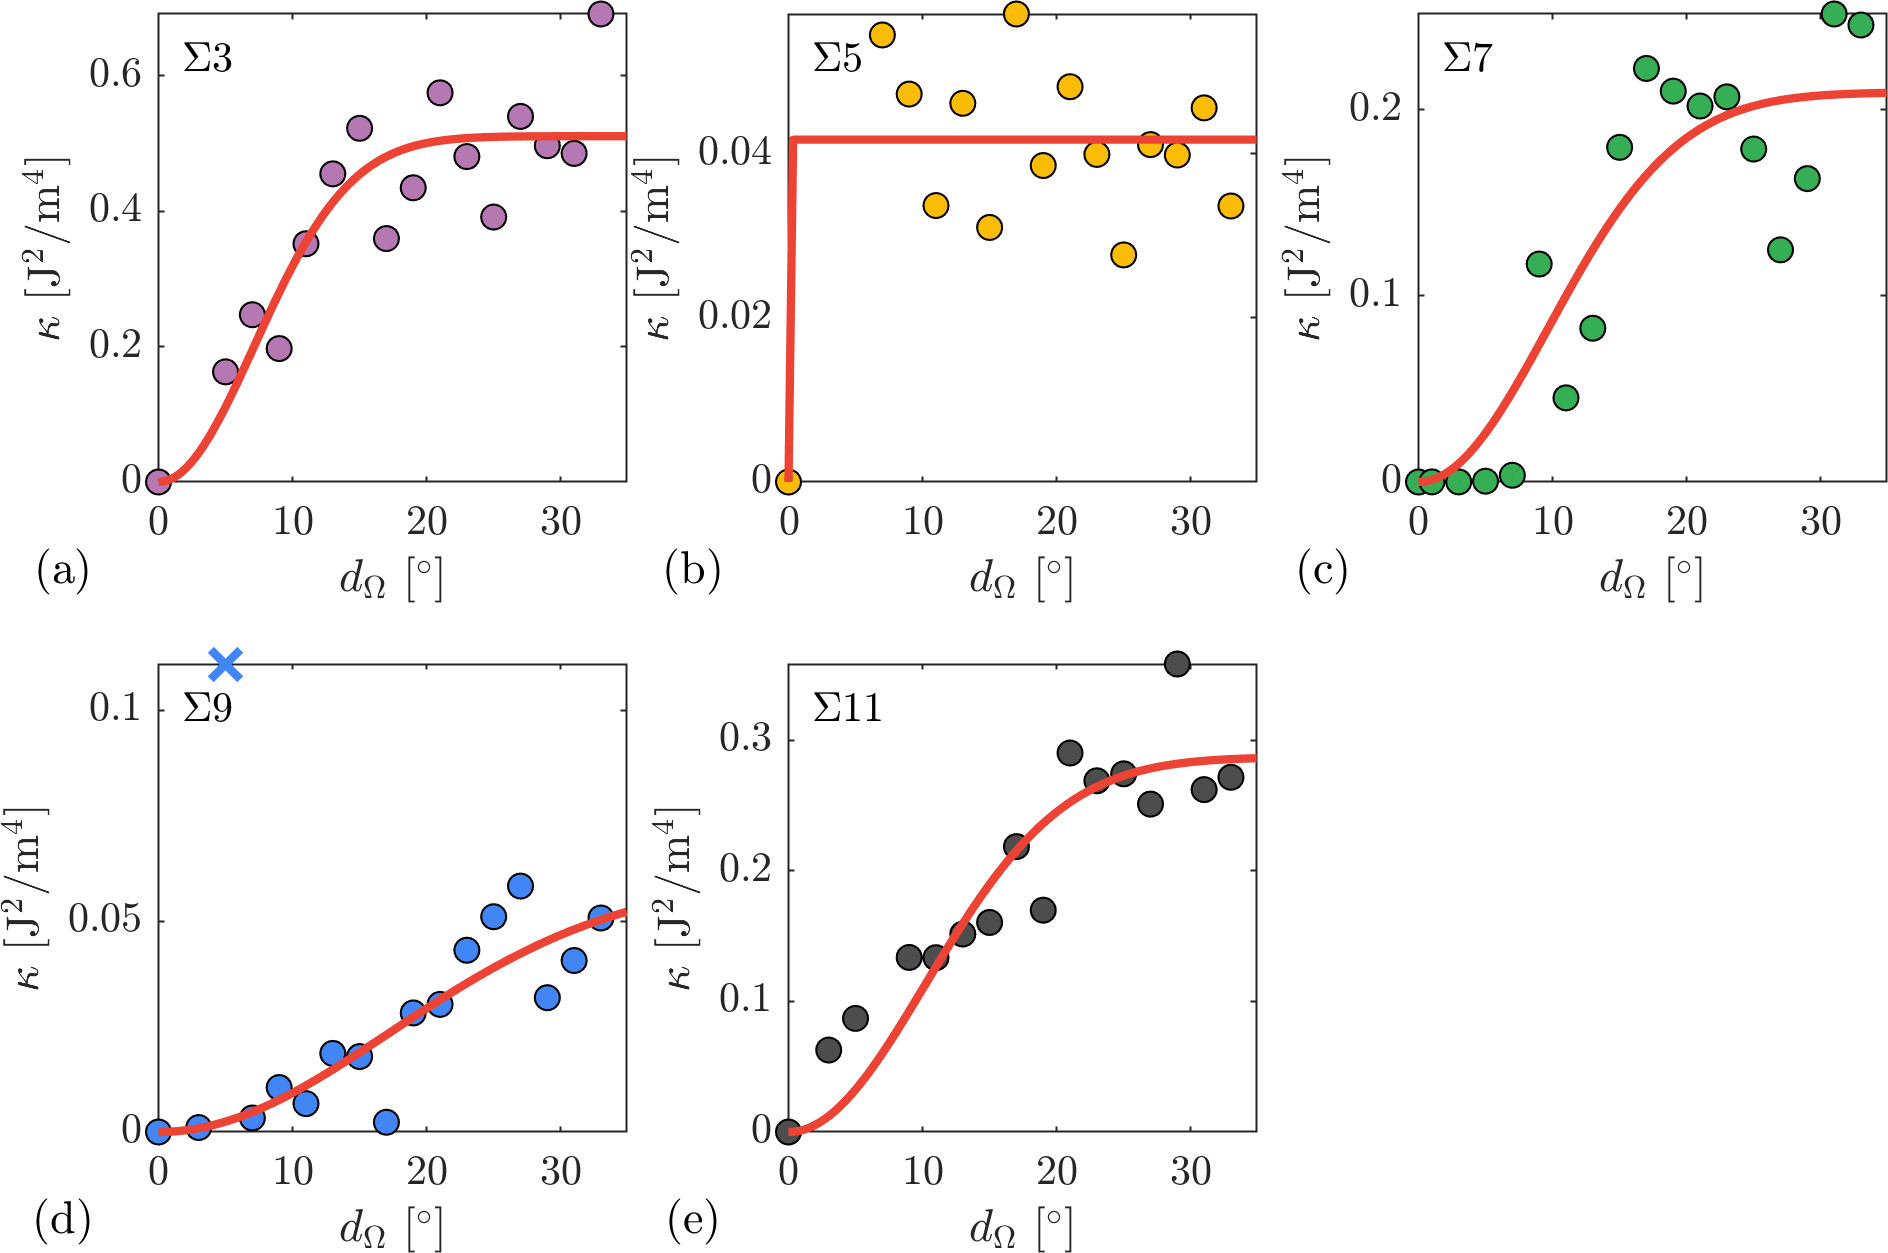
\includegraphics[scale=1]{figures/LocalCorrelationLengthVariogramsOlmsted.png}
    %     \caption{Local empirical semivariograms (markers), respectively centered at various low-$\Sigma$ \glspl{gb} for the Ni dataset. Solid lines show the fits of the analytical semivariogram models. In (d) the one point marked with an $\times$ was considered an outlier and was excluded from the fit.}
    %     \label{fig:localvariogramsolmsted}
    % \end{figure*}
    % \begin{figure*}
    %     \centering
    %     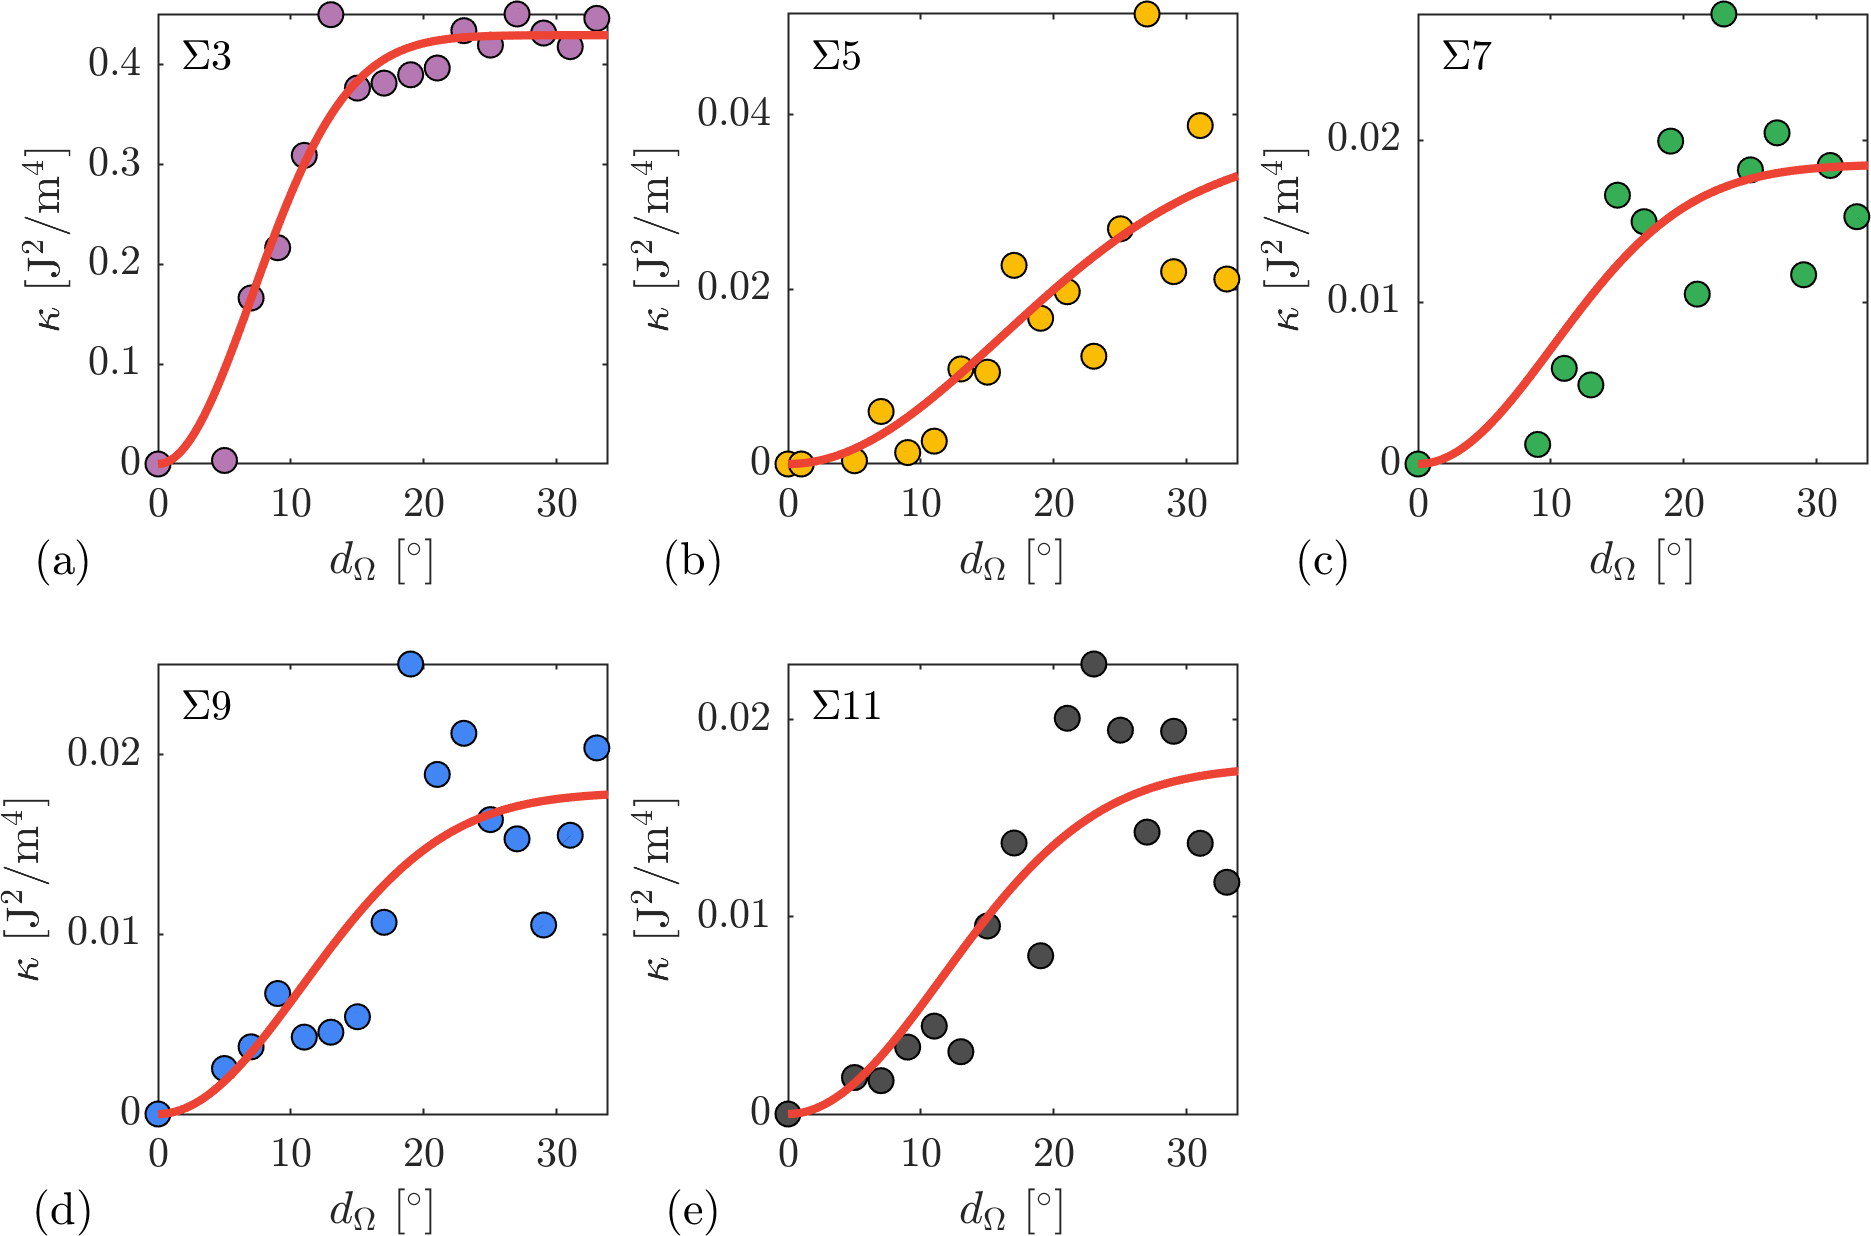
\includegraphics[scale=1]{figures/LocalCorrelationLengthVariogramsKim.png}
    %     \caption{Local empirical semivariograms (markers), respectively centered at various low-$\Sigma$ \glspl{gb} for the Fe dataset. Keys for which \glspl{gb} each of these correspond to in the original papers are given for Fe and Ni in \cref{tab:sigma-key-olmsted,tab:sigma-key-kim}, respectively. Solid lines show the fits of the analytical semivariogram models.}
    %     \label{fig:localvariogramskim}
    % \end{figure*}
    % The local empirical semivariograms are noisier than the global empirical semivariograms, likely due to considering fewer \gls{gb} pairs. Nevertheless, reasonable fits were obtained for most of the \glspl{gb} with the exception of the $\Sigma 5$ \gls{gb} in the Ni dataset. In many of the local semivariograms we again see the signature change in concavity suggesting that the local correlations in the vicinity of these \glspl{gb} are also Gaussian in nature. However, there are some exceptions where the nature of the correlations is more ambiguous. We anticipate that this ambiguity could be resolved with datasets that are either larger (compared to the Ni dataset) or having less noise (compared to the Fe dataset) than those considered here. However, the local empirical semivariograms seem to be generally consistent with Gaussian-type correlations.
    
    \Cref{tab:localcorrelationlengths} provides the local correlation lengths obtained for each of the low-$\Sigma$ \glspl{gb} for each of the datasets. The most noteworthy observation is that these correlation lengths are different from one another and different from the respective global correlation lengths. While the local correlation lengths for the $\Sigma 3$ \glspl{gb} are similar to the global values for both datasets, other \glspl{gb} have correlation lengths more than twice as large as the global correlation length (the $\Sigma9$ in the Ni dataset, and the $\Sigma 5$ in the Fe dataset). The fact that certain local correlation lengths differ from the global correlation length suggests that a non-stationary Gaussian kernel (which depends on both relative distance and absolute location) may be a more appropriate choice than the stationary Gaussian kernel (\cref{sec:supp:semivariogram:local}).
    \begin{table}[]
	    \centering
	    \caption{Local correlation lengths in the vicininty of specific low-$\Sigma$ GBs, obtained via the semivariogram method in units of \SI{}{\tobydeg}. The fit of the $\Sigma 5$ \gls{gb} semivariogram for the Ni dataset was sufficiently poor that we do not report a corresponding correlation length.}
	    \label{tab:localcorrelationlengths}
	    \begin{tabular}{l d{2.4} d{2.4}}
	    \toprule
	         & \multicolumn{2}{c}{$l: d_\Omega\ [{}^{\circ}]$} \\
	         \cline{2-3}
	         & \multicolumn{1}{c}{Ni} & \multicolumn{1}{c}{Fe} \rule{0pt}{2.6ex}\\
	         \midrule
	         $\Sigma 3$ & 7.1460 & 7.0921 \\
	         $\Sigma 5$ & \multicolumn{1}{c}{---} & 16.0440 \\ 
	         $\Sigma 7$ & 9.6533 & 10.1493 \\
	         $\Sigma 9$ & 17.2601 & 10.7792 \\
	         $\Sigma 11$ & 10.2027 & 11.6011 \\
	         \bottomrule
	    \end{tabular}
	\end{table}
	
    % The traditional Gaussian kernel exhibits the property of stationarity, meaning that the covariance depends only on the distance between two points, not on their respective locations (i.e. $\mathbf{C}_{\mathbf{m}_0}\!\left(x_i,x_j\right) = \mathbf{C}_{\mathbf{m}_0}\!\left(d\left(x_i,x_j\right)\right)$). The use of a stationary kernel implies a prior assumption that there is a single global correlation length that applies everywhere. The fact that we observe significant variation in correlation length across the \gls{gb} character space suggests that it would be better to employ non-stationary kernels (this is why, when referring to the global correlation length results presented earlier, we were careful to say that the global correlation lengths hold "on average" across the space). In particular, due to the fact that the local semivariograms do seem to be generally consistent with Gaussian-type correlations, we suggest that the non-stationary version of the Gaussian kernel [REF] may be a reasonable choice. One additional potential benefit of employing non-stationary kernels might be improved resolution of cusps in the \gls{gb} energy landscape.
    
    These local correlation lengths facilitate an interesting comparison with the canonical Brandon criterion \cite{brandonStructureHighangleGrain1966a}. The Brandon criterion provides a threshold for the maximum angular deviation that can be accommodated by a \gls{csl} boundary before losing coincidence:
    \begin{equation}
        \Delta \theta = \theta_0 {\Sigma}^{-1/2}
        \label{eq:brandoncriterion}
    \end{equation}
    where $\Delta \theta$ is the angular deviation threshold, $\theta_0 = \SI{15}{\misodeg}$ is a constant corresponding to the traditional low- to high-angle \gls{gb} threshold and $\Sigma$ is the reciprocal density of coincidence lattice points (i.e. the \gls{csl} number). The Brandon criterion predicts that the amount of distortion that the \gls{gb} can accommodate (e.g. via introduction of \gls{gb} dislocations) before losing coincidence should \emph{decrease} with $\Sigma$ because the density of coincident sites decreases with $\Sigma$.
    
    In contrast, \cref{fig:brandoncriterioncomparison} shows that correlation lengths generally \emph{increase} with $\Sigma$. That is to say that, in general, there is a trend of \gls{gb} energies being correlated over longer length scales with increasing $\Sigma$. This seems reasonable since the deepest cusps in the \gls{gb} energy landscape (which would produce small correlation lengths) tend to correspond to the lowest-$\Sigma$ GBs.
    \begin{figure}
        \centering
        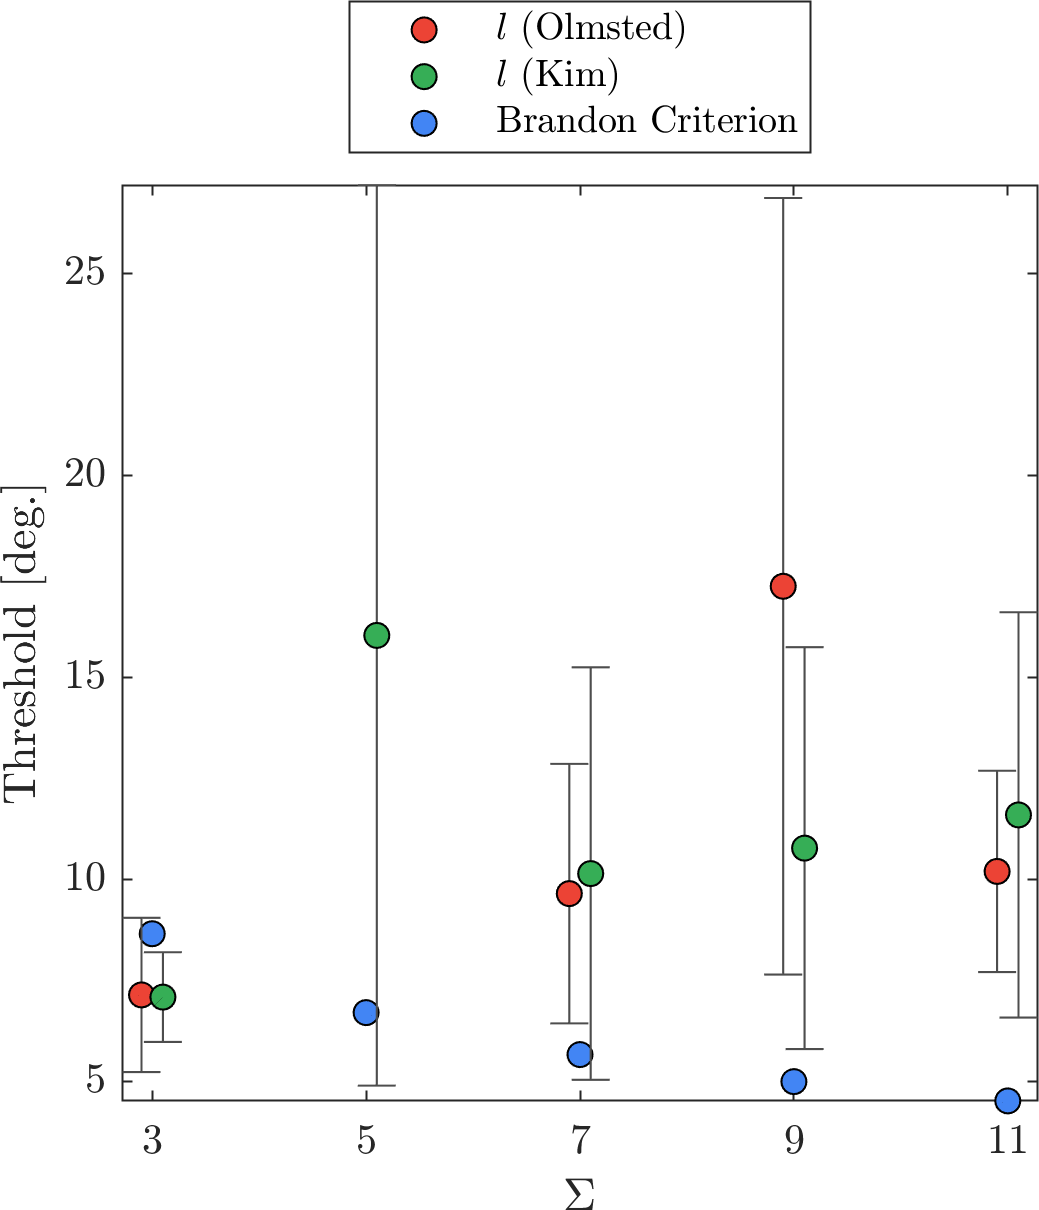
\includegraphics[scale=1]{figures/BrandonCriterionComparison.png}
        \caption{Comparison of the Brandon criterion \cite{brandonStructureHighangleGrain1966a} for low-$\Sigma$ \glspl{gb} (in units of ${}^{\circ}$) to the local correlation lengths obtained in this work (in units of \SI{}{\tobydeg} $d_{\Omega}^{\circ}$). Conversion to consistent units would unnecessarily separate the data without changing the trends, and since we are most interested in the uniqueness of the trends rather than the numerical values themselves, we leave the values in their native units. Error bars indicate 95\% confidence intervals. There is no marker for the $\Sigma 5$ \gls{gb} in the Ni (Olmsted) dataset because of the failure of the fit discussed above.}
        \label{fig:brandoncriterioncomparison}
    \end{figure}
    This suggests that while strict structural coincidence may indeed be lost over smaller crystallographic deviations with increasing $\Sigma$, \gls{gb} energies seem to be relatively insensitive to this loss of coincidence and instead seem to be increasingly correlated over larger length scales. This may explain why previous researchers found $\Sigma$ to be a poor predictor of GB energy \cite{olmstedSurveyComputedGrain2009a}.

	\subsubsection{Density and Distribution of Points in the $O_h$ VFZ} \label{sec:results:density}
	
	Having characterized the size and shape of the \gls{vfz}, and having determined the correlation length for GB energy, we are now in a position to address the question of how many points are necessary to span the space. To answer this question we generate \gls{vfz} point sets of varying cardinalities (number of points in the set), uniformly distributed over the \gls{vfz}, and compute the pairwise distances between points in each respective \gls{vfz} point set.
	
	\Cref{fig:nndist-vs-setsize} illustrates how the average \gls{nn} distance varies with the cardinality of the \gls{vfz} point set. The average \gls{nn} distance ranged between \SI{10.7175 \pm 0.3684}{\tobydeg} and \SI{2.6479 \pm 0.2254}{\tobydeg} for \gls{vfz} point set cardinalities of \num{100} and \num{50000}, respectively. A second vertical axis is also shown to put the \gls{nn} distances in the context of the \SI{7.5}{\tobydeg} correlation length. This suggests that for the average \gls{nn} distance to be less than 1 correlation length, a uniformly distributed \gls{vfz} point set containing at least 534 GBs is required.
	\begin{figure}
		\centering
		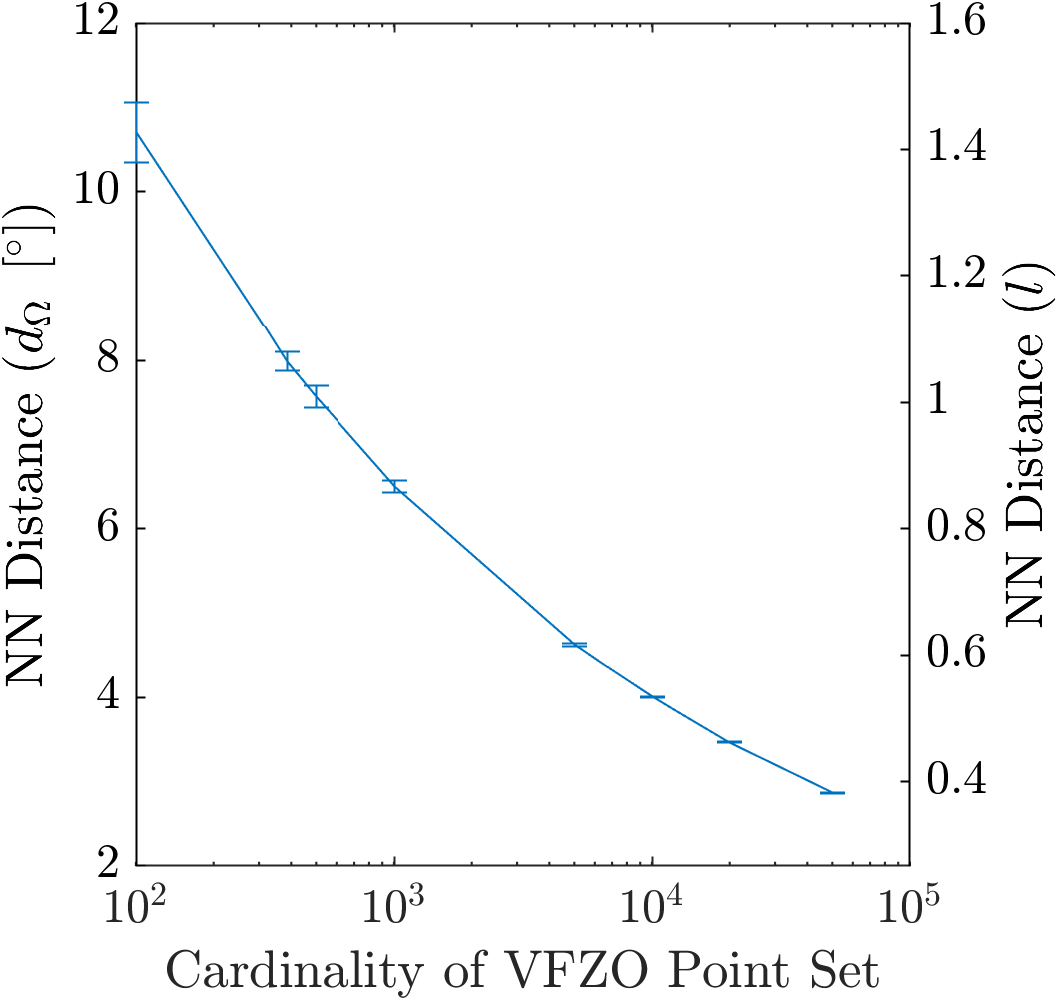
\includegraphics[scale=1]{nndist-vs-setsize-final.png}
		\caption{\Gls{nn} distances (\SI{}{\tobydeg}) vs. the cardinality of the \gls{vfz} point set. Minimum and maximum cardinalities considered were \SI{100} and \SI{50000}, respectively. Each value represents the mean of 70-80 trials with 1 standard deviation error bars shown.}
		\label{fig:nndist-vs-setsize}
	\end{figure}
	
	The Ni and Fe datasets contain \SI{388} and \SI{17176} GBs, which would correspond to average \gls{nn} distances of \SI{\sim8}{\tobydeg} (\SI{1.07} correlation lengths) and \SI{\sim3.6}{\tobydeg} (\SI{0.48} correlation lengths), respectively. However, the GBs in these datsets are not uniformly distributed, and instead exhibit average \gls{nn} distances of \SI{5.27\pm3.54}{\tobydeg} ($0.70\pm0.47$ correlation lengths) and \SI{3.33\pm2.57}{\tobydeg} ($0.44\pm0.34$ correlation lengths), respectively. This indicates that the GBs in these datasets are more tightly clustered than would be expected for a uniform distribution with the same cardinality.
	
	To minimize the uncertainty of predictions, it is desirable to have observation point densities such that there is more than a single \gls{nn} within one correlation length on average. At a minimum, one should have at least $D+1$ points within a correlation length on average, where $D$ is the dimensionality of the space. Such a sampling scheme will mean that points will be surrounded by a $D$-simplex of \glspl{nn} all within one correlation length, on average. Alternatively, a conservative dense sampling approach might require $2^D$ points within a correlation length, on average. For GBs and the nominally 5D \gls{vfz} reported here (see \cref{sec:results:dimensions}) these estimates correspond to a target of having somewhere between \SIrange[range-phrase={--}]{6}{32}{} \glspl{nn} within a correlation length. \Cref{fig:nncontour} shows the number of \glspl{nn} as a function of distance and \gls{vfz} point set cardinality. To obtain at least \SI{6}{} \glspl{nn} within one correlation length on average requires a \gls{vfz} point set containing \SI{22554}{} \glspl{gb}, and to achieve \SI{32}{} \glspl{nn} within one correlation length a \gls{vfz} point set containing \SI{120014}{} \glspl{gb} is required.
	\begin{figure}
		\centering
		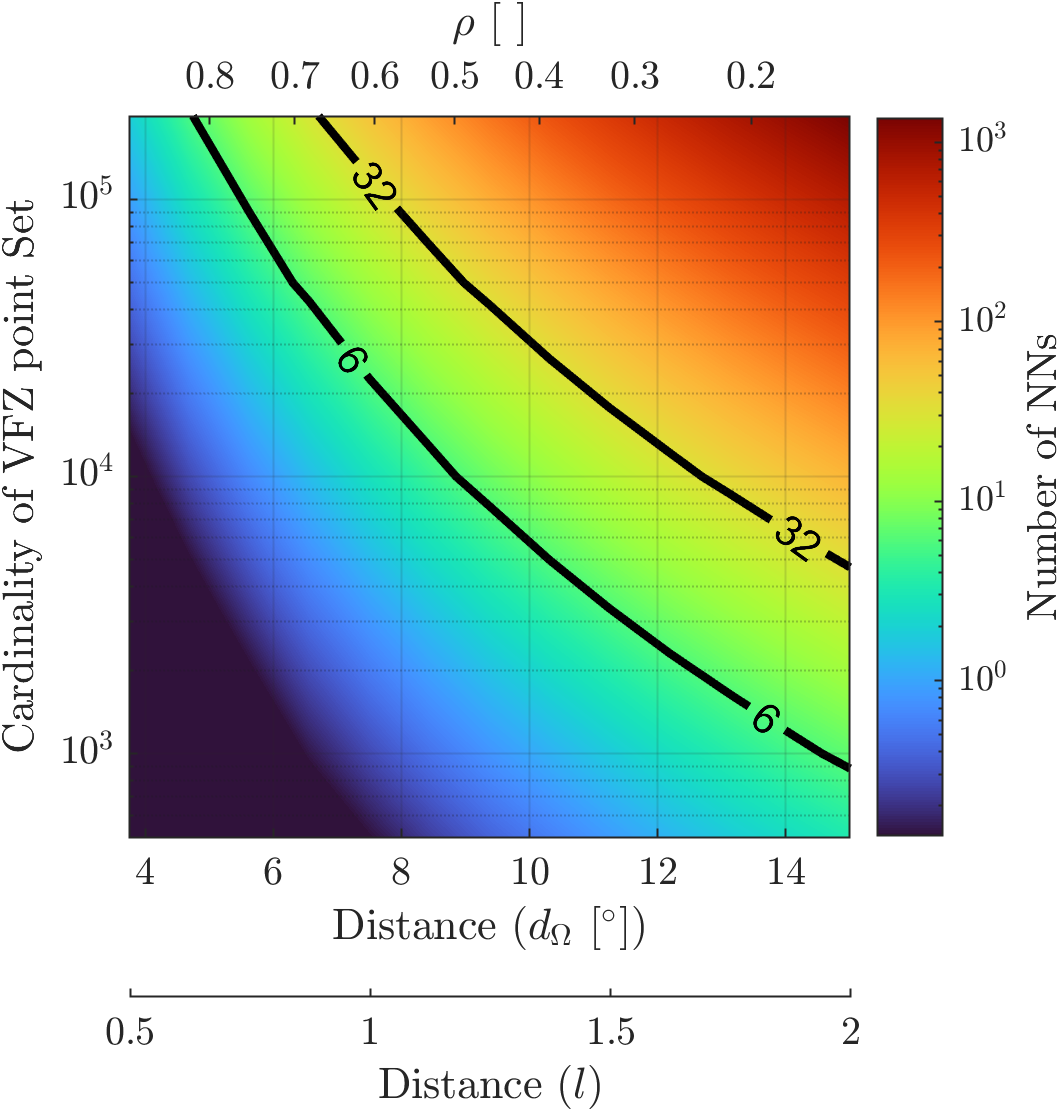
\includegraphics[scale=1]{figures/nncontour.png}
		\caption{Contour plot showing the average number of \glspl{nn} within a specified distance for points in a \gls{vfz} point set as a function of the set cardinality. Values represent the mean of 3 trials. The median (mean) coefficient of variation across all conditions was \SI{0.5853}{} (\SI{1.50}{}). Contours representing $D+1=6$ and $2^D = 32$ are shown. Also indicated are the number of correlation lengths and correlation strengths corresponding to a given distance (for an assumed correlation length of \SI{7.5}{\tobydeg}).}
		\label{fig:nncontour}
	\end{figure}
	
	This is not to say that datasets containing fewer than this number of GB measurements should not be used. However, one should be aware that if the limited measurements are distributed uniformly, the uncertainty of models built from such datasets is likely to be significant, or if the measurements are not distributed uniformly (the more common case if the data come from atomistic simulations), it will vary with position, with predictions for some regions---where points are more tightly clustered---having low uncertainty and predictions for other regions---where points are sparse---having higher uncertainty.
	
	For the Ni and Fe datasets considered here, the expected number of \glspl{nn} if the GBs were distributed uniformly are X and Y, while the actual number of \glspl{nn} are A and B.
	
	It is also useful to consider the implications of this finding for experimental work. Consider a polycrystalline microstructure possessing a uniform orientation distribution function, and grain-growth-type grain morphology. If two serial sections are characterized to determine the full 5D GB character of a single plane, and we consider just one normal (the middle one) from each GB, we find that the resulting points are distributed relatively uniformly, so that ...
	
	For a specific \num{50000} \gls{vfzgbo} set, the \gls{nn} \gls{gbo} distance is \SI{\nnomega{}}{\degree} (\cref{fig:nnhist-knn-50000}a) while the average 100-th \gls{nn} distance is within \SI{10}{\degree} (\cref{fig:nnhist-knn-50000}b). While not shown, we also found that the sampling scheme used in this work (sampling misorientation and \gls{bp} normal as opposed to sampling \glspl{gbo} directly) produced no qualitative differences in the observed distributions.
	
	\begin{figure*}
		\centering
		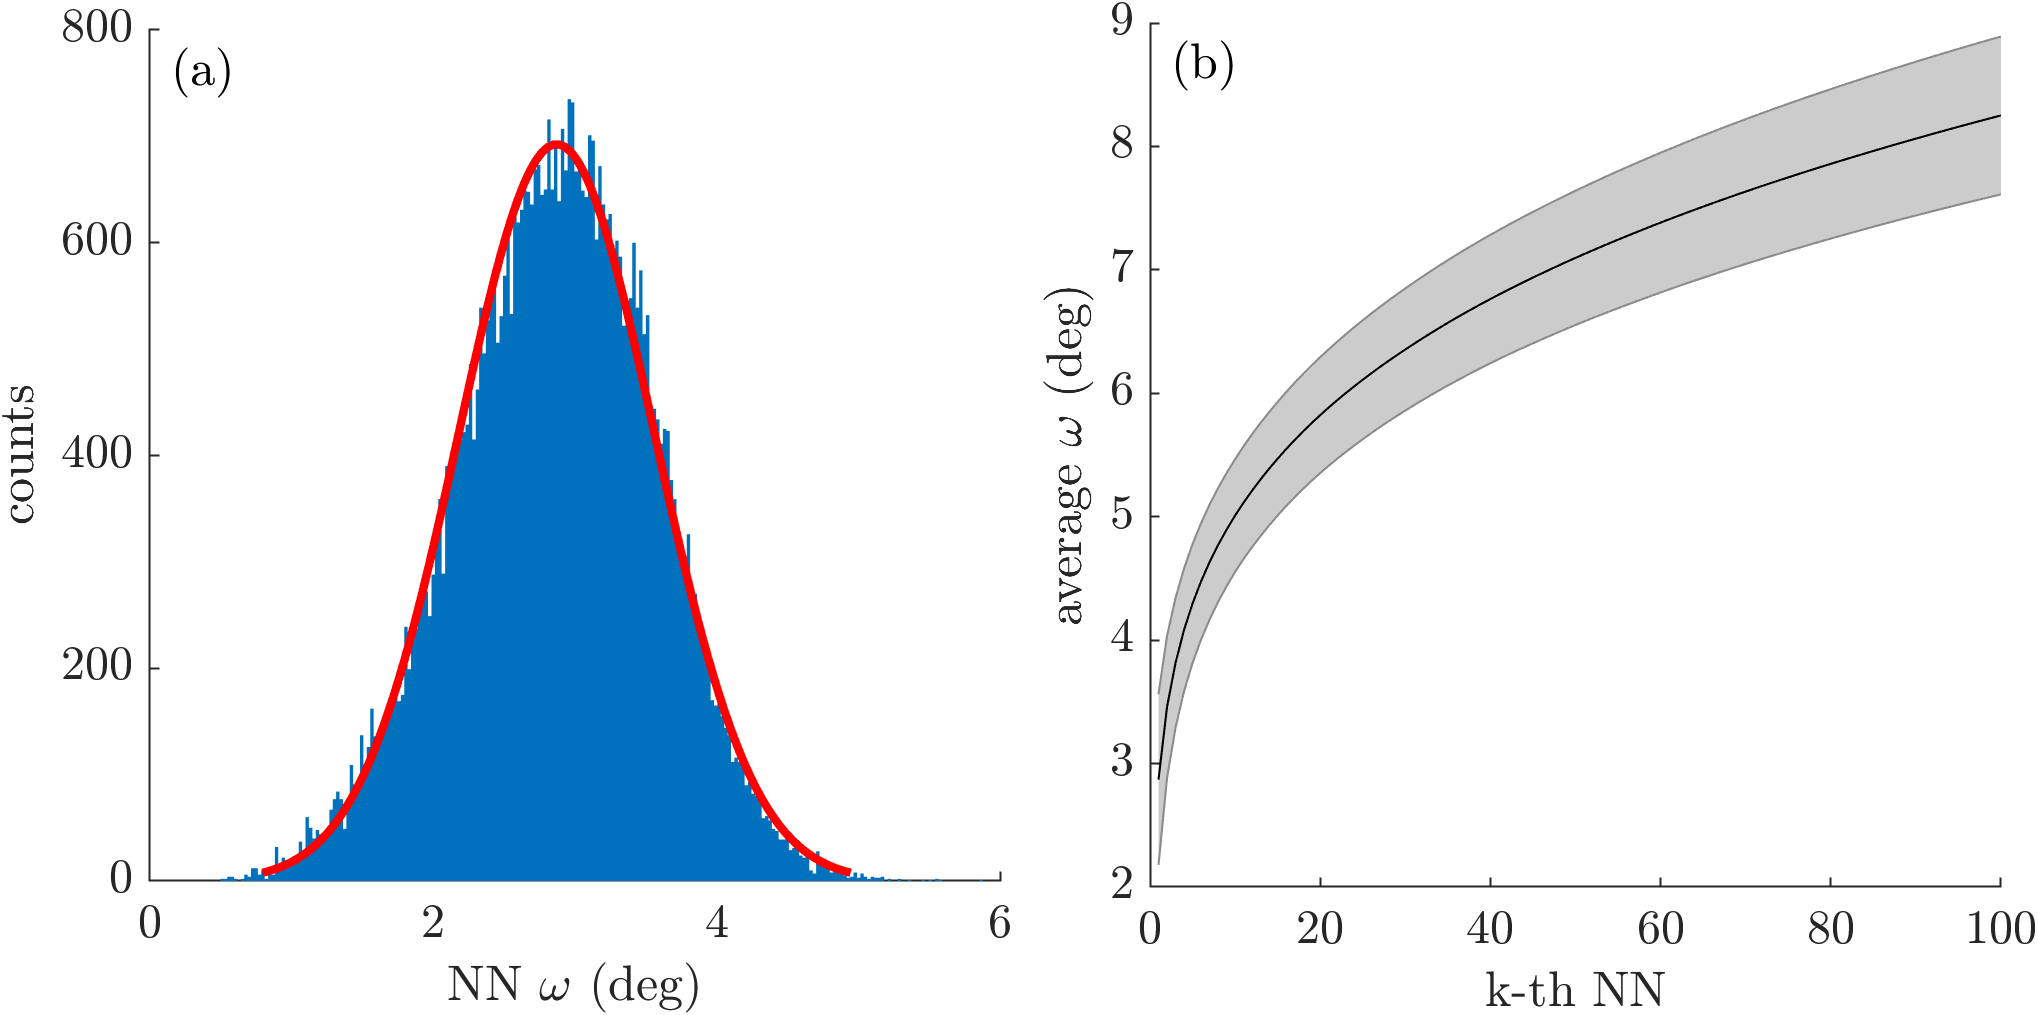
\includegraphics[scale=1]{nnhist-knn-50000.png}
		\caption{(a) Histogram of \gls{nn} \gls{gbo} distances ($d_{\Omega}$) in a \gls{vfzgbo} set of \num{50000} points. The average \gls{nn} distance was \SI{\nnomega}{\degree}. (b) The average k-th nearest neighbor distances demonstrate that \glspl{nn} up to the $\sim$\num{10}-th \gls{nn} fall within a tolerance of $\sim$\SI{5}{\degree}. Standard deviation uncertainty bars using approximately 10 trial runs are also shown. }
		\label{fig:nnhist-knn-50000}
	\end{figure*}
	
	How large is the local region of influence for a \gls{5dof} interpolation model? Another way of phrasing this question is: how many \glspl{gb} are necessary to sample in the space to obtain a model that's accurate enough? \Gls{nn} distances give context to these questions: if \num{50000} \glspl{gb} are randomly sampled, then on average, these \glspl{gb} are \SI{2.6479 \pm 0.2254}{\degree} apart from their \gls{nn}. In the context of correlation lengths of $\sim$\num{7}$-$\SI{8}{\degree} (\cref{sec:results:correlation:global}), a random set of at least $\sim$\num{10000} \glspl{gb} is required to reach a reasonable goal of half the correlation length (i.e. to have a reasonably performing structure-property model). By contrast, A set of \num{388} randomly sampled \glspl{gb} will yield average \gls{nn} distances of $\sim$\SI{7.5}{\degree}. The fact that this is approximately the same as the correlation lengths derived in this work suggest that this size of dataset is far too small. We demonstrate this via an example.
	
	Assume the property of a particular \gls{gb} which has been randomly sampled has never been measured before. What is available, however, is a set of property measurements for \num{388} other \glspl{gb}. Our model suggests that \glspl{gb} which are further apart than $\sim$\SI{7.5}{\degree} can't reveal much information about each other. So, how many \glspl{gb} are in this local region of influence to be able to predict the property for the \gls{gb} of interest? The answer is only one \gls{gb}. To make matters worse, this \gls{gb} happens to be at the borderline distance of containing relevant information (closer is better).
	
	Correlation lengths can vary locally and are subject to some interpretation (\cref{sec:results:correlation:local}); however, it's clear that without knowing more, the property prediction of the \gls{gb} of interest might be OK, or it might be completely off. The \gls{brk} \cite{bulatovGrainBoundaryEnergy2014} model (which uses \num{388} \glspl{gb}) works around this limitation by imposing prior information: a "scaffolding" of \glspl{gb} at high-symmetry cusps is used, and it is assumed that the function varies monotonically from point to point everywhere else. For a well-studied property (\gls{gbe}) and a well-studied material system (FCC), this domain knowledge can be successfully baked in. But what if the property or material system is not so well understood? These are cases where the \gls{vfz} framework is especially useful.

	\subsection{Uncertainty of Noisy \glsentrytitlecase{ms}{long} Simulations} \label{sec:results:error}
	
	The \gls{vfzgbo} framework allows us to probe the quality of the datasets that are used which provides additional context for the accuracy of the models that we report. Using a \gls{gprm} model developed for a noisy, Fe \gls{ms} simulation dataset, we find that:
	\begin{itemize}
		\item the model error is on par with the intrinsic uncertainty of the data; in other words, the observable model accuracy will not improve unless the input data is less noisy (\cref{sec:results:lit:error})
		\item the predictions likely exhibit overprediction bias relative to the true minimum for a given \gls{gb}; in other words, accurate resolution of \gls{gbe} cusps and noisy data are incompatible (\cref{sec:results:lit:overprediction})
		\item future availability of multiple metastable state \glspl{gbe} is anticipated to greatly improve the model performance; in other words, even with a large quantity of data, poor quality severely hampers the utility of the data (\cref{sec:results:lit:improve})
	\end{itemize}

	\subsection{\glsentrytitlecase{5dof}{short} Paths and \glsentrytitlecase{gb}{short} Behavior} \label{sec:results:paths}

% 	\subsubsection{Low Sigma \glsfmtshortpl{gb} }
    We constructed 5D structure-property models for GB energy (i.e. GB energy landscapes), with quantified uncertainty, for the Ni \cite{olmstedSurveyComputedGrain2009a} and Fe \cite{kimPhasefieldModeling3D2014} datasets previously mentioned using the \gls{gpr} method of \texttt{interp5DOF} (\url{https://github.com/sgbaird-5DOF/interp}). The performance and fidelity of these models were discussed in previous work \cite{bairdFiveDegreeoffreedomProperty2021}. Here we use these models to explore geodesic paths through the resulting GB energy landscapes, between certain low-$\Sigma$ GBs, and discuss the implications for microstructure evolution.
    
    We choose the $\Sigma5$, $\Sigma7$, $\Sigma9$, and $\Sigma11$ \glspl{gb} with the lowest \gls{gbe} \footnote{The IDs that correspond to each of the low-$\Sigma$ \glspl{gb} used for path visualization for the \citet{olmstedSurveyComputedGrain2009a} and \citet{kimPhasefieldModeling3D2014} datasets are given in \cref{tab:sigma-key-olmsted} and \cref{tab:sigma-key-kim}, respectively. }; we then visualize geodesic paths as "tunnel" plots\footnote{Similar to traveling through a 1D tunnel while also looking at nearby points in the region close to the line in all directions.} in a \gls{vfz} between each of these and the global minimum $\Sigma3$ \gls{ct} \gls{gb} (\cref{fig:sigma-tunnels-olmsted,fig:sigma-tunnels-kim}). This is performed for both the \gls{brk} and \gls{vfz}-\gls{gpr} models. These tunnel plots show the predicted energy along the respective geodesic path, together with the 1st-6th nearest data points along the path so that one can compare the predictions to data near each point along the path.

	\begin{figure*}[!htb]
		\centering
		\begin{subfigure}[b]{0.4\textwidth}
			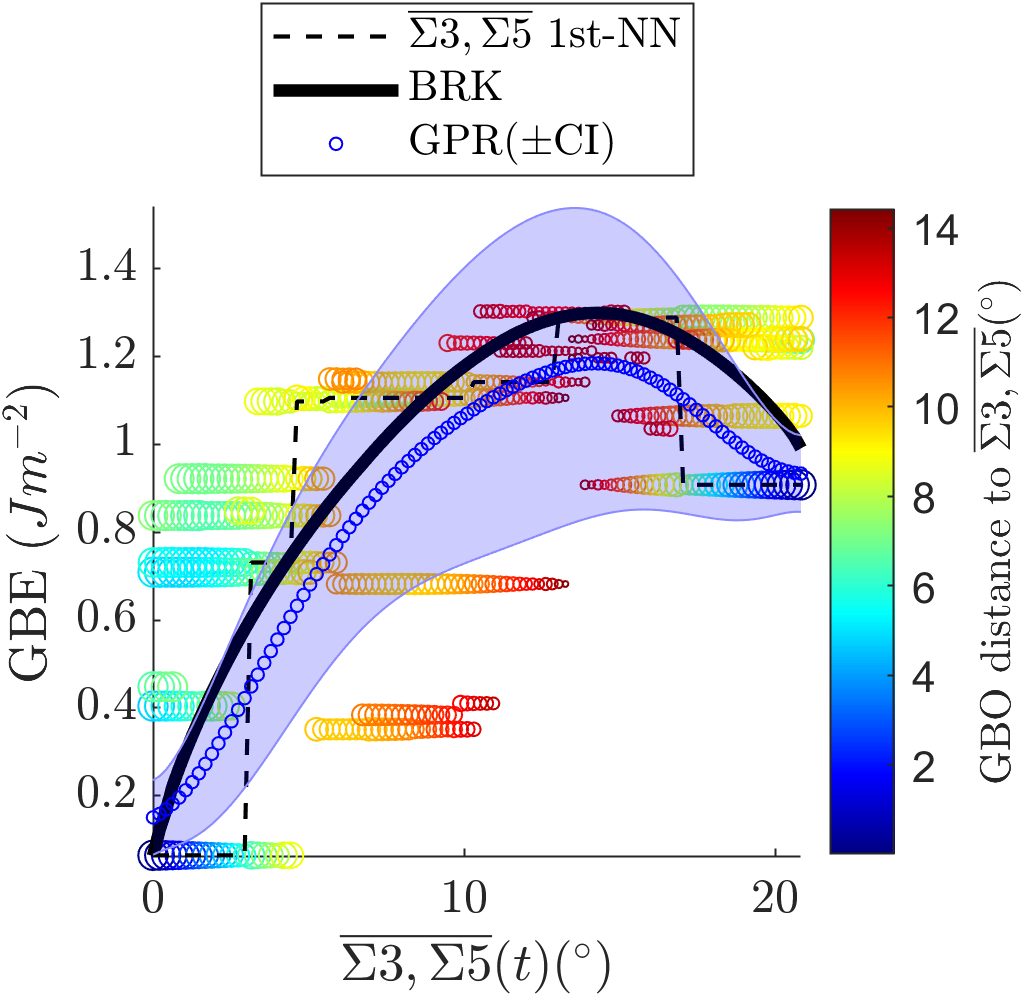
\includegraphics[width=\textwidth]{figures/tunnel-3-5-olmsted.png}
			\caption{}
			\label{fig:tunnel-3-5-olmsted}
		\end{subfigure}
% 		\hfill
		\begin{subfigure}[b]{0.4\textwidth}
			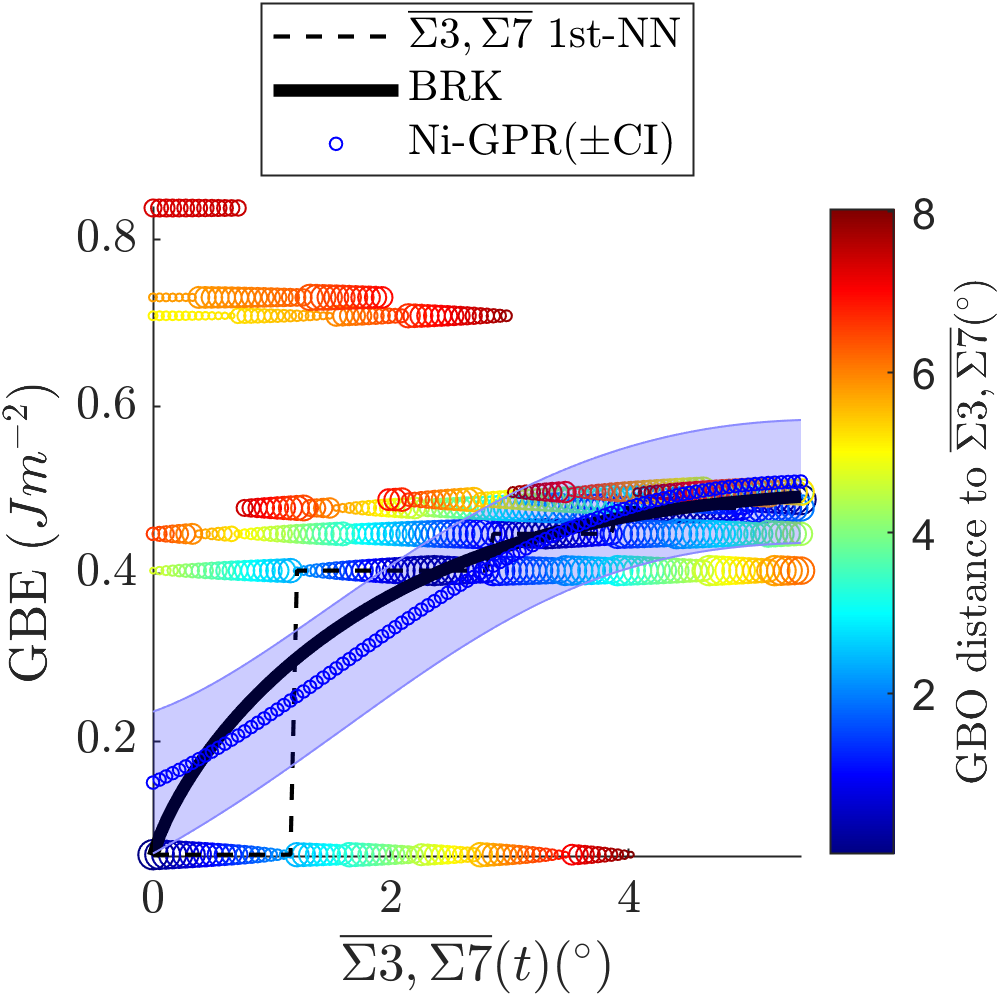
\includegraphics[width=\textwidth]{figures/tunnel-3-7-olmsted.png}
			\caption{}
			\label{fig:tunnel-3-7-olmsted}
		\end{subfigure}
		
		\begin{subfigure}[b]{0.4\textwidth}
			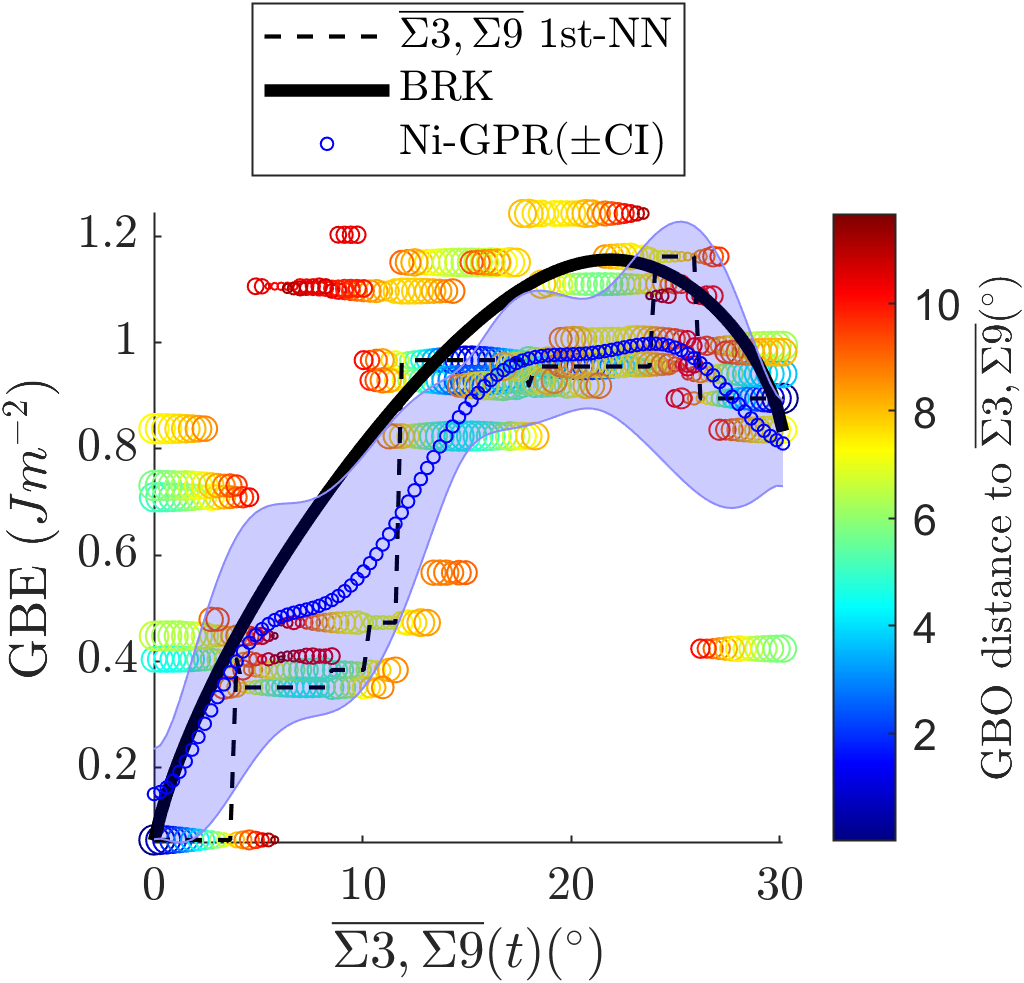
\includegraphics[width=\textwidth]{figures/tunnel-3-9-olmsted.png}
			\caption{}
			\label{fig:tunnel-3-9-olmsted}
		\end{subfigure}
% 		\hfill
		\begin{subfigure}[b]{0.4\textwidth}
			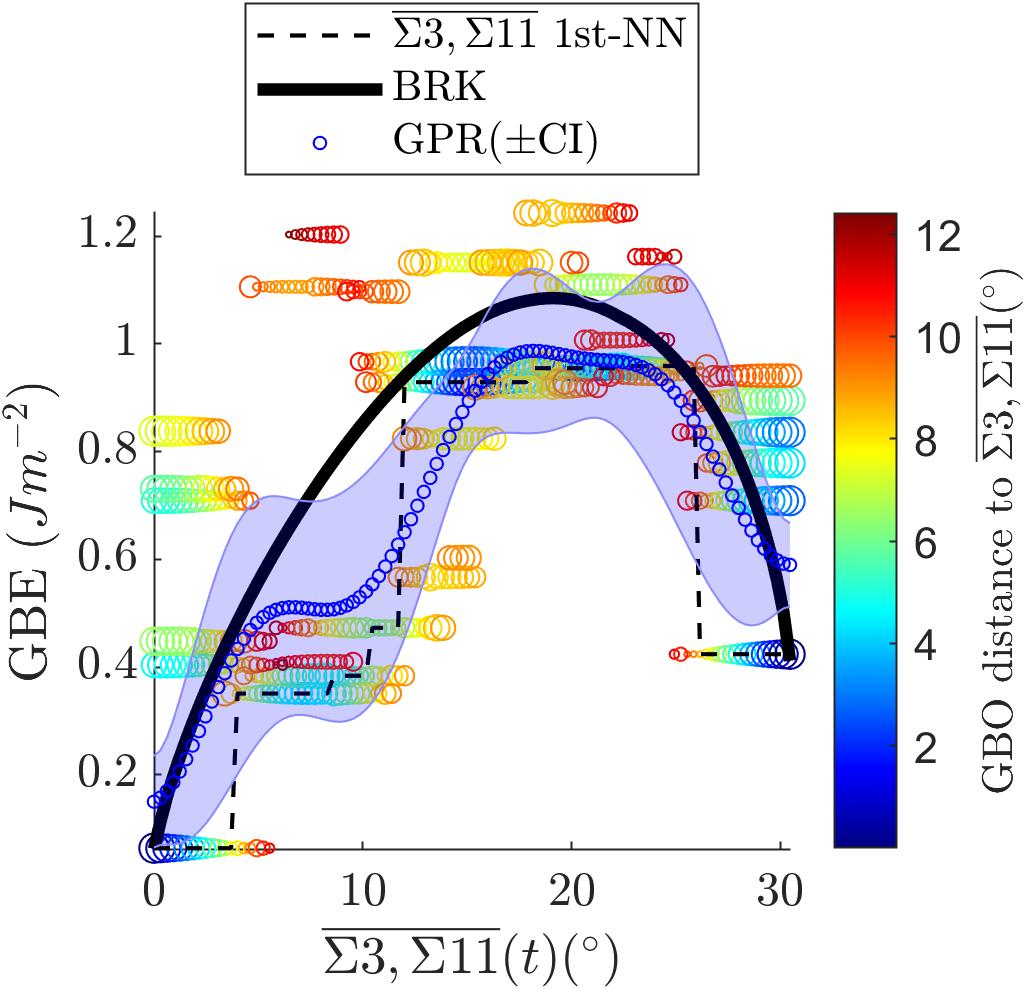
\includegraphics[width=\textwidth]{figures/tunnel-3-11-olmsted.png}
			\caption{}
			\label{fig:tunnel-3-11-olmsted}
		\end{subfigure}
		\caption{"Tunnel" plots of \glspl{gbe} along geodesic paths in a \gls{vfz} between the $\Sigma3$ \gls{ct} boundary and minimum \gls{gbe} (\subref*{fig:tunnel-3-5-olmsted}) $\Sigma5$, (\subref*{fig:tunnel-3-7-olmsted}) $\Sigma7$, (\subref*{fig:tunnel-3-9-olmsted}) $\Sigma9$, and (\subref*{fig:tunnel-3-11-olmsted}) $\Sigma11$ \glspl{gb} within the Ni \citet{olmstedSurveyComputedGrain2009a} dataset. \Gls{gbe} values are plotted for the \gls{brk} and \gls{gpr} models which both used \citet{olmstedSurveyComputedGrain2009a} as \inpt{} data. 95\% confidence intervals are plotted for the \gls{gpr} model. A "tunnel" plot is formed by calculating up to the 6th \glspl{nn} of the \inpt{} data relative to the geodesic path formed between two \glspl{gb}. The distances of the \glspl{nn} relative to the arc are used to both color and size the markers on the plot; \glspl{nn} which are closer to the arc are large, blue circles, whereas \glspl{nn} which are further from arc are small, red circles. Additionally, the 1st \gls{nn} path is plotted as a dashed line.}
		\label{fig:sigma-tunnels-olmsted}
	\end{figure*}
	
	\begin{figure*}[!htb]
		\centering
		\begin{subfigure}[b]{0.4\textwidth}
			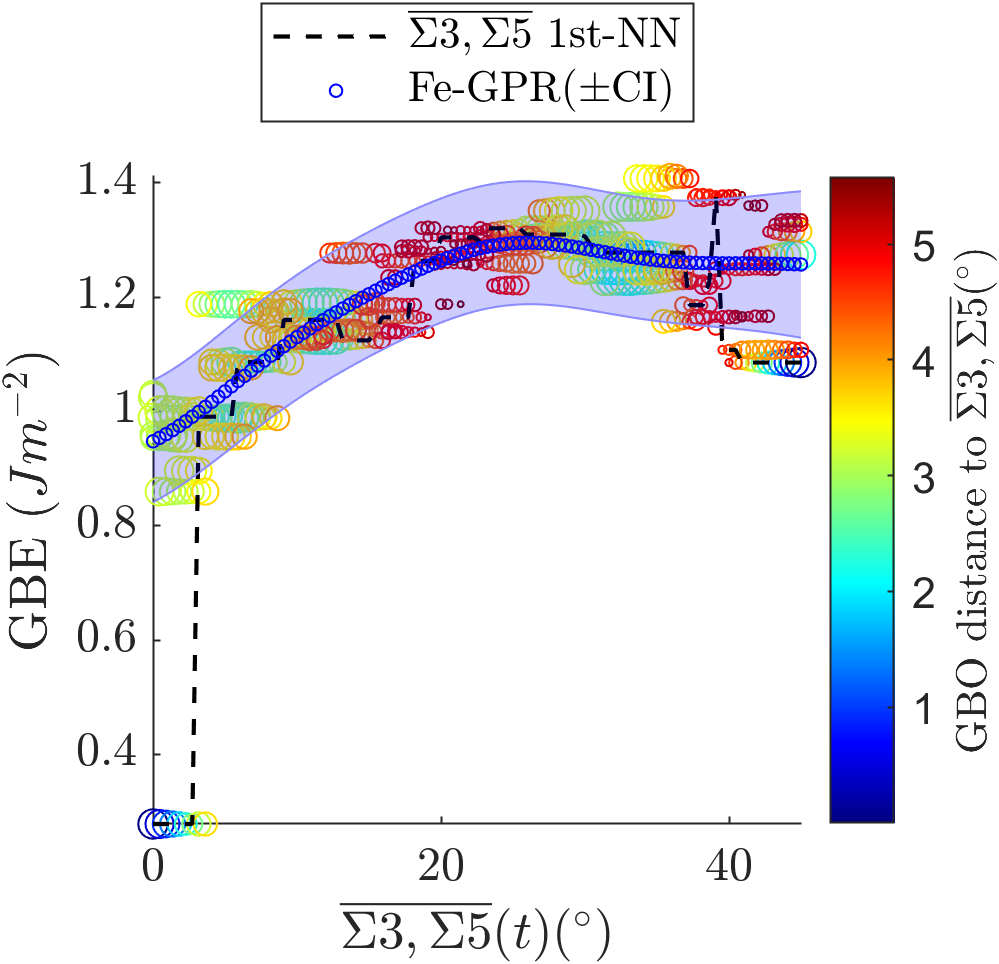
\includegraphics[width=\textwidth]{figures/tunnel-3-5-kim.png}
			\caption{}
			\label{fig:tunnel-3-5-kim}
		\end{subfigure}
% 		\hfill
		\begin{subfigure}[b]{0.4\textwidth}
			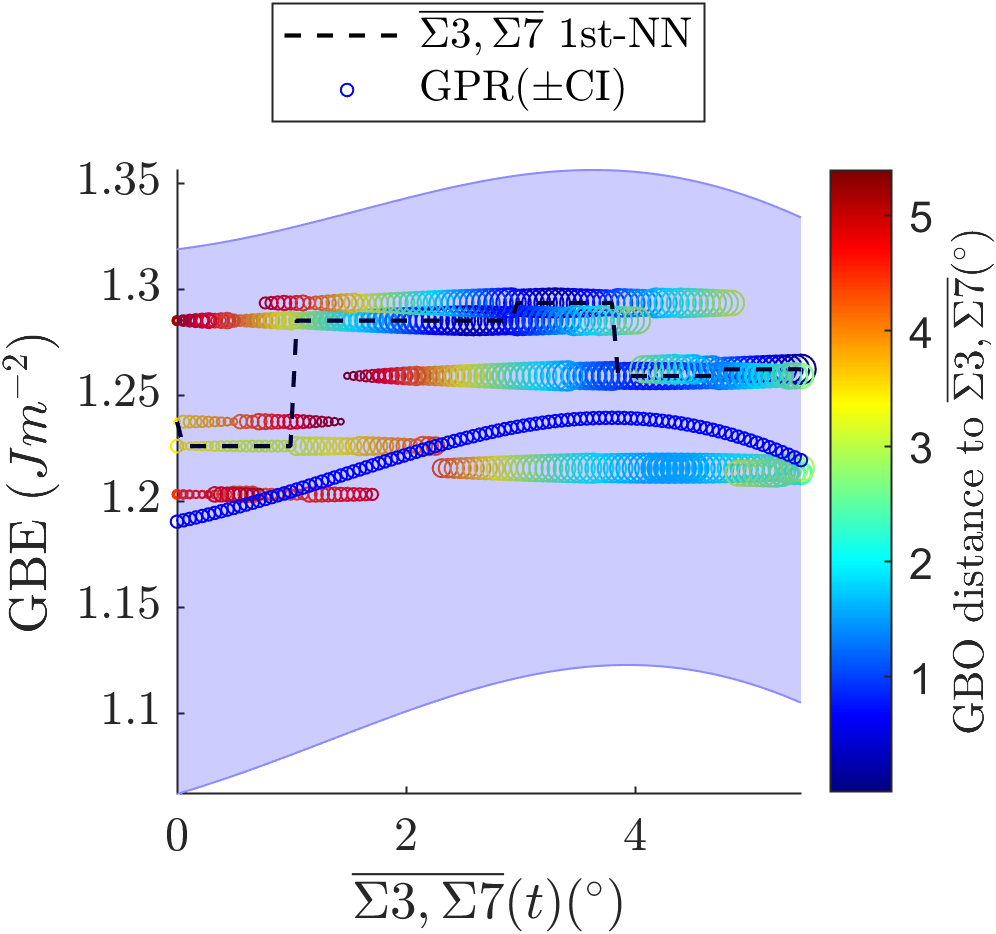
\includegraphics[width=\textwidth]{figures/tunnel-3-7-kim.png}
			\caption{}
			\label{fig:tunnel-3-7-kim}
		\end{subfigure}
		
		\begin{subfigure}[b]{0.4\textwidth}
			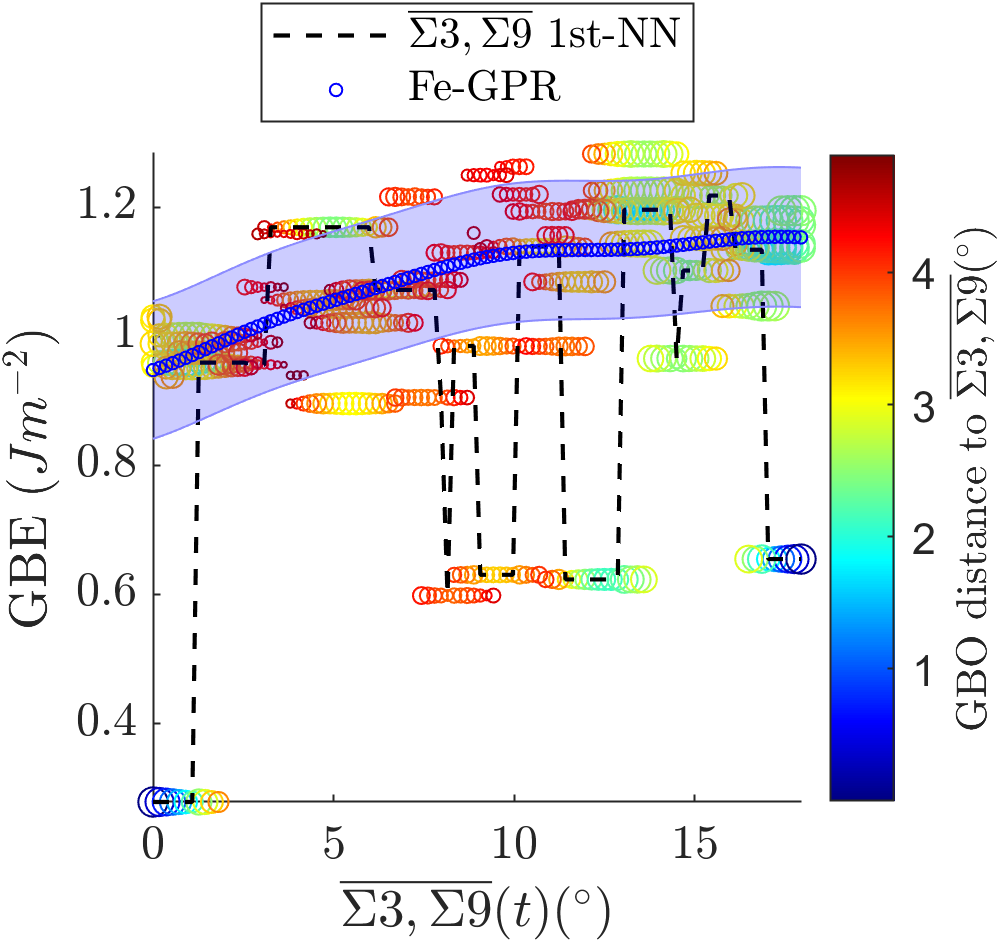
\includegraphics[width=\textwidth]{figures/tunnel-3-9-kim.png}
			\caption{}
			\label{fig:tunnel-3-9-kim}
		\end{subfigure}
% 		\hfill
		\begin{subfigure}[b]{0.4\textwidth}
			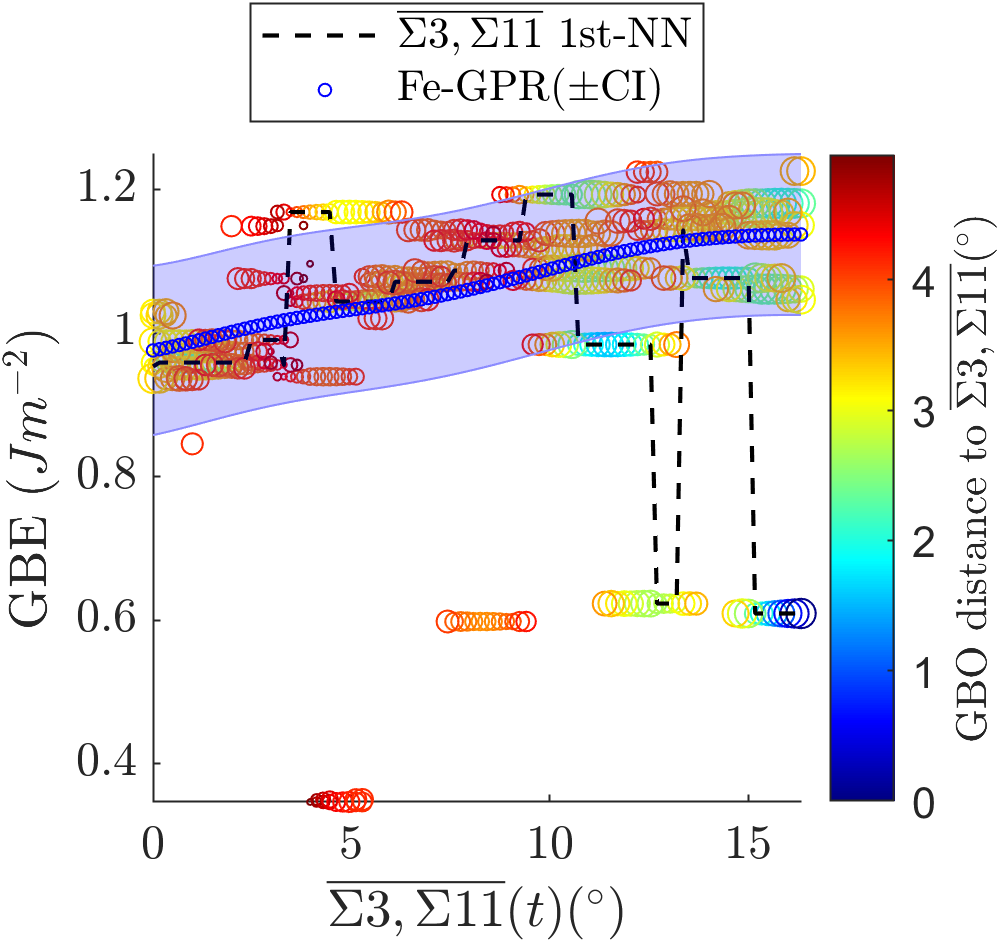
\includegraphics[width=\textwidth]{figures/tunnel-3-11-kim.png}
			\caption{}
			\label{fig:tunnel-3-11-kim}
		\end{subfigure}
		\caption{\Glspl{gbe} along geodesic paths in a \gls{vfz} between the minimum \gls{gbe} $\Sigma3$  and minimum \gls{gbe} (\subref*{fig:tunnel-3-5-kim}) $\Sigma5$, (\subref*{fig:tunnel-3-7-kim}) $\Sigma7$, (\subref*{fig:tunnel-3-9-kim}) $\Sigma9$, and (\subref*{fig:tunnel-3-11-kim}) $\Sigma11$ \glspl{gb} for the Fe \citet{kimPhasefieldModeling3D2014} dataset. A \gls{gpr} model trained on all \num{58604} Fe \citet{kimPhasefieldModeling3D2014} simulation datapoints was used. 95\% confidence intervals are plotted for the \gls{gpr} model. A "tunnel" plot is formed by calculating up to the 6th \glspl{nn} of the \inpt{} data relative to the geodesic path formed between two \glspl{gb}, similar to traveling through a 1D tunnel while also looking at nearby points in the region close to the line in all directions. The distances of the \glspl{nn} relative to the arc are used to both color and size the markers on the plot; \glspl{nn} which are closer to the arc are large, blue circles, whereas \glspl{nn} which are further from arc are small, red circles. Additionally, the 1st \gls{nn} path is plotted as a dashed line. }
		\label{fig:sigma-tunnels-kim}
	\end{figure*}
	
% 	 \subsection{\glsentrytitlecase{5dof}{short} Paths} \label{sec:discuss:path}
     We note that while the \gls{gbe} path is direct with respect to crystallographic distances, the actual rotation of a grain is not a barrier-free transformation and requires energy to induce the crystallographic change [REF]. Thus, when grain rotation and other non-spontaneous atomic transitions are involved, the true energy path can be thought of as a signal of local energy barriers associated with atomic movement superimposed on the \gls{5dof} paths shown.
     
     From another perspective, any transformation will depend on both the driving force and the activation energy. For example, near the transformation temperature, nucleation is slow because the driving force is small despite having fast diffusion. Likewise, at large undercoolings nucleation will be slow, but this time due to sluggish diffusion despite a large driving force. The \gls{gb} energy landscape tells us about the driving force for such a \gls{gb} crystallographic transformation, but it does not describe the activation energies of the atomic processes by which that transformation is achieved. Both pieces of information are necessary to predict whether and how fast a given crystallographic transformation might occur.

     For the \gls{gpr} model trained on the Ni \citet{olmstedSurveyComputedGrain2009a} dataset, we observe that the path from $\Sigma7$ to $\Sigma3$ is strictly downhill in energy in \cref{fig:tunnel-3-7-olmsted} while the geodesic paths between $\Sigma3$ and $\Sigma5$, $\Sigma9$, $\Sigma11$ are separated by energy barriers (\cref{fig:tunnel-3-5-olmsted,fig:tunnel-3-9-olmsted,fig:tunnel-3-11-olmsted}). This indicates that for grain growth systems governed by \gls{gbe}, it is possible that a $\Sigma7$ \gls{gb} may transform into a $\Sigma3$ \gls{gb}, if the mechanisms required to traverse this trajectory in the \gls{gb} energy landscape are available (e.g. if both grain rotation and plane reorientation are possible, such as during high-temperature plastic deformation, recrystallization, or in nanocrystalline materials). In contrast, for a $\Sigma5$, $\Sigma9$, or $\Sigma11$ \glspl{gb} to transform into $\Sigma3$ \glspl{ct}, either an energy barrier must be overcome, or a different (perhaps more circuitous) trajectory through the \gls{5dof} space must be taken.
     
     For the \gls{gpr} model trained on the Ni data (\cref{fig:sigma-tunnels-olmsted}), the substantial vertical spread of the 1st-6th \glspl{nn} (colored, variable-size circles) are consistent with the fact that many points have distances on the order of \num{8}$-$\SI{14}{\degree} relative to the geodesic path between the two \glspl{gb}. For perspective, these distances are greater than the global correlation length of \SI{7.4}{\degree} (\cref{sec:results:correlation:global}), for which a higher proportion of distant points from the models are also distant crystallographically (small red and yellow circles). In other words, these trajectories traverse regions of the \gls{vfz} that are sparsely populated with data.
     
     For the \gls{gpr} model trained on the Fe \citet{kimPhasefieldModeling3D2014} dataset, the 1st \gls{nn} path and the \gls{gpr} path have substantial qualitative deviation from each other for $\overline{\Sigma3,\Sigma9}$ and $\overline{\Sigma3,\Sigma11}$ paths. While the \gls{gpr} model suggests that $\overline{\Sigma3,\Sigma11}$ are connected, the 1st \gls{nn} path suggests that there are local minima that are overestimated. Likewise, the 1st-6th \glspl{nn} (colored, variable-size circles) for $\overline{\Sigma3,\Sigma5}$ and $\overline{\Sigma3,\Sigma7}$ follow the general trend of the models. We observe that all \glspl{nn} distances up to the 6th \gls{nn} are less than $\sim$\SI{6}{\degree} from the paths of interest; this in turn is less than the global correlation length of \SI{8.3}{\degree} from \cref{sec:results:correlation:global} which indicates that local regions of influence along these paths in the Fe dataset are densely populated.
     
     By contrast, some \glspl{nn} have vastly different energies compared with the \gls{gpr} model. This is because the noise of the simulated \glspl{gbe} (\cref{sec:results:lit:error}) precludes the \gls{gpr} model from simultaneously resolving sharp transitions and maintaining smooth behavior elsewhere. This is one of the drawbacks of using a noisy dataset in a diverse space (some regions with sharp cusps, others with shallow hills and valleys) with a global smoothness (i.e. correlation) length.
	 %
	
	\subsection{Potential for Numerical Derivatives}
	\label{sec:results:deriv}
	
	 \Gls{gb} path visualizations in the \gls{vfz} framework suggest the ability to estimate numerical derivatives or gradients of \gls{gb} properties without being restricted to a \gls{gb} subspace (e.g. \gls{mfz} or \gls{bpfz}) which can be a useful mathematical construct for the \gls{gb} community. For example, steepest descent paths can be estimated and used in grain growth simulations.
	
	Because distance overestimations exist in the standard \gls{vfz} framework, use of ensembled \gls{vfzgbo} interpolation or data augmentation may be necessary to mitigate discontinuity artifacts when crossing the exterior of a \gls{vfz} as discussed in \cref{sec:methods:framework}. Alternatively, the "excess" points in a gridded sampling can act as a type of data augmentation and help to address this issue. We plan to explore these topics in future work. \Cref{sec:supp:grid} contains further discussion of a gridded sampling approach.
	 
	\section{Conclusion} \label{sec:conclusion}
	We applied the \gls{vfz} framework to learning more about the nature of a \gls{5dof} \gls{fz}.

	The increase of distance computation throughput and the development of a \gls{5dof} \gls{vfz} with continuous coordinates enabled us to explore the nature of a \gls{5dof} \gls{fz}. We found that symmetrized \gls{nn} distance distributions are Gaussian and plotted these as a function of set size. Additionally, we found the \gls{gbe} correlations to be Gaussian. We determined the maximum principal component of a particular $O_h$ \gls{vfz} to be \dimOne{}.
	
	Other point groups (in particular those which are noncentrosymmetric) may give rise to differently shaped/larger \glspl{vfz} and for which the Euclidean approximation may need to be removed. It will be interesting to see the \gls{vfz} framework applied for other distance metrics (see \citet{morawiecDistancesGrainInterfaces2019} for a comprehensive summary of metrics).

	The interpolation errors for a Fe simulation dataset are on par with the intrinsic uncertainty of the dataset itself (\cref{sec:supp:kim-interp:quality}). Analysis of the \gls{gpr} fitting results indicates that the Ni and Fe simulation datasets have correlation lengths of \SIlist{8.3;7.4}{\degree}, respectively, but that when the Ni dataset is constrained to have low noise, the numerical correlation length drops to $\sim$\SI{1.9}{\degree}.
	%DISCUSS pairwise correlations & BRANDON'S CRITERIA, 2-4 sentences
	%
	Plotting of geodesic paths between low-Sigma \glspl{gb} of interest reveal that a $\Sigma$7 cusp has a monotonically decreasing path towards the \gls{ct} $\Sigma3$ cusp, whereas a $\Sigma5$, $\Sigma9$, and $\Sigma11$ cusps do not necessarily share this same type of monotonically decreasing path within a \gls{vfz}. We demonstrated that two cusps can be connected in \gls{5dof} space.
	
	In addition to its previous implementation for \gls{gb} property interpolation \cite{bairdFiveDegreeofFreedomPropertyUnderReview}, we anticipate the \gls{vfz} framework will continue to reveal important aspects of a \gls{5dof} \gls{fz} and inform us about material behavior especially with respect to grain growth and other large scale time-dependent or iterative processes.

	\section*{Acknowledgement}
	\label{sec:acknowledgement}
	
	The authors thank Ian Chesser, Toby Francis, Victoria Baird, Brandon Snow, and José Niño for useful discussions. This work was supported by the National Science Foundation under Grant No. 1610077. This work was supported in part through computational resources provided by Brigham Young University's Office of Research Computing.
	\section*{CRediT Statement}
	\textbf{Sterling Baird}: Conceptualization, Methodology, Software, Validation, Formal analysis, Investigation, Data Curation, Writing - Original Draft, Writing - Review \& Editing, Visualization. \textbf{Oliver Johnson}: Supervision, Project administration, Funding acquisition, Conceptualization, Writing - Review \& Editing. \textbf{David Fullwood}: Writing - Review \& Editing. \textbf{Eric Homer}: Funding acquisition, Writing - Review \& Editing

	
	% \appendix
\label{sec:app}
\section{Detailed Barycentric Interpolation Methods}
\setcounter{figure}{0}
\subsection{Triangulating a \glsentrytitlecase{vfz}{long} Mesh}
\label{app:bary-tri}

% Briefly (but clearly and explicitly) explain the steps of generating the cubochorically sampled GBs, converting them to octonions and then mapping all of them into the vfz. Then explain how you do the triangulation. This will require a few figures to show the process in 3D (i.e. generating a triangulation of a point cloud on a region of the surface of the 2-sphere).

% After random \glspl{vfzo} are obtained (\cref{sec:methods:rand}), % ...

In order to reduce the computational complexity of triangulating a high-dimensional mesh \cite{barberQuickhullAlgorithmConvex1996}, some simplifications are made. The degenerate dimension obtained from analytically minimizing $U(1)$ symmetry \cite{francisGeodesicOctonionMetric2019} is first removed via a rigid (i.e. distance- and angle-preserving) \gls{svd} transformation,
%to enable use of MATLAB's quickhull \cite{barberQuickhullAlgorithmConvex1996} implementations such as \texttt{delaunayn} and \texttt{convhulln}. Removal of the degenerate dimension is done via a rigid \gls{svd} transformation,
analogous to a Cartesian rotation and translation
%Thus, a set of octonions originally represented by 8D Cartesian coordinates are collapsed to a 7D Cartesian representation while preserving both distances and angles among the points
As a 3D Cartesian to 2D Cartesian analogue of this 8D Cartesian to 7D Cartesian transformation, we take a set . Next, this 7D Cartesian representation is projected onto a hyperplane tangent to the mean of the input points\footnote{This is \textit{not} a rigid transformation; however, it is sufficiently close to produce a high-quality triangulation in a \gls{vfz}.} (\cref{fig:bary-delaunay}b). The 7D Cartesian \glspl{gbo} undergo another rigid \gls{svd} transformation to 6D Cartesian (see 3D to 2D analogue in \cref{fig:bary-delaunay}c) for which a triangulation is computed via the quickhull algorithm \cite{barberQuickhullAlgorithmConvex1996} (see MATLAB function \texttt{delaunayn}).

\begin{figure}
    \centering
    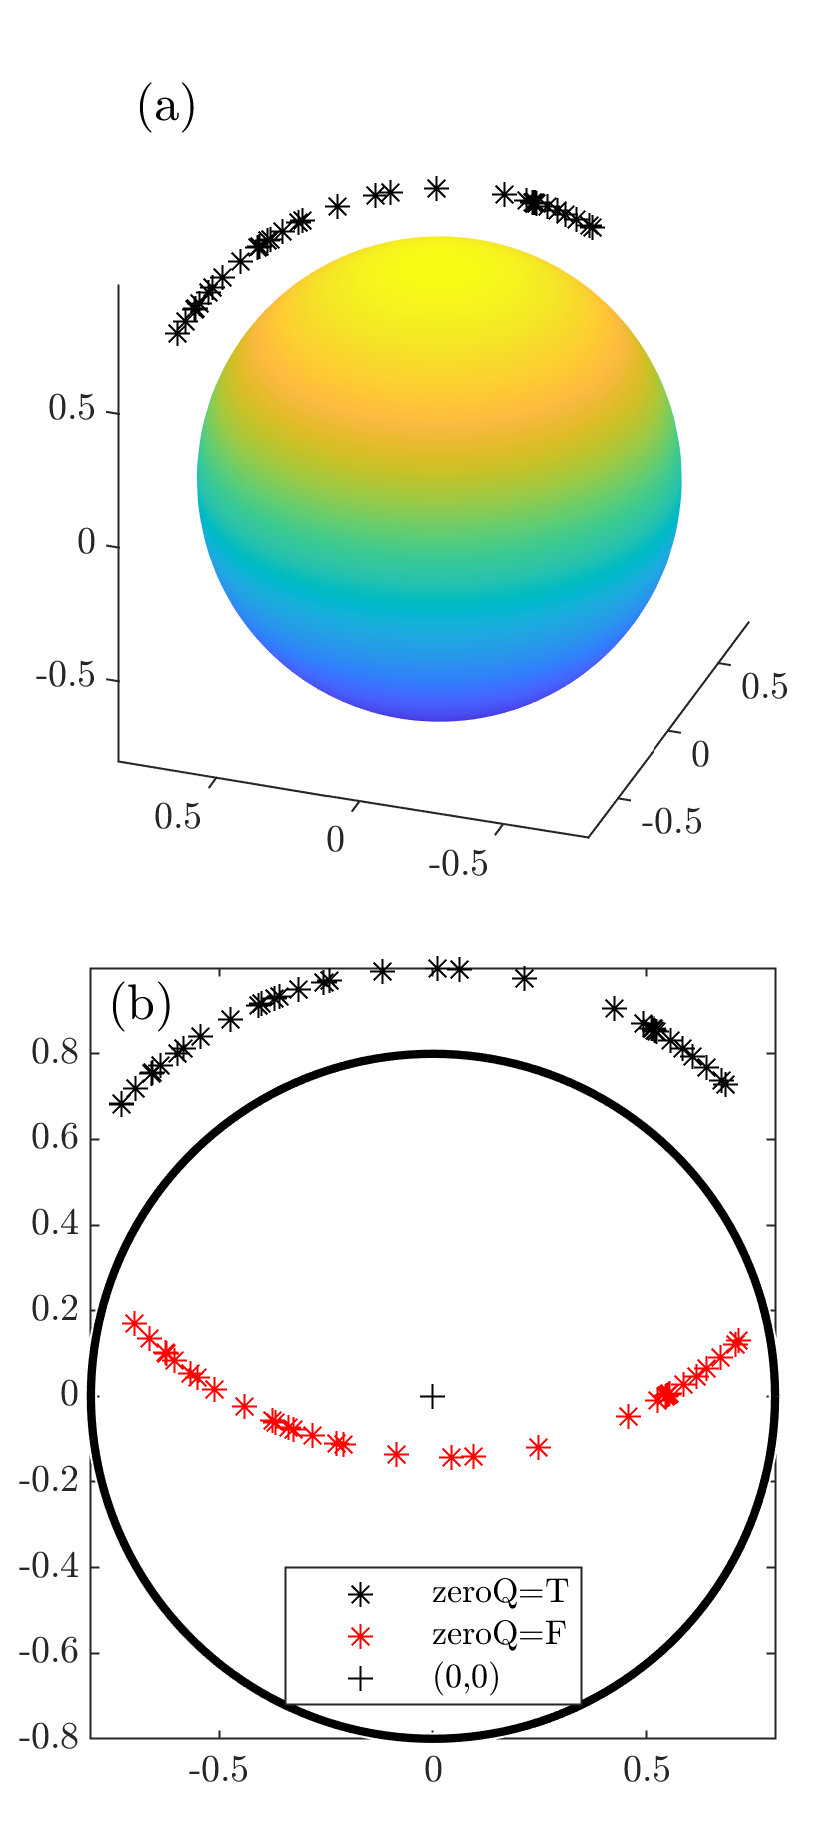
\includegraphics[scale=1]{bary-remove-deg.png}
    \caption{3D Cartesian to 2D Cartesian analogue of 8D Cartesian to 7D Cartesian degeneracy removal used in barycentric interpolation approach. Starting spherical arc points on surface of 2-sphere (a) and degenerate dimension removed via \acrlong{svd} transformation to 2D Cartesian (b) with either the origin (black plus) preserved (black asterisks, \texttt{zeroQ=T}) or ignored (red asterisks, \texttt{zeroQ=F}). The sphere (a) and circle (b) each have a radius of 0.8 and are used as a visualization aid only.}
    \label{fig:bary-remove-deg}
\end{figure}

Using a separate rigid \gls{svd} transformation from the triangulation, the original mesh and prediction \glspl{gbo} are simultaneously transformed from 8D Cartesian to 7D Cartesian. Because our \gls{svd} approach is rigid, the triangulation is then superimposed onto the newly transformed input points resulting in a 7D Cartesian \gls{vfz}.

\begin{figure}
    \centering
    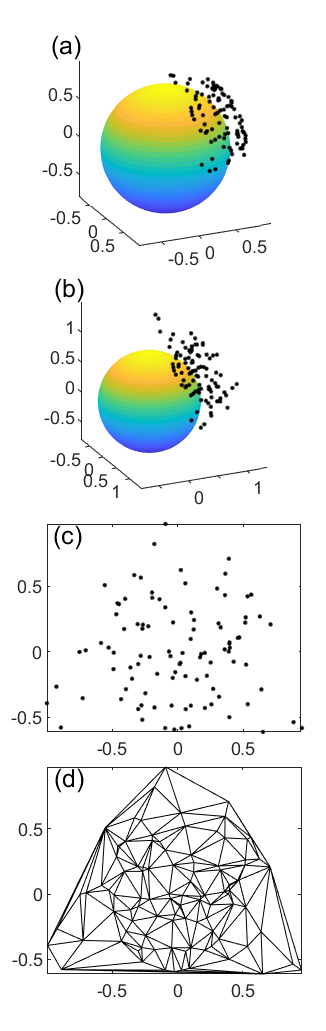
\includegraphics[scale=1]{bary-delaunay.png}
    \caption{3D Cartesian to 2D Cartesian analogue of 7D Cartesian to 6D Cartesian mesh triangulation used in barycentric interpolation approach. Input points linearly projected projected onto hyperplane tangent to mean of starting points (a), degenerate dimension removed via rigid \gls{svd} transformation to 2D Cartesian and Delaunay triangulation calculated (b), and Delaunay triangulation superimposed onto normalized input points. The spheres in (a) and (c) have a radius of 0.8 and is used for visualization only.}
    \label{fig:bary-delaunay}
\end{figure}

% In order to reduce the computationally complexity of computing barycentric coordinates in a high-dimensional space \cite{barberQuickhullAlgorithmConvex1996}, a single degenerate dimension (originally introduced by analytically minimizing $U(1)$ symmetry) is removed to enable use of MATLAB's quickhull \cite{barberQuickhullAlgorithmConvex1996} implementations such as \texttt{delaunayn} and \texttt{convhulln}. Removal of the degenerate dimension is done via a rigid \gls{svd} transformation, analogous to a Cartesian rotation and translation. Thus, a set of octonions originally represented by 8D Cartesian coordinates are collapsed to a 7D Cartesian representation while preserving both distances and angles among the points (see 3D to 2D analogue in \cref{fig:bary-remove-deg}). To further reduce the "curse of dimensionality" in computing the triangulation, a 7D Cartesian representation of the octonions constrained to lie on the surface of the 6-sphere are first projected onto a hyperplane tangent to the mean of the input points and then rotated/translated again via \gls{svd} to produce a 6D Cartesian representation (see 3D to 2D analogue in Figure \cref{fig:bary-delaunay}). This 6D representation is used to compute a triangulation via the built-in MATLAB routine \texttt{delaunayn} based on the quickhull algorithm \cite{barberQuickhullAlgorithmConvex1996}, giving facet vertices for the 7D Cartesian hypersphere.

\subsection{Intersections in a \glsentrytitlecase{vfz}{long} Mesh}
\label{app:bary-int}
An intersection is calculated by linearly projecting a prediction point onto the hyperplane defined by a mesh facet's vertices (\cref{fig:bary-interp}, computing barycentric coordinates within the facet, and testing for positivity \cite{langerSphericalBarycentricCoordinates2006}, and repeating this process until an intersection is found or a stop condition is reached (see \texttt{nnMax} below). If the prediction point is contained within the simplex, all of the barycentric weights (i.e. coordinates) are positive. If it outside the simplex, this constraint is violated. Due to the large number of facets per point of a high-dimensional
%simplex-based
triangulation
%and for computational speed,
prediction point intersections are calculated by considering facets connected to up to some number of mesh \glspl{nn} (\texttt{nnMax}) (in this work, \texttt{nnMax = 10}). For prediction points where no intersecting facet is found
%in these connected facets due to high-aspect ratio facets or prediction point falling outside the mesh within a given tolerance,
a \gls{nn} approach is used (\cref{sec:methods:interp:nn}), which represent average non-intersection rates of \SI{0.1207 \pm 1.02}{\percent} and \SI{0.68 \pm 0.11}{\percent} for input meshes of \num{388} and \num{50000}, respectively, for \num{10000} query points out of \num{10} trials.

\subsection{Interpolation via Barycentric Coordinates}
\label{app:bary-interp}

Once barycentric coordinates are computed for a prediction point within the input mesh, the interpolated value is found by taking the dot product of the barycentric coordinates and the properties of the corresponding vertices of the intersecting facet via
\begin{equation}
\label{eq:bary-interp}
v=\underset{i=1}{\overset{N}{\sum }}\lambda _i v_i
\end{equation}
where $\lambda$, $v$, $v_i$ and $N$, are the barycentric coordinates, interpolated property, property of the $i$th vertex of the intersecting facet, and number of vertices in a given facet ($N = 7$ for the degeneracy-free 6-sphere). A 2-sphere example is provided in \cref{fig:bary-interp}.

\begin{figure}
    \centering
    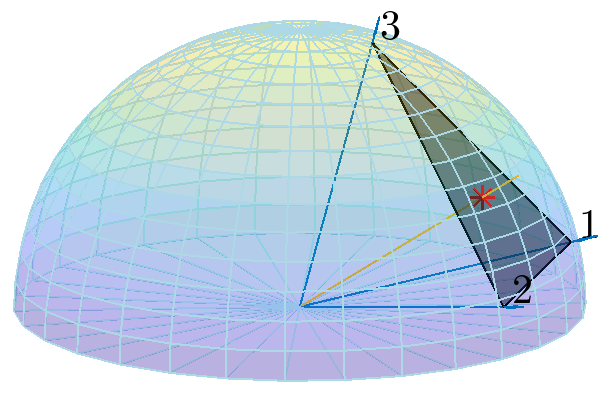
\includegraphics[scale=1]{bary-interp.png}
    \caption{A ray (red line) on the 2-sphere is linearly projected onto the hyperplane of a mesh facet (transparent black), shown as a red asterisk. The barycentric coordinates are computed as $\lambda_{i \in [1,3]} = \frac{1}{3}$. Because all barycentric coordinates are positive, it is determined that the projected point is an intersection with the mesh. Given vertex values of \num{8.183}, \num{3.446}, and \num{3.188} for vertices 1, 2, and 3, respectively, the interpolated value is calculated as \num{4.94} via \cref{eq:bary-interp}.}
    \label{fig:bary-interp}
\end{figure}
	
	% \appendix
	\begin{appendices}
		
		\crefalias{section}{appsec}
		\crefalias{subsection}{appsec}
		\crefalias{subsubsection}{appsec}
		
	\end{appendices}
	
	% \newpage
	\printglossaries
	% \printabbreviations
	%need to manually clear cached files & logs in overleaf to get new abbreviations to appear, maybe?
	
	% \newpage
	\bibliographystyle{elsarticle-num-names}
	\bibliography{5dof-gb-energy.bib}
	
	% \begin{enumerate}
    \item First mesh-based property interpolation scheme that incorporates all five macroscopic crystallographic degrees of freedom.
    \item Past work predicting grain boundary energy
    \begin{enumerate}
        \item \gls{brk} function \cite{Bulatov2014GrainMetals}
        \item Rohrer \gls{gbed} based on binning in nickel \cite{Li2009RelativeNickel}, yttria \cite{Dillon2009CharacterizationFIB}, and copper \cite{Randle2008Five-parameterCopper}. Also \cite{Rohrer2010DerivingData}
        \item other five-parameter articles: titanium \cite{Farabi2018Five-parameterTitanium}, BCC materials \cite{Ratanaphan2015GrainMetals}.
        \item a non-discretizing \gls{knn} approach to determine GB energy \cite{Shen2019DeterminingSpace}.
        \item Neural network predictions \cite{EcheverriRestrepo2014UsingEnergies}
        \item grain boundary octonion theory \cite{Francis2019ABoundaries,Chesser2020LearningProperties}
         \begin{enumerate}
             \item Smooth interpolation between two arbitrary grain boundaries (oSLERP) \cite{Francis2019ABoundaries}
             \item inverse distance weighting approach \cite{Chesser2020LearningProperties}
         \end{enumerate}
    \end{enumerate}
    
    \item extension of octonion representation using barycentric coordinates
    \begin{enumerate}
        \item barycentric coordinates commonly used for interpolation within a simplex or other convex polygon.
        \begin{enumerate}
            \item basic equations (positivity, partition of unity, linear precision) \cite{Langer2006SphericalCoordinates}
        \end{enumerate}
        \item spherical barycentric coordinates that preserve linear precision \cite{Langer2006SphericalCoordinates}, which is important for interpolation, or preserve partition of unity \cite{Lei2020ASystems}, which is better for even subdivision of spherical surfaces.
        \item we incorporate linear precision preserving barycentric coordinates with an octonion representation of GBs to do property interpolation.
    \end{enumerate}
    \item application of this octonion framework using Gaussian process regression
    \begin{enumerate}
        \item Gaussian process regression is a machine learning technique geared towards predicting data (along with prediction intervals and standard deviations of the predictions) for arbitrary regions using a set of input data consisting of predictors and responses.
        \item By supplying a closed octonion mesh, we compute covariance matrices efficiently (i.e. arbitrary distance calculations are very quick), which is important for a Gaussian process regression.
    \end{enumerate}
\end{enumerate}

\section{Results and Discussion} \label{sec:resultsDiscussion}
\begin{enumerate}
    \item parity plots
    \begin{enumerate}
        \item 388 and 50,000 mesh points
        \item tile1 - spherical barycentric interpolation
        \item tile2 - planar barycentric interpolation
        \item tile3 - \gls{gpr}
        \item tile4 - pure \gls{nn} interpolation
    \end{enumerate}
    \begin{figure}
        \centering
        \includegraphics{}
        \caption{parity plots for 388 (red) and 50,000 (black) octonions formed via pairs of random cubochorically sampled quaternion and spherically sampled boundary plane normals. Property values sampled via \acrlong{brk} function and interpolation via barycentric (a), pure \acrlong{nn} (b), and \acrlong{gpr} (c).}
        \label{fig:brk-parity1}
    \end{figure}
    \begin{figure}
        \centering
        \includegraphics{}
        \caption{parity plots for 388 Olmsted \acrfullpl{gb} (red) and 50,000 Kim \acrshortpl{gb} (black) with property values sampled via \acrlong{brk} function and interpolation via barycentric (a), pure \acrlong{nn} (b), and \acrlong{gpr} (c).}
        \label{fig:brk-parity2}
    \end{figure}
    \item \Gls{rmse} vs. number mesh points for barycentric interpolation (black), \gls{gpr}, and pure \gls{nn} interpolation (red). Range from 1e2 to 1e5 mesh points
    \begin{figure}
        \centering
        \includegraphics{}
        \caption{\acrlong{rmse} vs. number of mesh points for spherical barycentric interpolation (black), planar barycentric interpolation, spherical \acrlong{gpr} (red), planar \gls{gpr}, pure \acrlong{nn} interpolation (orange), and average model with standard deviations from 10 random samples.}
        \label{fig:brk-rmse}
    \end{figure}
    \item histograms of \gls{nn} and next \gls{nn} distances (arc length) for mesh
    \begin{figure}
        \centering
        \includegraphics{}
        \caption{histograms of \acrfull{nn} (red) and next \acrlong{nn} (black) arc lengths for meshes of 388 (a), 10,000 (b), and 50,000 (c) octonions formed via pairs of random, cubochorically sampled quaternions.}
        \label{fig:nndist}
    \end{figure}
    \item timing and efficiency
    \begin{enumerate}
        \item fitrgp produces lower error in less time than barycentric interpolation even when using sparse approximation methods.
        \item barycentric interpolation is very fast once the triangulation is computed (i.e. still fast even if responses change, but needs to be recomputed if input data, i.e. predictors, change)
        \item fitrgp is fast and has lower error compared to barycentric interpolation; however, the entire process has to be rerun (in current implementation) if the responses or the predictors change.
    \end{enumerate}
    \item comparison with Chesser \cite{Chesser2020LearningProperties} (few points, Ni data, both high- and low-symmetry sets). Use 388 Ni bicrystals instead of \gls{brk} function. Barycentric and \gls{gpr}
    \begin{enumerate}
        \item table
        \begin{table}[]
            \centering
            \begin{tabular}{c c c c}
                \hline
                 Method & Minimizing Distance & \acrshort{rmse} & \acrshort{mae} \\
                 \hline
                 Barycentric & Euclidean Norm & & \\
                 \acrshort{nn} & Euclidean Norm & & \\
                 \acrshort{gpr} & Euclidean Norm & & \\
                 Pairwise-distance & Arc Length & &
            \end{tabular}
            \caption{Comparison of \acrfull{rmse} and \acrfull{mae} for closed-mesh barycentric interpolation, closed-mesh \acrfull{nn} interpolation, closed-mesh \acrfull{gpr}, and pairwise-distance inverse weighting for 388 Ni bicrystal simulations with 10-fold cross validation for each method.}
            \label{tab:chesser-comp}
        \end{table}
        \item parity plot
        \item \gls{5dof} visualizations
        \begin{figure}
            \centering
            \includegraphics{}
            \caption{\acrfull{gb} energy plotted in the $\Sigma{3}$, $\Sigma{5}$, $\Sigma{7}$, and $\Sigma{11}$ \acrlong{bp} spaces for closed-mesh spherical barycentric (a) and \acrlong{nn} (b) interpolation, closed-mesh \acrlong{gpr} (c), and pairwise-distance inverse weighting using 388 Ni bicrystal simulations.}
            \label{fig:chesser-5dof}
        \end{figure}
        \item 1DOF curves ([100] and [110] symmetric tilt boundaries ?)
    \end{enumerate}
    \item comparison with Restrepo \cite{EcheverriRestrepo2014UsingEnergies} (many points, Fe data, both high- and low-symmetry sets). Use simulated Fe data instead of \gls{brk} function. Barycentric and \gls{gpr}
    \begin{enumerate}
        \item table
        \begin{table}[]
            \centering
            \begin{tabular}{c c c c}
                \hline
                 Method & Minimizing Distance & \acrshort{rmse} & \acrshort{mae} \\
                 \hline
                 Barycentric & Euclidean Norm & & \\
                 \acrshort{nn} & Euclidean Norm & & \\
                 \acrshort{gpr} & Euclidean Norm & & \\
                 \acrshort{ann} & N/A & &
            \end{tabular}
            \caption{Comparison of \acrfull{rmse} and \acrfull{mae} for closed-mesh barycentric interpolation, closed-mesh \acrlong{gpr}, and a non-symmetry considering \acrfull{ann} using 50,000 Fe bicrystal simulations.}
            \label{tab:restrepo-comp}
        \end{table}
        \item parity plot
        \item \gls{5dof} visualizations
        \begin{figure}
            \centering
            \includegraphics{}
            \caption{\acrfull{gb} energy plotted in the $\Sigma{3}$, $\Sigma{5}$, $\Sigma{7}$, and $\Sigma{11}$ \acrlong{bp} spaces for closed-mesh spherical barycentric (a) and \acrlong{nn} (b) interpolation, closed-mesh \acrlong{gpr} (c), and a non-symmetry considering \acrlong{ann} (d) using 50,000 Fe bicrystal simulations.}
            \label{fig:restrepo-5dof}
        \end{figure}
        \item 1DOF curves ([100] and [110] symmetric tilt boundaries ?)
    \end{enumerate}
\end{enumerate}


\section{Methods} \label{sec:methods}

\begin{enumerate}
    \item barycentric interpolation
    \begin{enumerate}
        \item commonly used for interpolation within a simplex or other convex polygon.
        \begin{enumerate}
            \item basic equations (positivity, partition of unity, linear precision) \cite{Langer2006SphericalCoordinates}
        \end{enumerate}
        \item spherical barycentric coordinates that preserve linear precision \cite{Langer2006SphericalCoordinates}, which is important for interpolation, or preserve partition of unity \cite{Lei2020ASystems}, which is better for even subdivision of spherical surfaces.
    \end{enumerate}
    \item Gaussian process regression
    \begin{enumerate}
        \item MATLAB fitrgp
        \begin{enumerate}
            \item squared exponential covariance function
            \item bcd fit method (others are sd, fic etc.)
            \item constant basis function
            \item exact or bcd predict methods (also fic)
            \item quasi-newton optimizer
            \item optimize KernelScale and Sigma hyperparameters with bayesopt Optimizer
            \item ActiveSetMethod - entropy (others, log likelihood, sparse greedy approximation)
        \end{enumerate}
    \end{enumerate}
\item combining octonion representation with barycentric interpolation or Gaussian process regression
    \begin{enumerate}
        \item choosing a symmetrically equivalent representation based on minimum euclidean norm using a single reference octonion (i.e. kept constant)
        \begin{enumerate}
            \item contrast with traditional approach \cite{Francis2019ABoundaries}
            \begin{enumerate}
                \item traditional: allows either octonion to vary for efficiency; ours: one octonion held constant
                \item traditional: use arc length as minimizing metric; ours: use euclidean norm
                \item traditional: consider a subset of symmetrically equivalent GBOs; ours: consider all symmetrically equivalent GBOs
                \item traditional: always stay in 8D representation; ours: remove degenerate dimension (to 7D) for interpolation and employ projections (to 6D) for triangulation efficiency (for barycentric interpolation)
            \end{enumerate}
        \end{enumerate}
        \item triangulating a set of octonions using qhull (for barycentric interpolation)
        \item projections and rotations (projection to hyperplane, singular value decomposition)
        \item spherical barycentric coordinates \cite{Langer2006SphericalCoordinates}
        \begin{enumerate}
            \item equations
        \end{enumerate}
        \item barycentric interpolation
        \begin{enumerate}
            \item equations
            \item Determine intersecting facet using facets connected to \gls{nn}s and positivity constraint of planar barycentric coordinates
            \item intersecting facet vertices projected onto hyperplane tangent to hypersphere at datapoint
            \item containing facet and barycentric coordinates only need to be computed once for each datapoint, can be easily reused
        \end{enumerate}
    \end{enumerate}
    \item random cubochoric sampling \cite{Singh2016OrientationMethods}
    \item use of \gls{brk} function \cite{Bulatov2014GrainMetals}
    
    \item training, validation, and test partitioning \cite{Wang2020MachinePractices} for Kim data set \cite{Kim2011AnDatabase}
    \begin{enumerate}
        \item
    \end{enumerate}
    
\end{enumerate}


\section{Conclusion} \label{sec:conclusion}

\begin{enumerate}
    \item high fidelity interpolation approach is demonstrated
    \item approach is faster than pairwise distance matrices
    \item approach produces lower error than machine learning approach without consideration of symmetrically equivalent GBs
    \item lower error than pure \gls{nn} interpolation
    \item high intersection rate (~99\%) for barycentric interpolation
    \item approach is general to any crystal system and can be controlled by a single parameter (pgnum)
    \item future work
    \begin{enumerate}
        \item extension from linear interpolation to hyperspherical spline interpolation \cite{Taijeron1994SplineHyperspheres}
        \item interpolate within restricted regions of \gls{5dof} space
        \item define true FZ borders (high-symmetry GBs on perimeter)
        \item influence of choice of reference point
        \item influence of regularly spaced points vs. random sampling
        \item extension to generalized spherical barycentric coordinates (i.e. non-simplicial interpolation) \cite{Langer2006SphericalCoordinates}
        \item application to interpolating a GBCD (i.e. like fitting a curve to a histogram) and interpolating other GB properties (e.g. diffusivity, mobility)
        \item use of octonion facet vertices with other distance metrics (i.e. simplex reconstruction using edge lengths \cite{Connor2017High-dimensionalSearch})
        \item distance-based construction of submanifold \cite{Boissonnat2017OnlySubmanifolds}
        \item exploration of other parameters within \gls{gpr}
        \item exploration of machine learning methods other than \gls{gpr}
        \item linking with non-bicrystal data such as Rohrer 3D \gls{tj} data sets (e.g. Ni \cite{Li2009RelativeNickel})
    \end{enumerate}
\end{enumerate}


\section{Supplemental}
\begin{enumerate}
    \item conversion from octonion to \gls{5dof}
    \item high-aspect ratio facets
    \item facet subdivision
    \item spherical vs. planar barycentric interpolation
    \item tolerances of interpolation and intersecting facets
    \item non-intersection percentage vs. number of mesh points
    \item "excess" arc length in pairwise distance matrices
    \begin{enumerate}
        \item gradient optimization and global optimization of U(1) twist symmetry with marginal improvement
    \end{enumerate}
    \item identification and subdivision of hull exterior
    \item distribution of data in \gls{mfz} and \gls{bp} spaces
    \item comments on \gls{gpr} hyperparameters
\end{enumerate}
	
\end{document}
